%%%%%%%%%%%%% You can ignore this stuff
\documentclass[bsc]{abdnthesis}
\usepackage[T1]{fontenc}
\usepackage[utf8]{inputenc}
\usepackage{booktabs}
\usepackage{longtable}
\usepackage{csquotes}
\usepackage{svg}
\usepackage{pdfpages}
\usepackage{array}
\usepackage{tabularx}

\usepackage[style=apa, backend=biber]{biblatex}
\DefineBibliographyStrings{english}{%
  bibliography = {References},
}

\NewDocumentCommand{\codeword}{v}{%
\texttt{\textcolor{black}{#1}}%
}

\addbibresource{refs.bib}

% This creates hyperlinks and moves the contents links to the page number for clarity
\usepackage[linktocpage=true,hidelinks]{hyperref}	

\def\subsectionautorefname{Section}
\def\subsubsectionautorefname{Section}
\def\sectionautorefname{Section}
\def\chapterautorefname{Chapter}

%%%%%%%%%%%%%%%%% Space for your own packages here %%%%%%%%%%%%%%%%%%%%%%%%%%%%%%
% Uncomment for blank lines between paragraphs rather than
% indents
\usepackage[parfill]{parskip}

\usepackage{graphicx} % Required for inserting images
\usepackage{amsmath}
% \usepackage{geometry}
\usepackage{longtable}

\graphicspath{/figures}
%%%%%%%%%%%%%%%%%%%%%%%%%%%%%%%%%%%%%%%%%%%%%%%%%%%%%%%%%%%%%%%%%%%%%%%%%%%%%%%%%

\title{A Web-based Multi-criteria Bicycle Route Planning Application}
\author{Jake Bailey}
\upnumber{2002753}

\projecttype{Engineering Project}
\school{School of Computing}

%%%% In the final submission of a thesis, this should only be the year
%%%% of submission.  However, it is useful to use \date{\today} for drafts so that
%%%% they don't get mixed up.
    
\date{2024}

%% It is useful to split the document up as chapters and include
%% them.  LaTeX will sort out all the numbering and cross-referencing
%% for you --- if you run it enough times!

\begin{document}

%%%% Create the title page and standard declaration.

\maketitle
\makedeclaration

%%%% Then the abstract and acknowledgements

\begin{abstract}
    Whether to commute or to exercise, cyclists regularly use route planning applications to plan for their journeys. There are many pre-existing applications to allow cyclists to do this; however, most of these have a limited range of customisable criteria used within the routing algorithm.

    This dissertation investigates how the current solutions consider user-customisable criteria in routing algorithms and will provide an open-source prototype system. The proposed system will consider pre-existing data, such as weather and hazard data, whilst catering for custom criteria chosen by the user and location of accommodation for long-distance routes.
\end{abstract}

\begin{acknowledgements}
  I would like to thank Dr. Rich Boakes for his immense support as my project supervisor and personal tutor throughout my degree. His support has been critical to my success and he is someone I have viewed as a role model since I started at Portsmouth. I would also like to thank Dr. Valentin Adamescu for the guidance he provided when developing the database for the artefact and the support throughout my database modules. Dr. Gail Ollis has also been a great source of feedback during the writing and development of this project and I am grateful for her support.

  I would also like to thank my family and friends for their support throughout my degree. With special mention to Joe, Jack and my partner Tiff. I greatly appreciate the support you have given me, making my time at Portsmouth enjoyable and memorable.
\end{acknowledgements}

%% please indicate whether you are happy for other students to
%% view your project in the future
\section*{Consent to Share}
I consent for this project to be archived by the University Library and potentially used as an example project for future students.


%%%% These are macros ( each macro is defined by \newcommand )
%%%% These macros make cross-referencing easier, building on the
%%%% already very useful \autoref{ref}.  You tweak them or build your own.

%% \autorefp{ref}
%% Like \autoref, but adds the page number
%% e.g. Section 3.2.4 (p345)
\newcommand{\autorefp}[1]{\autoref{#1} (p\pageref*{#1})}

%% \autorefnp{ref}
%% Like \autoref, but adds both the section name and page number
% e.g. Section 3.2.4 "blah blah" (p345)
\newcommand{\autorefnp}[1]{\autoref{#1} ``\nameref{#1}'', (p\pageref*{#1})}

%% \see{ref}
%% Handy shorthand for inserting a hyperlinked xref.
%%   e.g. (see Section 3.2.4, p134)
%%        (see Figure 5.1, p23)
%%        (see Table 4.7, p999)
\newcommand{\see}[1]{\hyperref[#1]{(see \autoref*{#1}, ``\nameref{#1}'', p\pageref*{#1})}}

%% \seenamed{ref}
%% Handy shorthand for inserting a hyperlinked xref that also includes
%% the name of the section being referred to.
%% (see Section 3.2.4 "blah blah", p134)
%% (see Figure 5.1 "blah blah blah!", p23)
%% (see Table 4.7 "blah blah blah blah blah blah", p999)
\newcommand{\seenamed}[1]{\hyperref[#1]{(see \autoref*{#1} ``\nameref*{#1}'', p.\pageref*{#1})}}

%% \bq Block Quotations.
\newcommand{\bq}[2][]{\singlespacing \begin{quote} 
\begin{small} ``\textit{#2}'' \end{small} #1 \end{quote} \doublespacing}

%% \qq{quotation}
%% Shortcut for doing inline quotations (with 6699 quotation marks around italic text)
%% e.g. \qq{To be, or not to be}
\newcommand{\qq}[1]{{\enquote{\textit{#1}}}}



%%%% It should have a table of contents, but delete the other two as
%%%% necessary.

\tableofcontents
\listoftables
\listoffigures

\chapter{Introduction}
\label{chap:intro}

\section{Overview}
\label{intro:overview}

Route planning is key for cyclists and offers insight into their destination and route expectations. A casual rider may wish to find the quickest and safest route to their destination. In contrast, a professional rider would want to find the most challenging route, not the quickest.

The proposed solution is a web application enabling cyclists to customise routing criteria and plan a route ahead of their ride. The solution will aim to incentivise more people to begin cycling, as well as providing a tool for professional cyclists to plan their routes. Furthermore, the solution should help reduce the number of cars on the road, therefore supporting the UK government's goal of reducing carbon emissions by 78\% by 2035 (\cite{govuk_net_2022}) and increasing the public's overall physical and mental health.

\section{Aims and Objectives}
\label{intro:aimsandobjectives}

The main aim is to develop an extensible prototype to plan routes for cyclists with many data-driven criteria to cater to different user needs. Enabling customisable criteria for users enables them to understand the route planning decisions made, increasing a user's incentive to begin cycling.
 
The objectives of the project are:
\begin{itemize}
    \item Provide a way of planning a route for cyclists and provide key information about the route.
    \item Visualise the route on a map and provide a way to interact with the route.
    \item Allow the user to customise the route planning algorithm to cater to their needs.
    \item Integrate weather data into the route planning algorithm.
\end{itemize}

\section{Proposed Solution}
\label{intro:proposedsolution}

The solution is a prototype web application designed for cyclists of all levels. It will plan routes based on a range of criteria through a user-friendly, modern user interface (UI). Furthermore, the solution will provide information on the planned route, such as elevation and the average completion time.

\section{Scope}
\label{intro:scope}

The potential scope for the project is large whereby the application could be developed to include many custom features which may detract from the initial aims. To mitigate the risk of the scope becoming unfeasible, it's vital to focus on the key functionality planned for the application, therefore, the decision has been made to develop a modular system that allows for future functionality to be added without expanding the current scope of the artefact. Limiting the scope will ensure the development of the key route planning functionality without preventing future expansion.

\section{Deliverables}
\label{intro:deliverables}

This project will consist of two deliverables:
\begin{itemize}
    \item The project report
    \item The artefact (web-based bicycle route planner)
\end{itemize}

\section{Resources and Facilities used}
\label{intro:resourcesandfacilities}

This section demonstrates all resources and facilities used to complete this project. It includes prototype development and writing this report; the list should aid anyone wishing to re-create this project. Some decisions on tools used are personal; for instance, the text editor, which is down to preference. On the other hand, the programming languages chosen are specific to the features and performance benefits they provide in developing such applications \see{appendix:tools_and_technologies}.

\section{Risk Assessment}
\label{intro:riskassessment}

Understanding and mitigating the potential risks at the beginning of the project is critical. The risks have been identified when considering this project \see{tab:risk-assessment}.

\clearpage
\begin{center}
\begin{longtable}{ p{2cm} p{2.25cm} p{2cm} 
p{1.5cm} p{5cm} } 
\caption{Project Risk Assessment} \\
\hline
\textbf{Type} & \textbf{Risk} & \textbf{Likelihood} & \textbf{Severity} & \textbf{Description and Mitigation}\\
\hline
    Personal &  Illness & Low & Medium & There is the chance that I may fall ill unexpectedly during the project. To mitigate the risk of this visit a doctor if unwell and allocate time for rest around university work.\\ \cline{2-5}
    & Supervisor illness & Medium & Medium &  The supervisor becoming unwell in any instance could impact the completion of tasks due to the lack of technical guidance and may delay the project’s timeline. If this occurs, we will conduct online meetings and plan time in preparation for the potential delay.\\
    \hline
    Management & Changing requirements & Medium & Medium &  During the project, the requirements initially suggested may change. To mitigate this, communicate regularly with the supervisor to discuss the feasibility of the current requirements to prevent any future changes.\\\cline{2-5}
    & Time Availability & Medium & Medium &  The time to dedicate to the project may become more limited as I have more work to complete for other modules. To prevent this, plan tasks ahead of time to consider potential future setbacks.\\
    \hline
    Technical & Data loss/corruption & Low & High &  Data loss would mean the prototype must be developed again from scratch. To mitigate this issue, create regular backups on GitHub and locally in case either fails.\\\cline{2-5}
    & Hardware failure & Low & High &  PC/Server/Laptop being used for development/hosting crashes/hardware gets damaged. Ensure multiple devices are being used so development can continue even whilst one device is down.\\\cline{2-5}
    & Documentation availability & Low & Medium &  Documentation for frameworks, languages or libraries is unavailable. There is a range of readily available online for all the required technologies.\\
    \hline
\label{tab:risk-assessment}
\end{longtable}
\end{center}

\clearpage
\section{Legal, Ethical, Social and Professional issues}
\label{intro:legal...issues}

The Data Protection Act (DPA 2018) was considered for this project. The project does not store personal information, however, the user’s approximate location is requested upon the launch of the artefact. When the artefact no longer uses this data, it will be deleted and re-requested when the user enters the application again. Future iterations could implement accounts, storing a small amount of sensitive user information to include more features, however, the submitted artefact doesn't contain this data; regardless of this fact, it will be ensured the artefact abides by all principles of the DPA 2018.

One social issue could be that the artefact may entice more people to start cycling more frequently. This result will be a great incentive for protecting the environment, however, some road users are cautious with many cyclists riding unsafely on the roads. The artefact will push users to ride safely and abide by all road safety laws, just as vehicles do; there will also be the option only to use cycle routes/lanes when plotting a route to ensure those cyclists who are less comfortable on roads still feel safe on the routes planned.

\section{Conclusion}
\label{intro:conclusion}

This chapter discusses the initial project idea \see{intro:overview}, aims \see{intro:aimsandobjectives} and any potential issues \see{intro:legal...issues}. These aspects were used to form a plan, influencing the literature review's focus and the artefact's development. Using the projects aims and subject outline, the following chapter forms the literature review, providing a greater understanding of the subject area at hand.
\chapter{Literature Review} 
\label{chap:litrev}

This chapter presents the analysis and review of relevant literature conducted throughout this project. The research comprises of literature surrounding current solutions and risk-based route planning.

\section{Background}
\label{litrev:background}
This project is high in complexity. It utilises custom, user and system inputs into a data-driven route planning algorithm, displaying the output on an OpenStreetMap-based web application. 

This review begins with researching literature on existing systems and how they cater to a user's requirements. A review of competing products allowed for gaps in the current market to be identified, therefore developing an idea of requirements for the proposed system \see{litrev:competingproducts}. 

Furthermore, research into how cyclists consider different risk factors when planning a ride was key in understanding what routing algorithm was implemented to fit the project's requirements best. An in-depth review of existing literature was conducted to understand two primary risk factors for cyclists: cycling infrastructure \see{litrev:cyclinginfrastructure} and weather conditions \see{litrev:weatherconditions}. 

\section{Research Methods}
\label{litrev:researchmethod}

An initial exploration of sources and subject areas was conducted using Google Chrome to comprehensively understand the topic at hand. Certain regions of interest were also highlighted through crowd-sourcing ideas from knowledgeable individuals. After these areas were outlined, in-depth research was conducted primarily through Google Scholar and the EBSCO database. The Zotero plugin and app managed citations and bibliography items (\cite{noauthor_zotero_nodate}). All bibliography items have also been stored in a CSV file, utilising Zotero's export functionality; doing so ensures that all sources can be re-visited and are not lost after this project's conclusion.

\section{Competing Products}
\label{litrev:competingproducts}

There are many route planners available with many different features, some common between applications and others specific to one. Applications like Plotaroute.com (\cite{noauthor_free_nodate}), Komoot (\cite{noauthor_komoot_nodate}) and Google Maps (\cite{noauthor_google_nodate}) have some commonalities, however serve slightly different purposes \see{fig:solutionsandfeatures}.

\begin{figure}[h!]
    \centering
    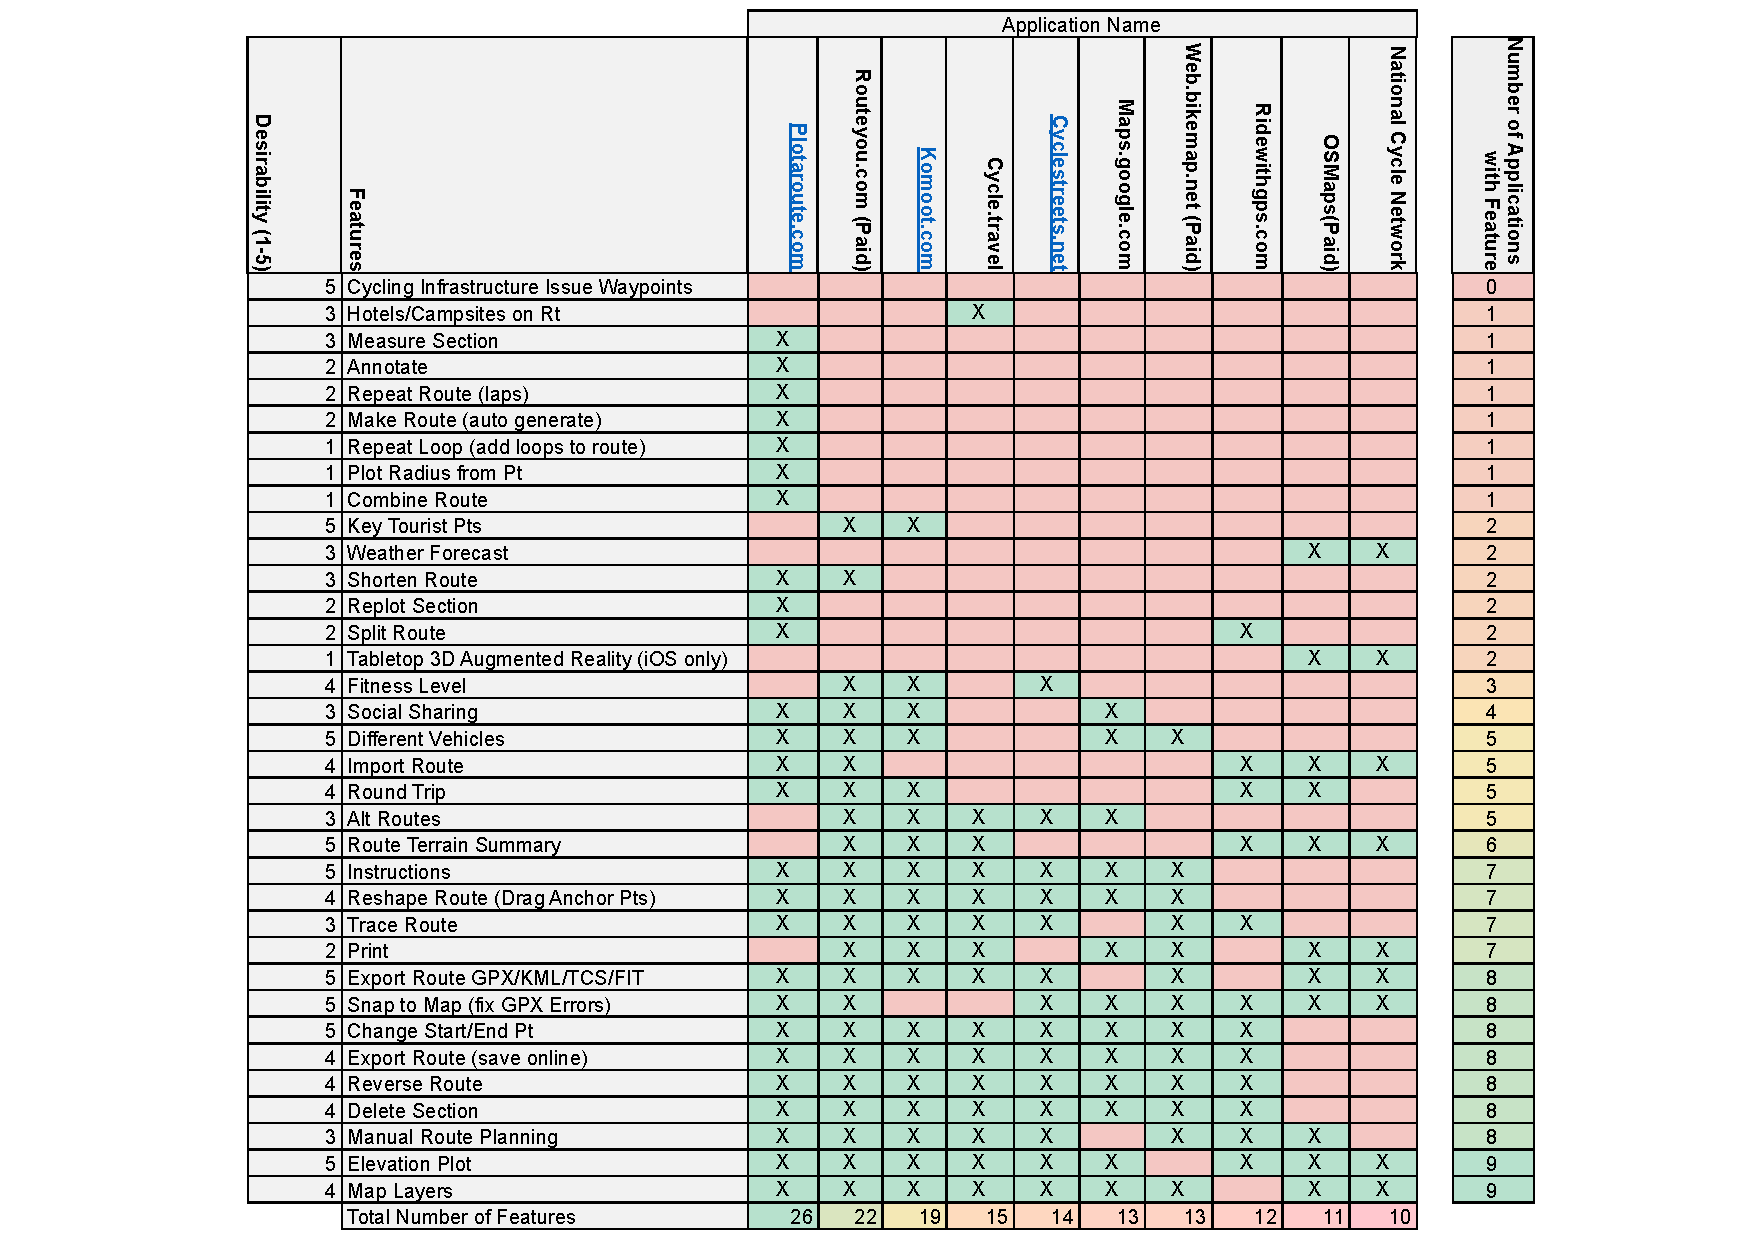
\includegraphics[width=1\linewidth]{figures/current_apps.pdf}
    \caption{Table of current solutions and their included features}
    \label{fig:solutionsandfeatures}
\end{figure}

\subsection{Plotaroute.com}
\label{litrev:plotaroute}
Plotaroute.com (\cite{noauthor_free_nodate}) (Plotaroute), contains a wide range of features, including nearly all features highlighted in Figure 2.1 \see{fig:solutionsandfeatures}. The User Interface (UI) was identified as the primary shortfall of Plotaroute. Its UI is cluttered due to the large number of features present in the application \see{fig:plotarouteui}. For first-time users, it can be initially confusing what each part of the application does. Due to this, at first glace, it's unclear what type of route planner Plotaroute is, which will fundamentally affect a user's initial decision on whether or not to use the application.

\subsection{Komoot}
\label{litrev:komoot}
Komoot (\cite{noauthor_komoot_nodate}) offers a simpler-looking, feature-rich application for planning and discovering routes \see{fig:komootui}. The application has a community focus, whereby users don't necessarily need to plan a route, instead they can discover routes or share their routes. Consequently, this results in the user needing minimal effort when planning shorter, location-specific rides, however Komoot doesn't offer discovery of longer routes. When compared to Plotaroute, Komoot is more user-friendly without sacrificing core features. One primary setback with Komoot is that some route planning functionality is part of a paid-for service, therefore locking certain users out of some desirable functionality.

\subsection{Google Maps}
\label{litrev:gmaps}

Google Maps (\cite{noauthor_google_nodate}) trades the custom cycling functionality for a simple, multi-functional route planning application \see{fig:gmapsui}. Google Maps is likely the most user-friendly out of all the applications, simply due to its consistency across other Google applications (\cite{noauthor_material_nodate}). This has trade-offs, however, most cycling-specific functionality is not present, therefore the routing algorithm is restricted to its default configuration with little customisability.

\label{fig:research-results}
\begin{figure}[h!]
    \centering
    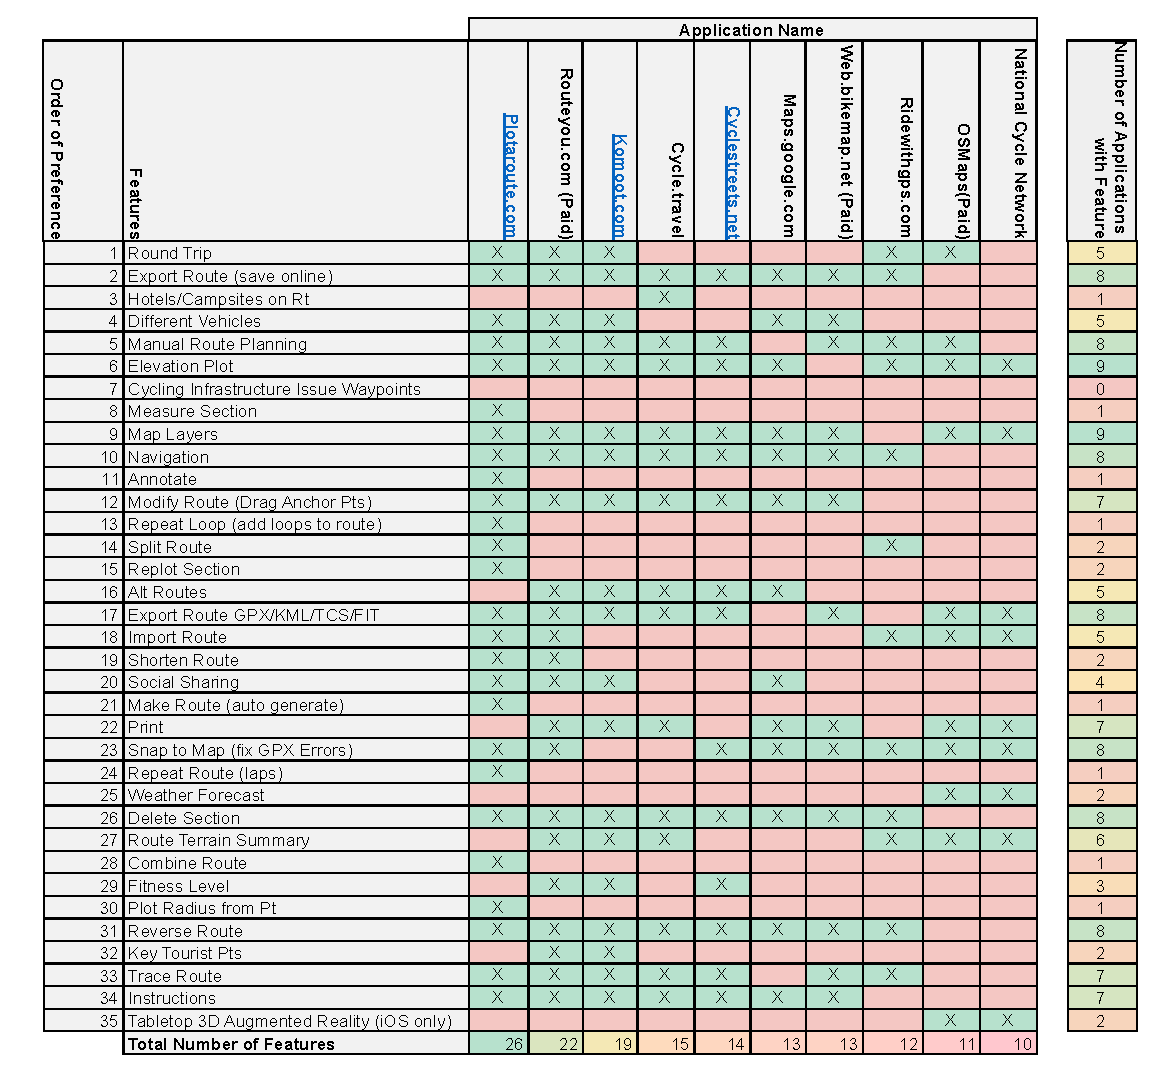
\includegraphics[width=1\linewidth]{figures/current_apps_post_research.pdf}
    \caption{Features in priority order based on user feedback}
    \label{fig:features}
\end{figure}

\section{Risk Factors in Route Planning}
Risk-based cycling route planning requires extensive knowledge of the impact of cycling and transportation infrastructure currently in place. It is also critical to understand how other external factors impact the risk of a route on an ever-changing basis. Within this section, a range of risk factors were explored to understand how multiple risk factors can be implemented into route planning algorithms.

\subsection{Cycling Infrastructure}
\label{litrev:cyclinginfrastructure}
The cycling infrastructure along a route must be understood because it is common for cyclists to share the same infrastructure as motorised vehicles. However, a cyclist has no physical protection if a crash occurs (\cite{reynolds_impact_2009}). There is often purpose-built infrastructure for cyclists, whether bike lanes alongside shared roads or off-road bike paths and this segregated infrastructure can help improve the safety of a route for a cyclist. Furthermore, Hong states how investing in effective cycling infrastructure "mitigates the negative effects of poor weather conditions" (\cite{hong_can_2020}), which further demonstrates that good, known infrastructure is key to improving the physical and perceived safety of a route in a range of different weather conditions. 

Furthermore, crowd-sourced data from route planners, cyclists and fitness applications such as Strava Routes (\cite{noauthor_strava_nodate}) have been key in developing new infrastructure. Boettge states how the most accurate assessment of a cycle network would come directly from the cyclists who use the network (\cite{boettge_assessing_2017}). Cyclists who use the network are the most familiar with the quality of each route and how traffic conditions improve the safety of the route. Utilising the GPS information from route planners and fitness tracking applications alongside direct input from cyclists can help build new routes and improve pre-existing routes, therefore preventing injuries and high-risk situations by modifying transportation infrastructure (\cite{reynolds_impact_2009}).

Areas with little to no cycling infrastructure, such as busy roads and roundabouts, force cyclists to have a heightened attentiveness that other road users don't have to consider due to not only the physical danger but the cyclists' perceived danger (\cite{doorley_analysis_2015}). These risks should be considered within route planning to decrease the number of 'risk' areas along a cyclist's route whilst also giving local areas the incentive to make infrastructure modifications to decrease the number of 'high-risk' points. Therefore, in the long-term, it will mitigate the need for constant action by cyclists to ensure their safety, which will, in turn, influence individuals' decisions to cycle (\cite{reynolds_impact_2009}).

Hull and O'Holleran also demonstrate how cities with a high reputation among cyclists also have safer roads and more attractive infrastructure. The Netherlands scored relatively equally amongst all categories, in comparison to cities with less of a reputation and, therefore, a lower standard of cycling infrastructure \see{fig:bicycleinfrastructurescorestable} \see{fig:bicycleinfrastructurescores} (\cite{hull_bicycle_2014}). This supports how Reynolds et al. further illustrate how investing in cycling infrastructure will greatly incentivise individuals to cycle due to the decreased risk. 

\begin{figure}
    \centering
    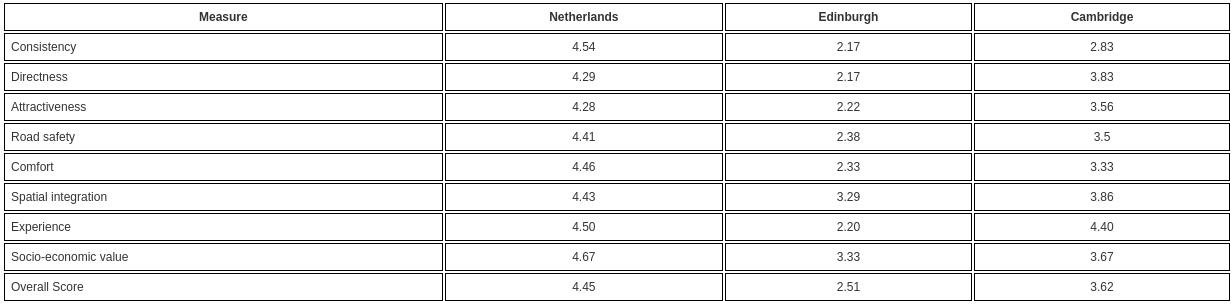
\includegraphics[width=400px, keepaspectratio]{figures/bicycle_infrastructure_score_table.jpg}
    \caption{Comparison of the bicycle infrastructure scores (\cite{hull_bicycle_2014}).}
    \label{fig:bicycleinfrastructurescorestable}
\end{figure}

\begin{figure}
    \centering
    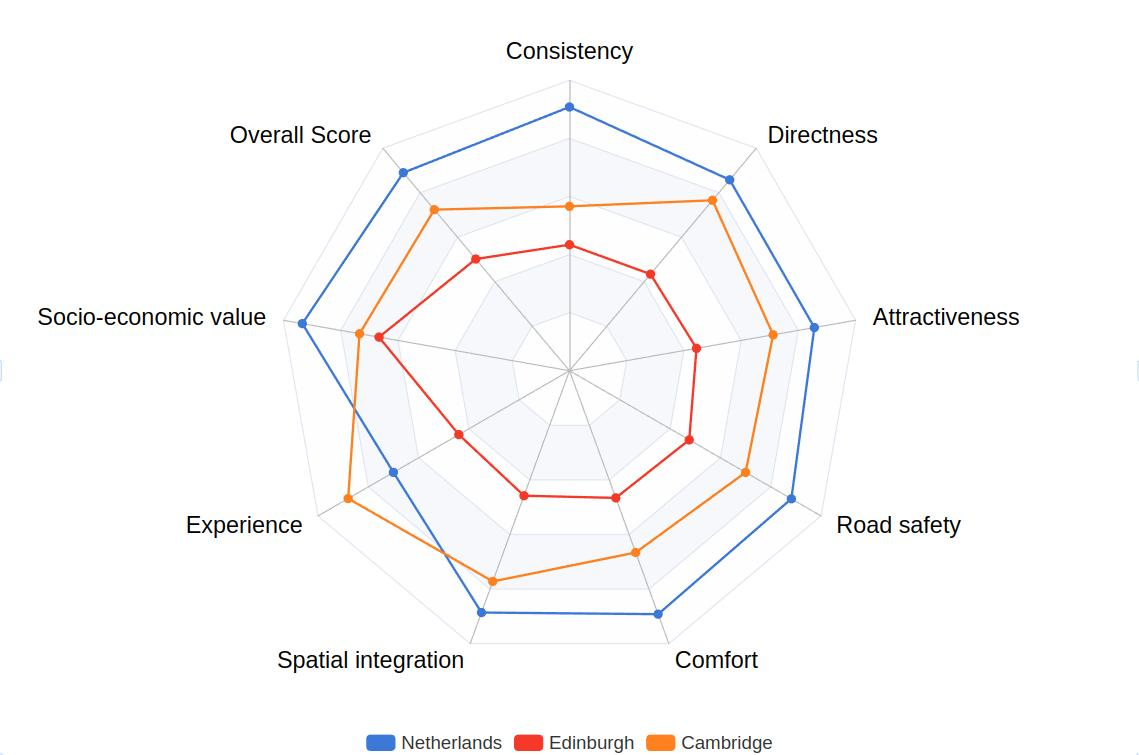
\includegraphics{figures/bicycle_infrastructure_scores.jpg}
    \caption{Spider web diagram comparing the Bicycle Infrastructure Scores (\cite{hull_bicycle_2014}).}
    \label{fig:bicycleinfrastructurescores}
\end{figure}

\subsection{Weather Conditions}
\label{litrev:weatherconditions}
Weather conditions will also have a pivotal effect on how a route planner will calculate the safest route for a cyclist. Following on from Cycling Infrastructure \see{litrev:cyclinginfrastructure}, it is demonstrated how a lack of good infrastructure goes hand-in-hand with creating an unsafe route alongside the weather. To ensure the safety of cyclists, all routes and road surfaces must be maintained to withstand different weather conditions (\cite{shoman_evaluation_2023}).

The weather also impacts a cyclist's likelihood to ride; Flynn states that cyclists `were nearly twice as likely to commute by bicycle when there was no morning precipitation' (\cite{flynn_weather_2012}). Even minor changes in the weather can drastically affect a cyclist's decision to ride, further demonstrating how vital the perceived safety of cycling is in deciding whether to ride. 

Contrasting this, Hull and O'Holleran state that the main environmental barriers included too much traffic, too many hills, no bike lanes/trails, no safe place to cycle and badly maintained streets (\cite{hull_bicycle_2014}). Therefore suggests that the weather should have a minimal impact on a cyclist's decision to ride if the infrastructure is sufficient. Despite the findings of Hull and O'Holleran, it seems to be a common finding that the perceived safety of cycling, both concerning the changing weather conditions and cycling infrastructure, is the primary factor in choosing cycling over an alternative method of transport. Miranda-Moreno and Nosal have shown how when infrastructure is implemented, there is generally an increase in total bicycle usage and diversion of cyclist flows away from roads to purpose-built infrastructure even in less ideal weather conditions (\cite{miranda-moreno_weather_2011}).

\section{Conclusion}
\label{litrev:conclusion}

To conclude, route planning with different customisable preferences has been implemented by a range of different existing organisations; however, focusing on a risk-based routing approach has not been addressed by these existing solutions. Utilising pre-existing routing algorithms such as OpenRouteService (\cite{noauthor_openrouteservice_nodate}) or Open Source Routing Machine (\cite{noauthor_project_nodate}) and integrating custom, weather and infrastructure data alongside the usual user-preferences has not been implemented within existing solutions. Therefore, this enables a unique system to be developed whereby crowd-sourced infrastructure data alongside weather data provided by OpenWeatherMap combined form a risk index utilised in a customised routing algorithm.

\chapter{Methodology}
\label{chap:methodology}

Choosing which Software Development Life Cycle (SDLC) methodology is a key decision at the beginning of any software development project; the methodology demonstrates the expected route that development will take during the project's lifetime. I have decided to use the Iterative methodology whilst integrating key Project Management methods in other team-focused methodologies, such as Agile \see{chap:pm}.

\section{An Iterative Development Methodology}
\label{methodology:chosen}

I have chosen the Iterative Development Model for this project since the Waterfall Model cannot precisely and completely describe the real software development life cycle (\cite{dapeng_liu_case_2011}).
Each iteration will represent a full software life cycle vaguely following the waterfall methodology's structure: Requirements analysis, Design, Development, Testing, and Release. Iterative development allows for more flexibility during the software development process. It is feasible for a solo-development project as it does not require collaboration with other team members as the Agile methodology does.

The Iterative model breaks larger tasks into smaller, more achievable sub-tasks/iterations. Each task can be broken down into all or some of the stages mentioned earlier. Therefore, if some stages are unnecessary for an iteration, they don't need to be followed. Development of the iterations can be managed using a Kanban board. It can also manage progress in completing this document. To see the added benefits of using Kanban, see Section 4.2.

There are some downsides to using the Iterative model, with one key failure of the model being merging changes between iterations. This downfall of the model introduces a discontinuity of design purpose where the user interface and programming interfaces become discontinuous between iterations (\cite{dapeng_liu_case_2011}). To mitigate this issue, a consistent programming interface be implemented to aid in developing easy-to-read source code throughout the development of iterations.
\chapter{Project Management}
\label{chap:pm}

As stated throughout \see{chap:methodology}, the Iterative SDLC model was chosen for this project. All tasks will be managed with GitHub projects Kanban, Table and Milestones functionality. Furthermore, the project will be managed with Git for version control and regular meetings with the project supervisor were scheduled to monitor progress.

\section{GitHub}

\subsection{Kanban Board and Projects}
\label{pm:kanban}

From the beginning, a GitHub project was created with the code repository to manage all development and writing tasks to be completed. All tasks were initially added to the backlog and allocated a milestone and label to categorise each task.

Milestones were created for each iteration of the prototype and each section of this document. Each task would then be assigned a 'To Do' status when selected for development/writing and would progress throughout the other Kanban Board stages until it was marked as 'Done' and closed. This allowed for the effective management of subtasks on a per-milestone and status basis.

An 'In Review' status was added to the Kanban board for tasks that required guidance from the project supervisor \see{pm:supervisor_meetings}.

\subsection{Version Control}
\label{pm:version_control}

GitHub will host the source code with Git Software Version Management (SVM). Using GitHub and Git enables branches to be created in the repository to manage code changes and link each change to a pull request which enables effective iterative development. Branches allow for branch-level testing and pull requests for automated merges once the increment has been completed. These merges will also throw merge conflicts arise between iterations, ensuring the code base remains accurate, forcing the conflict to be resolved before changes are made. Commits are also highly valuable during development as they allow code changes to be managed and reversed if needed. 

\section{Supervisor Meetings}
\label{pm:supervisor_meetings}

With the project requiring regular client interaction, regular meetings were scheduled with the supervisor to monitor progress. In-person meetings were preferred, however, due to illness, video conferences were used as a backup. Due to being ahead of schedule, after the 13th meeting, the meetings comprised mostly personal tutor sessions as the project was in its final stages, therefore, the meetings post this date were not documented. See the list of meetings below:

\begin{itemize}
    \item \textbf{Meeting 1 - 26th September 2023}
    \begin{itemize}
        \item Discussion of the initial project idea.
        \item Discussion of different approaches to the project.
        \item Discussion of the best way to work with the supervisor.
    \end{itemize}
    \item \textbf{Meeting 2 - 5th October 2023}
    \begin{itemize}
        \item Feedback on initial draft project initiation document.
        \item Outlining overall project objectives.
    \end{itemize}
    \item \textbf{Meeting 3 - 11th October 2023}
    \begin{itemize}
        \item Finalise and submit project initiation document.
        \item Discussion of ethics application.
        \item Discussion of potential primary research methods.
    \end{itemize}
    \item \textbf{Meeting 4 - 18th October 2023}
    \begin{itemize}
        \item Demo and feedback of initial research prototype application.
        \item Demo and feedback of initial basic artefact setup.
        \item Discussion of potential future features.
    \end{itemize}
    \item \textbf{Meeting 5 - 25th October 2023}
    \begin{itemize}
        \item Feedback on document progress so far, working towards literature review.
        \item Discussion on ways to rank and compare feedback from the research application.
    \end{itemize}
    \item \textbf{Meeting 6 - 30th October 2023}
    \begin{itemize}
        \item Feedback on literature review.
        \item Discussion of requirements using research feedback.
    \end{itemize}
    \item \textbf{Meeting 7 - 14th November 2023}
    \begin{itemize}
        \item Feedback on complete literature review.
        \item Feedback and discussion of requirements.
        \item Further discussion of potential future features on top of requirements.
    \end{itemize}
    \item \textbf{Meeting 8 - 29th November 2023}
    \begin{itemize}
        \item Requirements mostly finalised, feedback received.
        \item Discussion on the design of the artefact.
    \end{itemize}
    \item \textbf{Meeting 9 - 8th December 2023}
    \begin{itemize}
        \item Final feedback on project so far for 2023.
        \item Discussion of development/sprint plan for January 2024.
        \item Discussion of plan post-development.
    \end{itemize}
    \item \textbf{Meeting 10 - 10th January 2024}
    \begin{itemize}
        \item Feedback on development progress so far.
        \item Agreement made to delay meetings for 3-4 weeks to allow for development.
        \item Agreement on the plan for post-development (3-4 weeks).
    \end{itemize}
    \item \textbf{Meeting 11 - 9th February 2024}
    \begin{itemize}
        \item Feedback on development
        \item Discussion of end-goal, final artefact/document.
        \item Discussion of the plan for the project stages.
    \end{itemize}
    \item \textbf{Meeting 12 - 16th February 2024}
    \begin{itemize}
        \item Feedback on Design and Implementation chapters.
        \item Agreement on final end goal - 5 weeks from 16th February.
        \item Agreement to complete draft of final document within 2 weeks.
        \item Agreement to use final 3 weeks to review and improve.
        \item Discussion of the use of unplanned extra time (after 5 weeks) to improve artefact.
    \end{itemize}
    \item \textbf{Meeting 13 - 23rd February 2024}
    \begin{itemize}
        \item Final guidance provided for last improvements to report.
        \item Discussion on how to use extra time post-easter.
    \end{itemize}
\end{itemize}
\chapter{Requirements}
\label{chap:requirements}

The identification of requirements was critical to the success of the project. Primary research was undertaken to gather an understanding of real user preferences from a list of proposed functionalities as to understand their wants and needs of the application. It was critical to declare clear and concise requirements to ensure absolute clarity thooughout the project. This chapter discusses all methods undertaken to gather requirements, including the final requirements found as a result of this process.

\section{Requirements Gathering}
\label{requirements:gathering}

Requirements were gathered via multiple channels, initially research was undertaken to understand the offerings of current solutions to gather a list of potential functionalities. These were then taken to the client to set out a base set of user requirements to be used in primary research. A simple research application was developed to collect the opinions of cyclists in the general public, enabling participants to order a subset of a wider list in order of preference \see{fig:researchapp}.

\section{Identifying Users}
\label{requirements:identifyingusers}

The aims highlighted the need to expand the route planning functionalities available to cyclists \see{intro:aimsandobjectives}. Multiple user groups were identified from this:
\begin{itemize}
  \item Commuter - A commuter would require a simple round trip route, likely focused on ease of ride and speed taken to commute.
  \item Regular Cyclists - A cyclist who focuses on planning a ride tailored for their skill level. Wants multiple route options with varying levels of intensity.
  \item Pro Cyclists - A pro cyclist would require a deeper level insight into each planned route, including a range of customisability and integration with fitness applications.
\end{itemize}


\section{Requirements Specification}
\label{requirements:specification}

User stories were established through various methods: regular face-to-face meetings were conducted with the client and research was conducted through a web application built to understand the users' preferred functionality \see{fig:researchapp}. Each user story was broken down into specific system requirements. The requirements have been ranked using the MoSCoW model; this demonstrated each requirements' level of importance aiming to prioritise the necessary requirements, limiting the time spent on the less-necessary requirements. The MoSCoW model seemed the most appropriate choice in prioritising requirements because of the research undertaken with real-world users, utilising the data collected on user preferences \see{fig:userfeedback01}\see{fig:features}.

\begin{figure}[!h]
  \centering
  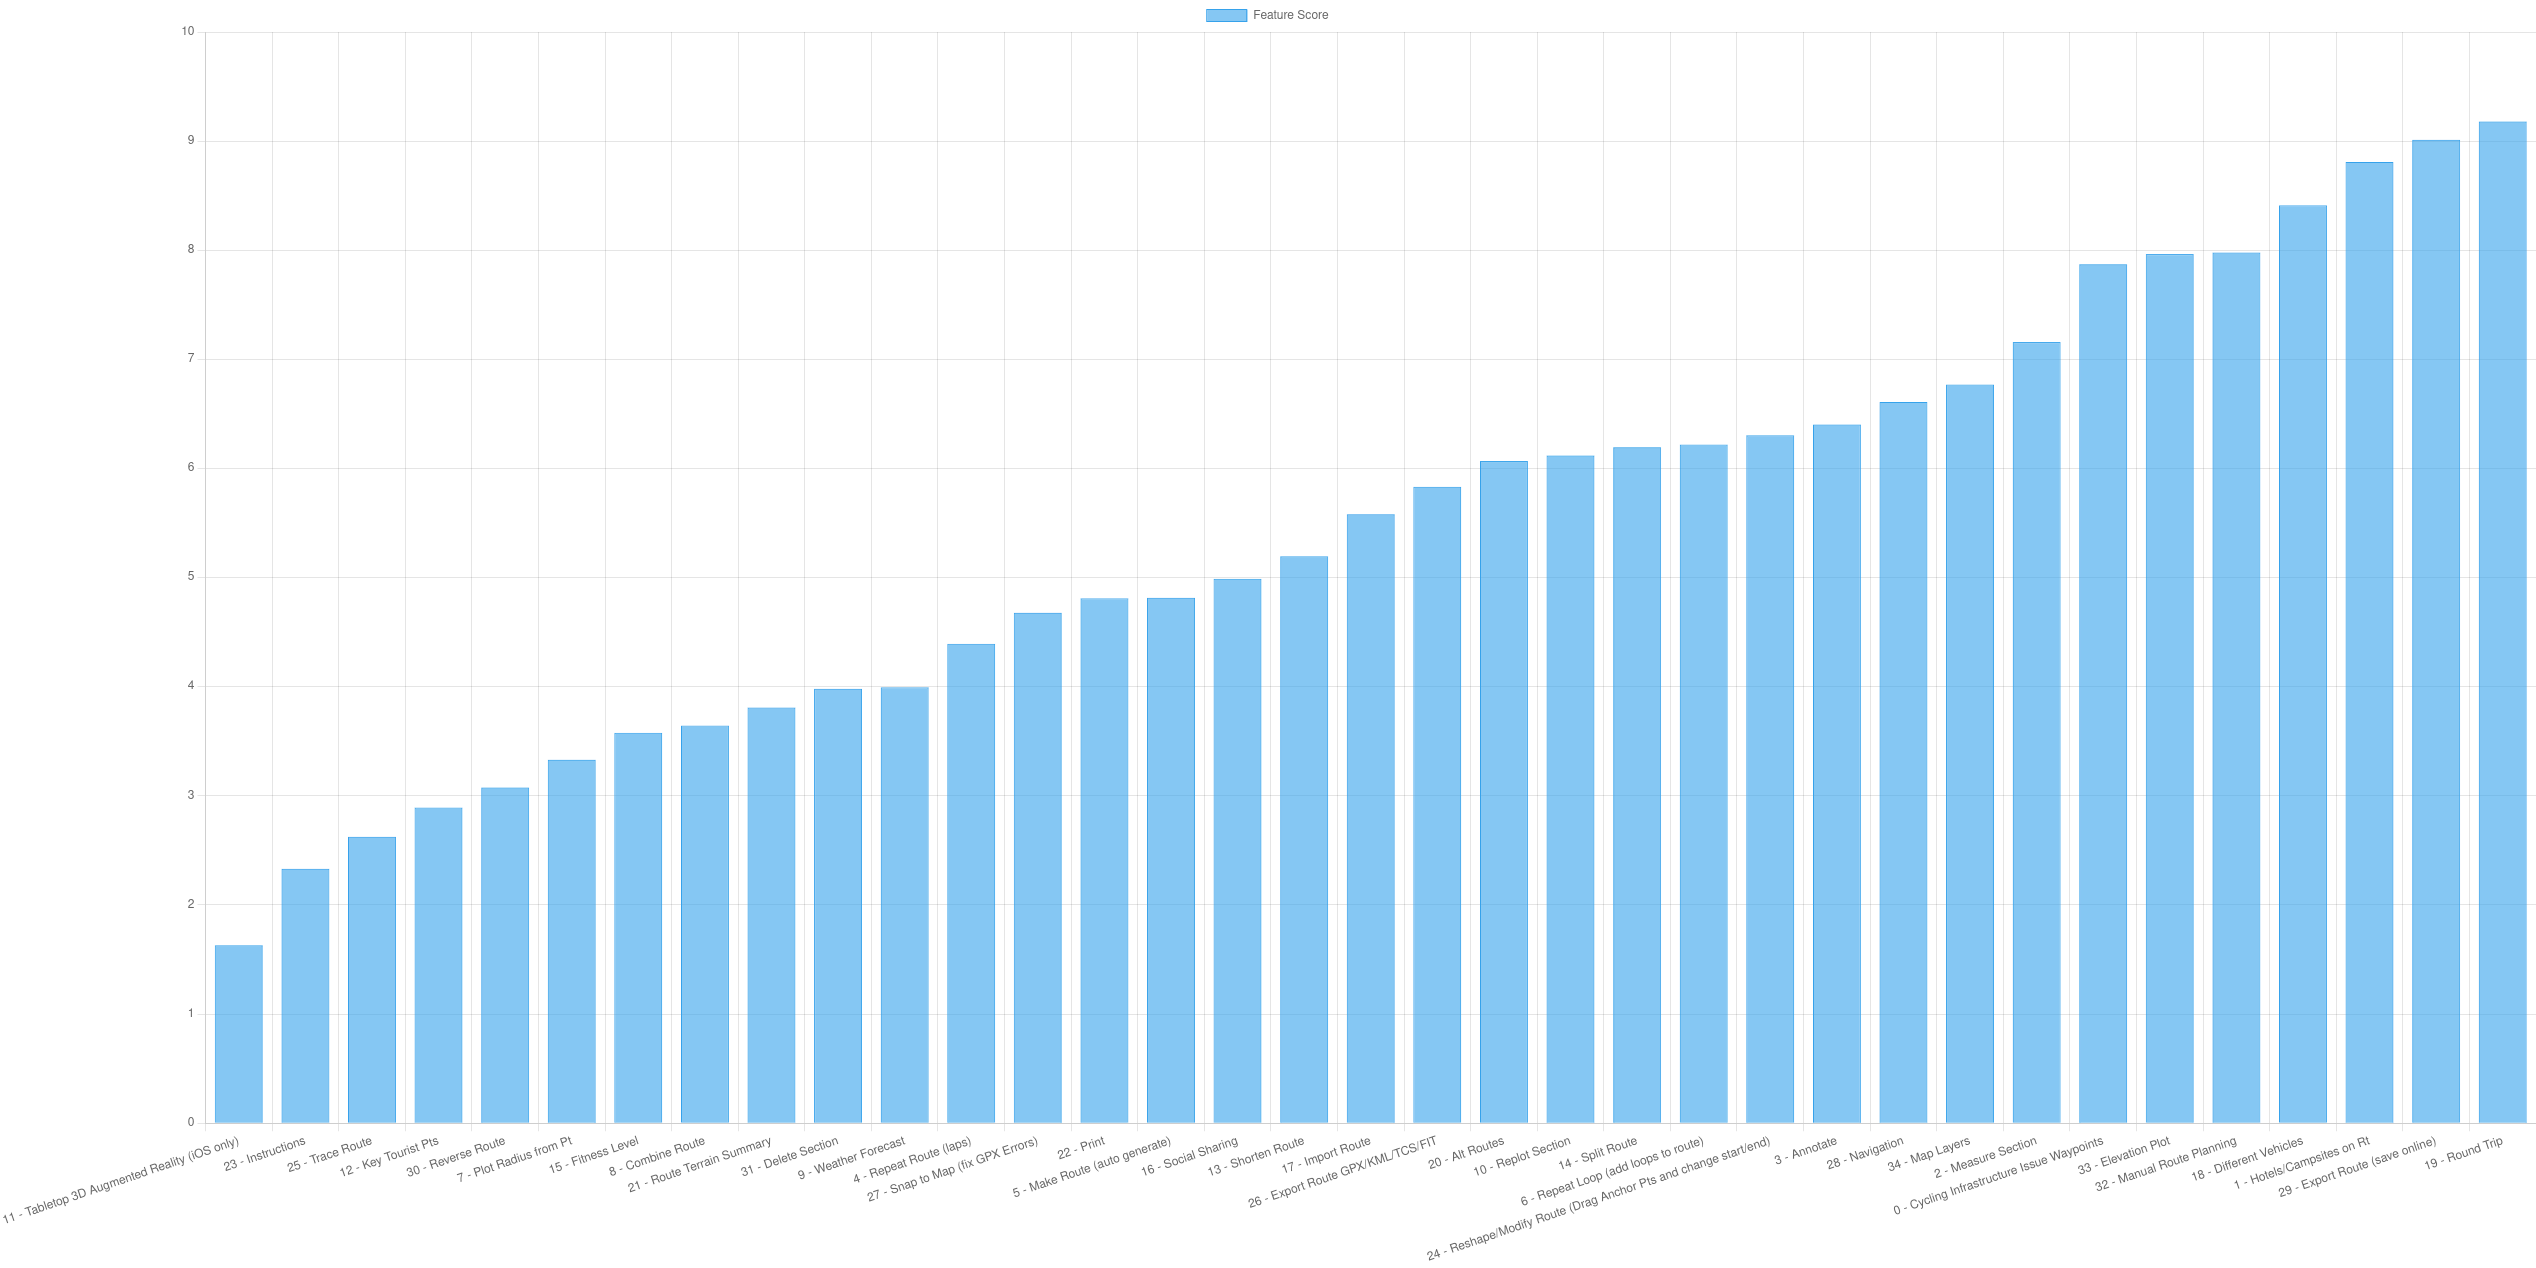
\includegraphics[width=400px]{figures/logarithmic-scoring.png}
  \caption{User Feedback}
  \label{fig:userfeedback01}
\end{figure}

\begin{figure}
  \centering
  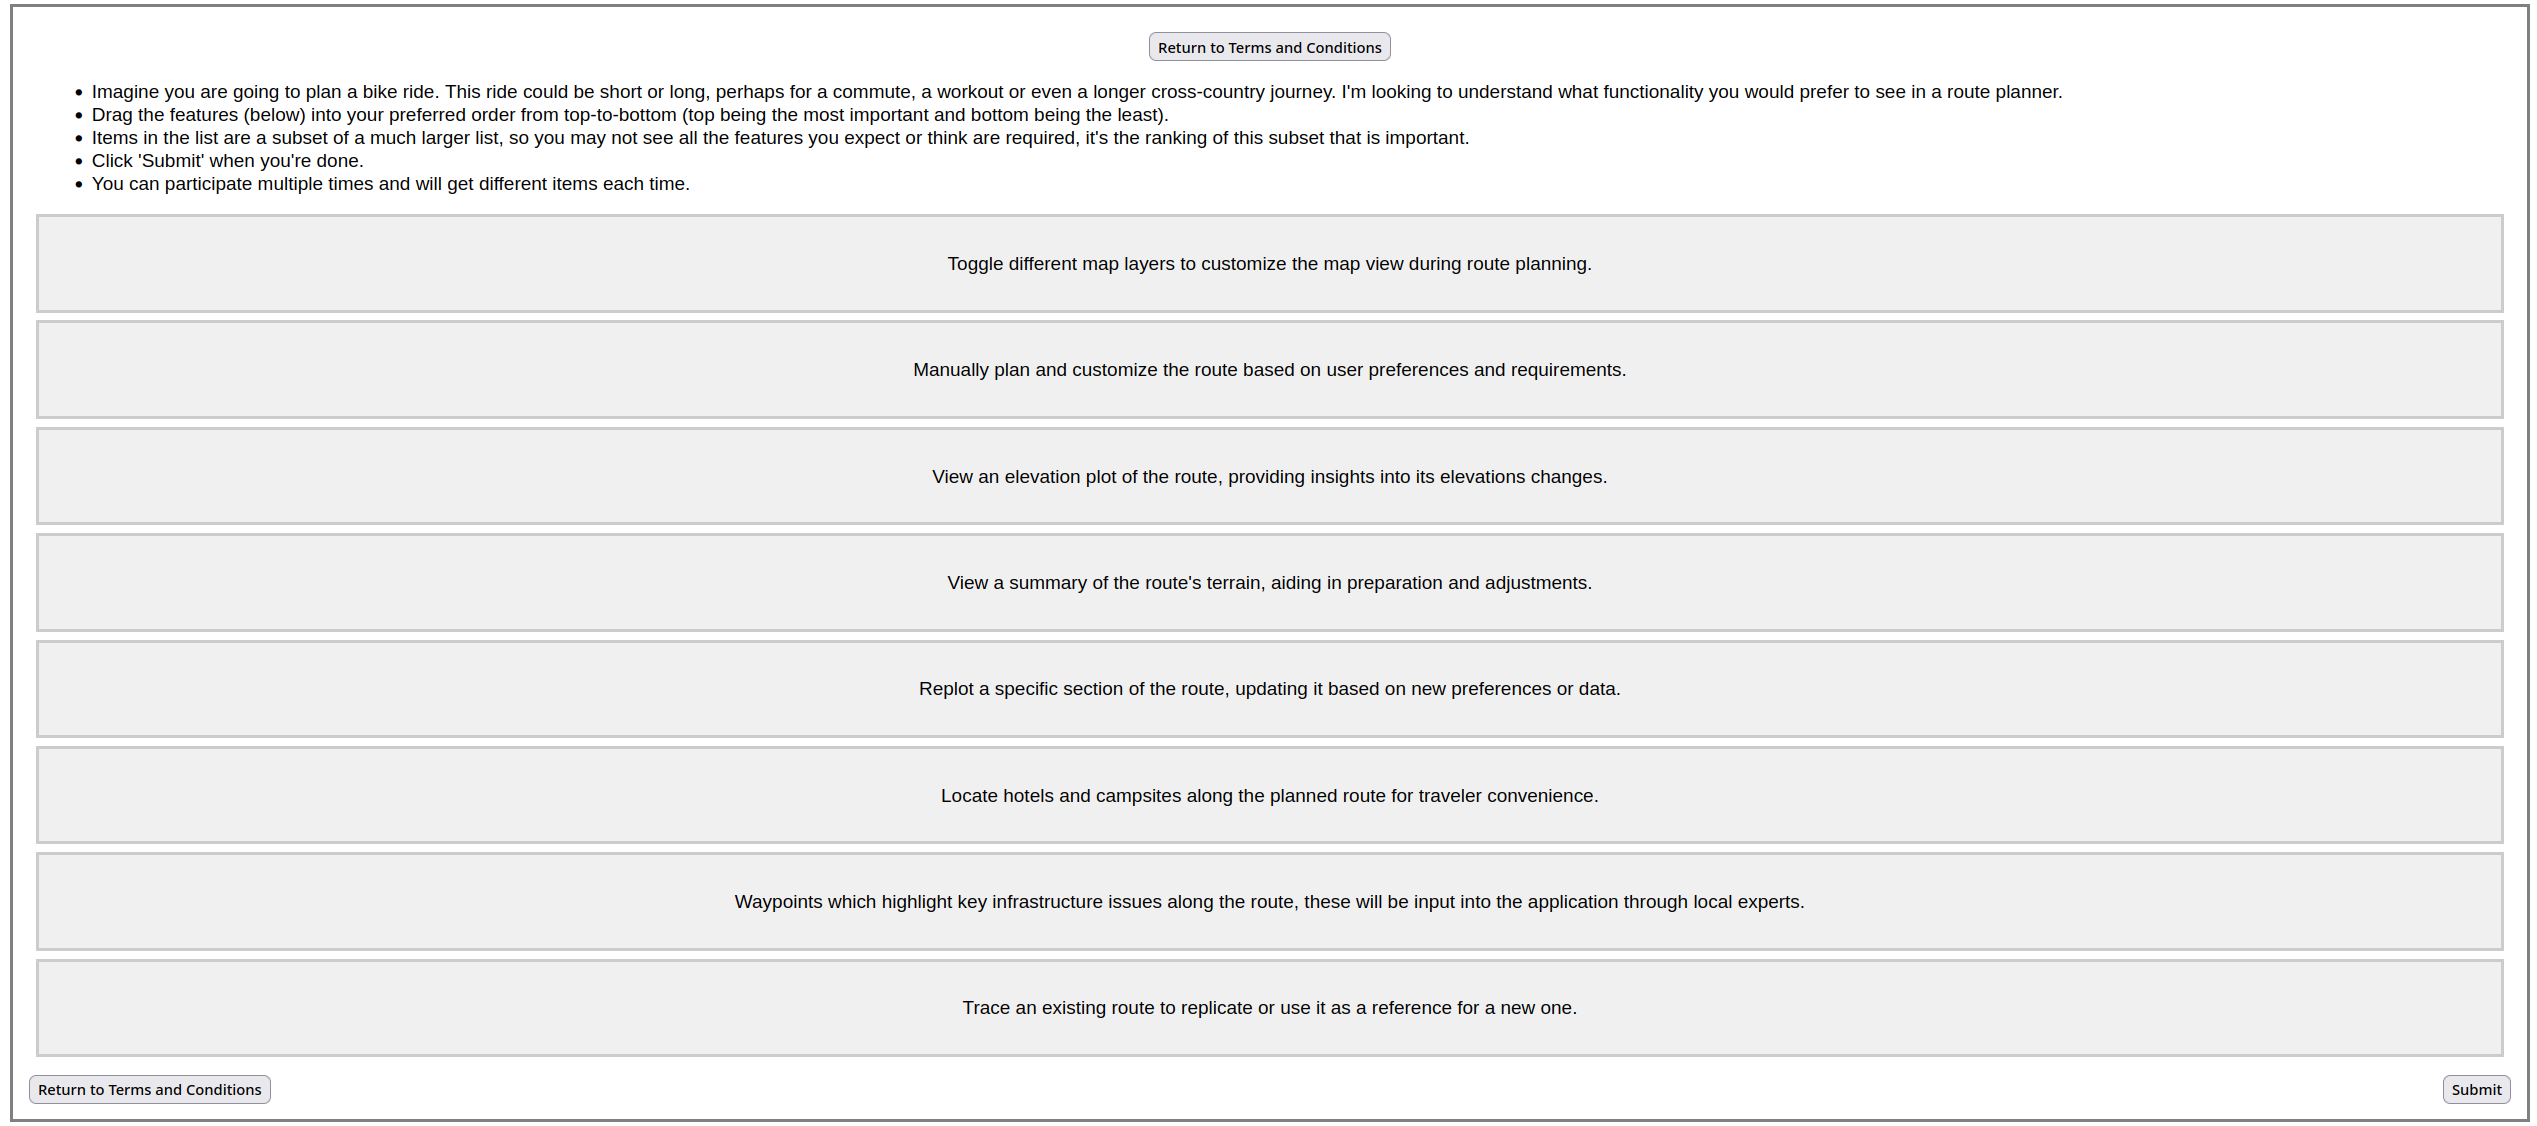
\includegraphics[width=400px]{figures/research-application.png}
  \caption{Firebase Research Application}
  \label{fig:researchapp}
\end{figure}

\clearpage
\section{Elicited Requirements}
\label{requirements:user-stories}

The elicited requirements were a direct result of discussions with the client and the primary research undertaken \see{requirements:specification}. Each user story was divided into multiple acceptance criteria/system requirements and were segregated into a table per user story.

\begin{table}[!htb]
\caption{User Story 01}
\label{tab:user-story-01}
\begin{tabular}{ p{8cm} p{1cm}  p{1cm} }
\hline
\multicolumn{3}{p{13cm}}{As a user, I want a page that allows me to configure my starting and destination location to plan a route.}\\ 
\hline
Acceptance Criteria / System Requirements & Priority & ID\\
\hline
The system must provide a route configuration panel. & Must & SR1\\
The route configuration page must provide a starting and destination location input field. & Must & SR2\\
The route configuration page should suggest accurate geolocations based on the location inputs. & Must & SR3\\ 
The route configuration page must determine the geolocation based on the user input. & Must & SR4\\ 
The route configuration page must plan the route once two or more locations are input. & Must & SR5\\ 
\hline
\end{tabular}
\end{table}

\begin{table}[!htb]
\caption{User Story 02}
\label{tab:user-story-02}
\begin{tabular}{ p{8cm} p{1cm}  p{1cm} }
\hline
\multicolumn{3}{p{13cm}}{As a user, I want to change preferences to allow me to customise the route, including avoiding certain road types and road altitudes.}\\ 
\hline
Acceptance Criteria / System Requirements & Priority & ID\\
\hline
The system must provide an overlay window to allow the user to update routing preferences. & Must & SR6 \\
The update preferences overlay must provide options to 'avoid' along the route. & Must & SR7\\
The update preferences overlay must provide a 'via' user input field. & Should & SR8\\ 
The update preferences overlay must provide a 'leave time' user input field. & Should & SR9\\ 
The update preferences overlay must provide a 'arrive time' user input field. & Should & SR10\\ 
The update preferences overlay must provide a 'round trip' user input field. & Could & SR11\\ 
\hline
\end{tabular}
\end{table}

\begin{table}[!htb]
\caption{User Story 03}
\label{tab:user-story-03}
\begin{tabular}{ p{8cm} p{1cm}  p{1cm} }
\hline
\multicolumn{3}{p{13cm}}{As a user, I want to be able to export the planned route for use on my mobile phone or GPS device.}\\ 
\hline
Acceptance Criteria / System Requirements & Priority & ID\\
\hline
The system must provide an option to export the planned route. & Must & SR12 \\
The system must provide an export feature to export the route to the 'GPX' file format. & Must & SR13\\
The system must provide an export feature to export the route to the 'GeoJSON' file format. & Should & SR14\\ 
The system must provide an export online (to Google Drive, OneDrive and/or other cloud services) & Must & SR15\\
\hline
\end{tabular}
\end{table}

\begin{table}[!htb]
\caption{User Story 04}
\label{tab:user-story-04}
\begin{tabular}{ p{8cm} p{1cm}  p{1cm} }
\hline
\multicolumn{3}{p{13cm}}{As a user, I want to share my route with other people.}\\ 
\hline
Acceptance Criteria / System Requirements & Priority & ID\\
\hline
The system must provide a share functionality overlay. & Should & SR16 \\
The share overlay must provide an option to share direct over email. & Should & SR17\\
The system must provide an option to share the route direct to Strava. & Could & SR18\\ 
\hline
\end{tabular}
\end{table}

\begin{table}[!htb]
\caption{User Story 05}
\label{tab:user-story-05}
\begin{tabular}{ p{8cm} p{1cm}  p{1cm} }
\hline
\multicolumn{3}{p{13cm}}{As a user, I want to be provided with route suggestions based on predicted weather conditions over the week.}\\ 
\hline
Acceptance Criteria / System Requirements & Priority & ID\\
\hline
The system must provide the user with a weather condition overlay. & Must & SR19 \\
The weather condition overlay must provide the user with the weather for the current day. & Must & SR20\\
The weather condition overlay must provide the user with the weather for the next week. & Should & SR21\\
The weather condition overlay must provide the user with the option to enable weather conditions in the route planning algorithm. & Could & SR22\\ 
The weather condition overlay must provide the user with suggestions on the best days to cycle. & Could & SR23\\
An option to include weather in route planning should be provided, ensuring the user enters the planned day to ride & Could & SR24\\ 
\hline
\end{tabular}
\end{table}

\begin{table}[!htb]
\caption{User Story 06}
\label{tab:user-story-06}
\begin{tabular}{ p{8cm} p{1cm}  p{1cm} }
\hline
\multicolumn{3}{p{13cm}}{As a user, I want to view the route in detail and get information about parts of the route.}\\ 
\hline
Acceptance Criteria / System Requirements & Priority & ID\\
\hline
The system must provide the user with an interactive map to display the planned route. & Must & SR24 \\
The interactive map must allow the user to zoom into parts of the planned route. & Must & SR25\\
The interactive map must allow the user to select parts of the route and receive detailed information about that subsection of the route. & Should & SR26\\
The interactive map must allow the user to select and drag the planned route to modify its path. & Should & SR27\\ 
The system must display an elevation graph for the planned route beneath the interactive map. & Should & SR28\\
The system must allow the user to measuer chosen sections of the route & Must & SR28\\
The system must provide multiple map layers to give users the greater options when viewing the route & Must & SR29\\ 
\hline
\end{tabular}
\end{table}

\begin{table}[!htb]
\caption{User Story 07}
\label{tab:user-story-07}
\begin{tabular}{ p{8cm} p{1cm}  p{1cm} }
\hline
\multicolumn{3}{p{13cm}}{As a user, I want the ability to add and utilise hazard/infrastructure waypoints ot be considered in route planning.}\\ 
\hline
Acceptance Criteria / System Requirements & Priority & ID\\
\hline
The system must provide a user input modal to input Hazard and Infrastructure Data. & Must & SR30 \\
The hazard input modal must provide a Type drop-down menu based on the OSM Hazard Types. & Must & SR31\\
The hazard input modal must provide a date entry point to specify the date the hazard was seen. & Should & SR32\\
The hazard input modal must provide a submit button to add the hazard to the hazard index. & Must & SR33\\
The infrastructure input modal must provide a Type drop-down menu with different types of cycling/road infrastructure & Must & SR34\\
The infrastructure input modal must provide a date entry point to specify when the bad infrastructure was found & Must & SR35\\
The infrastructure input modal must provide an input box providing the user with the option to supply more detail & Should & SR36\\
Both Hazard and Infrastructure data should be displayed on the map, with an option to toggle on/off, and report errors & Should & SR37\\
\hline
\end{tabular}
\end{table}

\chapter{Design}
\label{chap:design}

This chapter explains the design process undertaken considering both the research found within the literature review \see{chap:litrev} and the established requirements \see{chap:requirements}.
\section{Assumptions and Decisions Taken}
\label{design:assumptions/decisions}

Discussions with the client required specific assumptions and decisions to be made to assit in the project's overall development and progression.

A decision was made to build the application as a web app, primarily to aid with accessibility and device compatibility of the artefact, this type of application also opens the artefact up to a large pre-existing userbase with greater ease. Different screen sizes have been acommodated for with the use of CSS media queries, however the artefact is aimed at desktop route planning, with the potential to be expanded to support mobile devices in the future. 

It was assumed that the target users would have a preexisting knolwedge of route planning and had used similar systems in the past. Due to this, instructions to use the application were not provided as a part of the artefact. Futhermore, a minimal user interface approach was used when developing the artefact to ensure the apps ease of use, whilst enabling key custom route planning functionality \see{design:ui}.

Research was undertaken into different available open source routing algorithms, finally deciding to implement Open Route Service (\cite{noauthor_openrouteservice_nodate}) due to its customisability and native support of round trip route planning.

Specific data sets were stored within the browser LocalStorage, this was chosen for certain data such as user authentication tokens, last route plotted and other data which needed storing between browser sessions. Data sets such as the previous planned route (and related data sets) enabled the user to load the previous route when opening the application after having closed the tab/browser previously. Other data sets such as user tokens, enabled the application to remain logged into external services such as Strava (\cite{noauthor_strava_nodate}), Garmin Connect (\cite{international_garmin_nodate}) and Google Drive (\cite{noauthor_home_nodate}), only requiring the user to reauthenticate once these tokens had expired.

\section{User Interface}
\label{design:ui}
Initially, multiple hand-drawn low-fidelity protoype was created to demonstrate two iterations of the artefact \see{fig:lofi1}, demonstrating some design changes and new features in the second low-fidelity prototype \see{fig:lofi2}. After the low-fidelity prototypes were complete, a high fidelity prototype was created based on the second design using MarvelApp (\cite{noauthor_marvel_nodate}).

The following 5 components form the overall User Interface (UI): Map,  Elevation Chart, Router, Route Preferences Panel and the Weather/Side Panel. The primary component which most other components were dependant on was the Map component; each other component would add enhanced functionality to the artefact.

\subsection{Colour Scheme}
\label{ui:colourscheme}

The plain and simple colour scheme was chosen for simplicity and ease-of-use of the artefact. Despite dark mode being considered for the artefact, it was chosen against after conducting research on pre-existing route planners, it was found that a light map, and surrounding UI was generally considered more usable to the average user. A dark mode could be implemented in the future, enabling the user to switch modes should they choose, also altering the map layer to the corresponding dark/light theme.

\subsection{Low Fidelity Prototype}
\label{ui:low-fi}

Low-fidelity protoyping was vital in the project's early stages, ensuring that all UI elements would meet the user expectations and requirements. The project's clear focus on enhanced routing features, it was critical to ensure that the initialy designs were kept simple, to maximise usability, whilst still including all the required, key functionality. Two iterations were divided into two separate low-fidelity prototypes, where the first demonstrates the core functionality \see{fig:lofi1}, whereas the second also includes some extra functionality, for example the Hazard Index \see{fig:lofi2}.

\subsection{High-Fidelity Prototype}
\label{ui:hi-fi}

The high-fidelity prototype was made after low-fidelity prototyping has concluded. The second low-fidelity prototype was expanded upon at this stage, keeping the design simple, whilst ensuring the required functionality could be implemented. It was critical to ensure tthe high-fidelity protype wouldn't overbare the user with too much information at once, therefore the necessary functionality is available in the main view \see{fig:hifi1}, whereas extra options are hidden behind dropdown menus \see{fig:hifi2}.

  \begin{figure}[!ht]
    \centering
    \includegraphics[width=350px]{figures/lofi-1.png}
    \caption{Low-Fidelity Prototype 1}
    \label{fig:lofi1}
  \end{figure}

  \begin{figure}[!ht]
    \centering
    \includegraphics[width=350px]{figures/lofi-2.png}
    \caption{Low-Fidelity Prototype 2}
    \label{fig:lofi2}
  \end{figure}

  \begin{figure}[!ht]
    \centering
    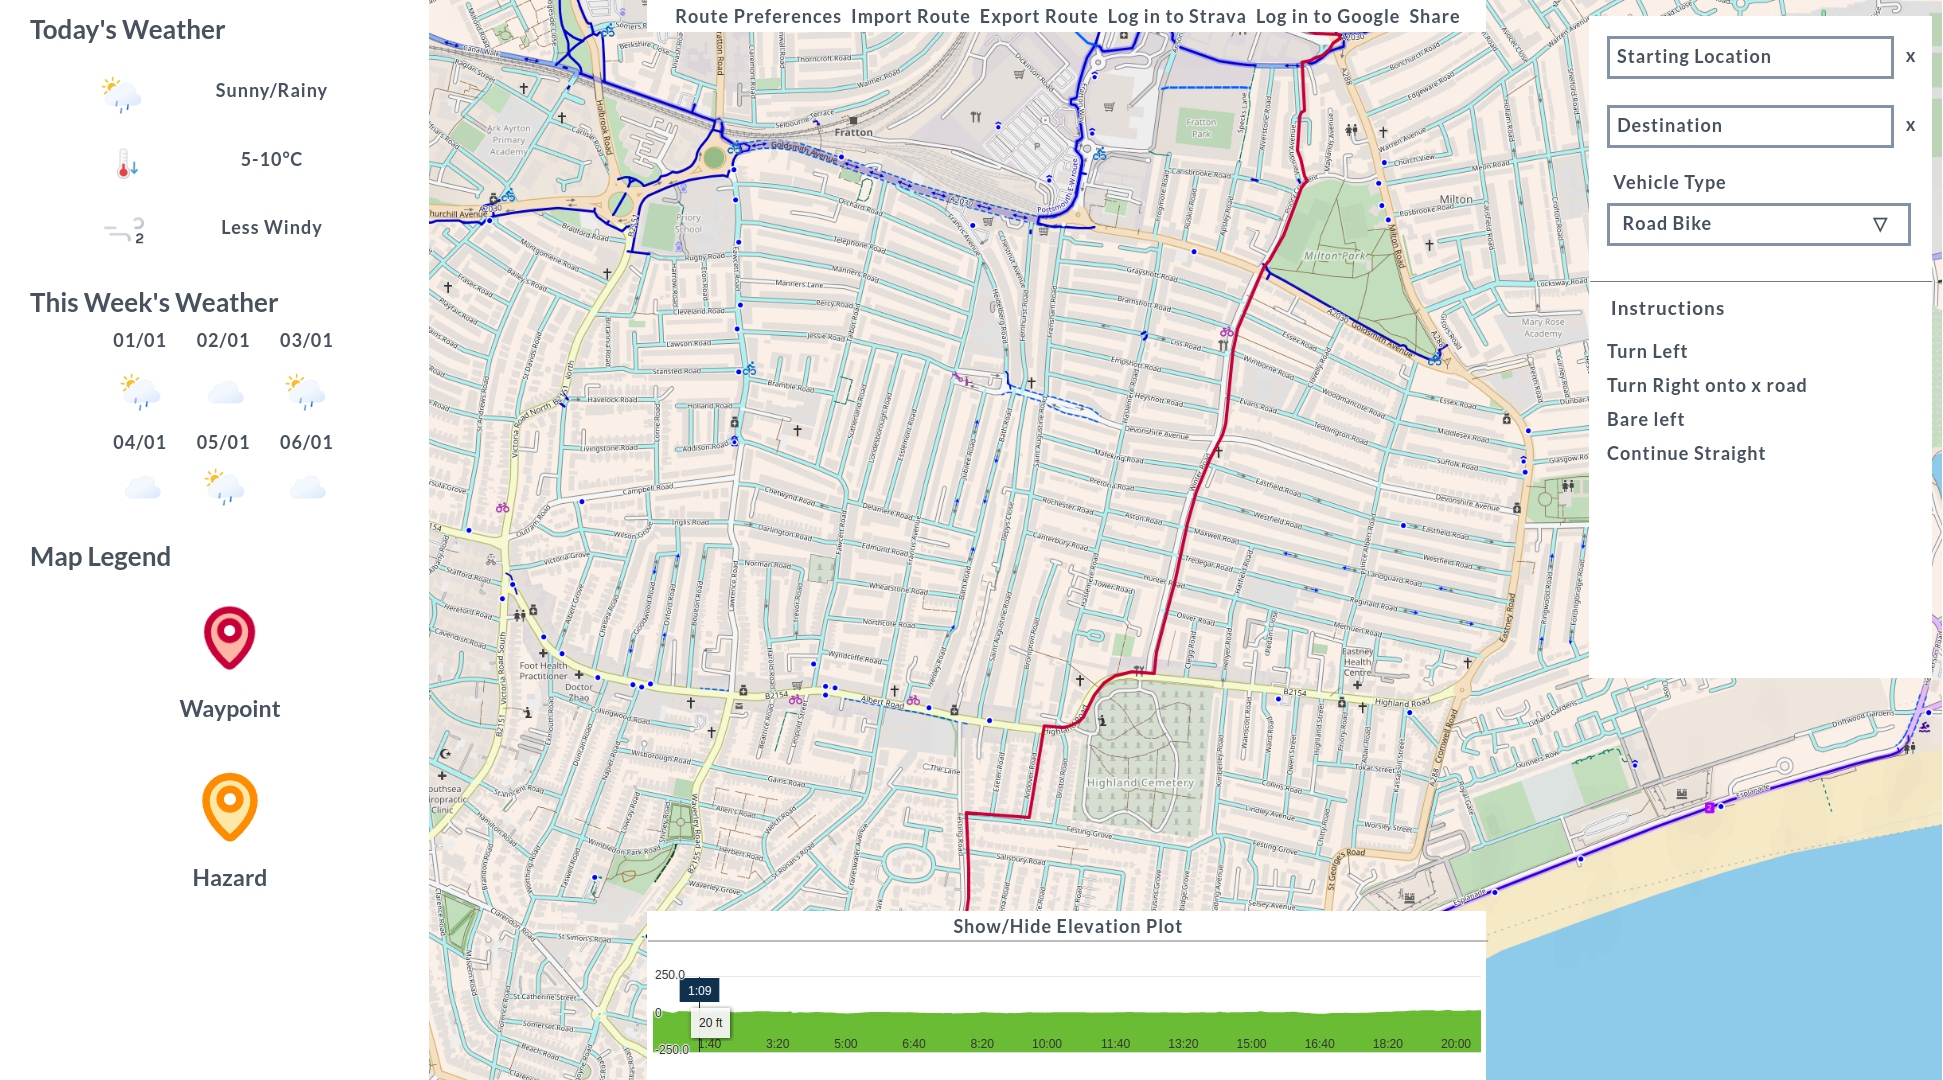
\includegraphics[width=400px]{figures/hifi-1.png}
    \caption{High-Fidelity Prototype 1}
    \label{fig:hifi1}
  \end{figure}

  \begin{figure}[!ht]
    \centering
    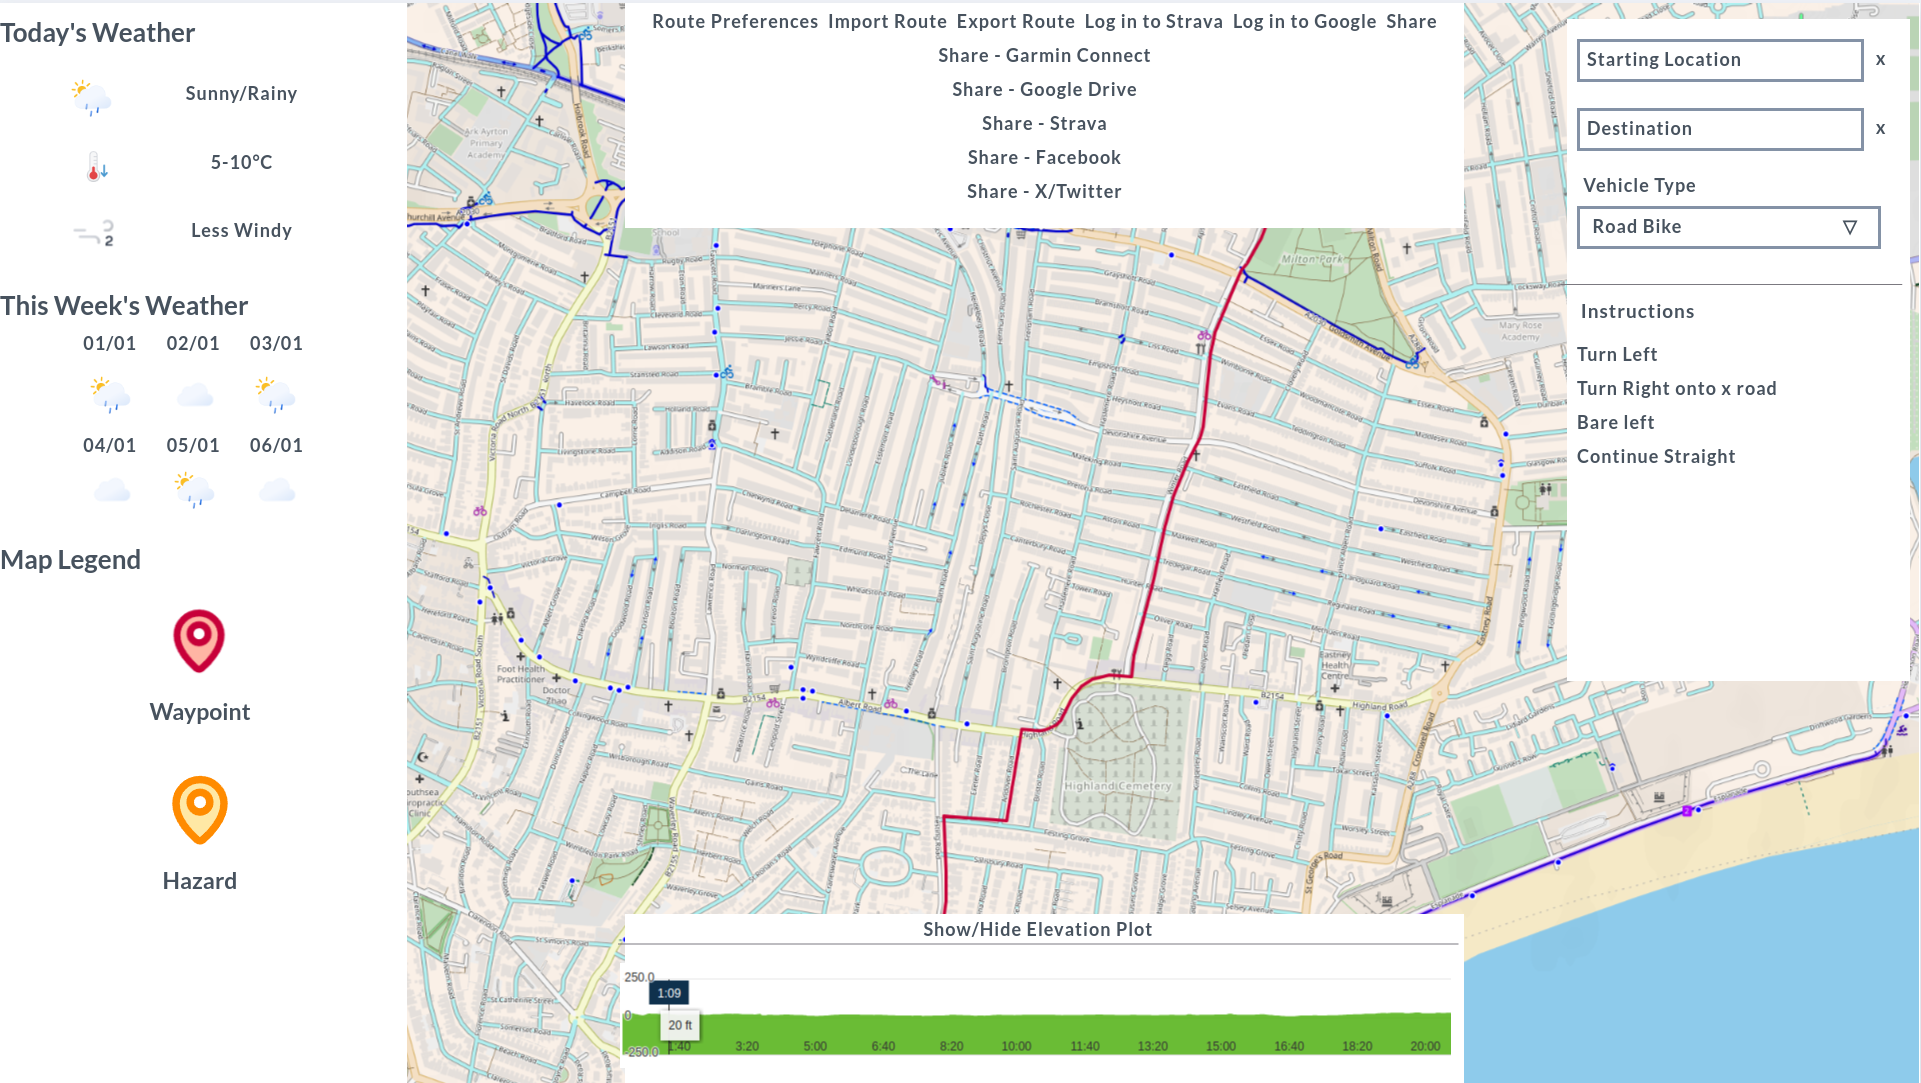
\includegraphics[width=400px]{figures/hifi-2.png}
    \caption{High-Fidelity Prototype 2}
    \label{fig:hifi2}
  \end{figure}

  \clearpage
\section{Use Cases}
\label{design:usecase}
Use cases were determined by discerning potential uses of the artefact, subsequently a use case diagram was then created to visualise the artefacts different uses. The diagram is formed of actors, tasks and system components which are requred to response when each task is performed. Visual Paradigm was used to create the use case diagram (\cite{noauthor_ideal_nodate}).

\subsection{Use Case Diagram}
\label{usecase:diagram}
During the requirements gathering process, the target user groups were identified, each user group would access identical functionality \see{chap:requirements}, therefore all users were grouped into one single actor. Doing so enables all users to access all functionalities of the artefact, where they can use as little or as many of the extended features as they require \see{fig:usecase}.

\begin{figure}[!ht]
  \centering
  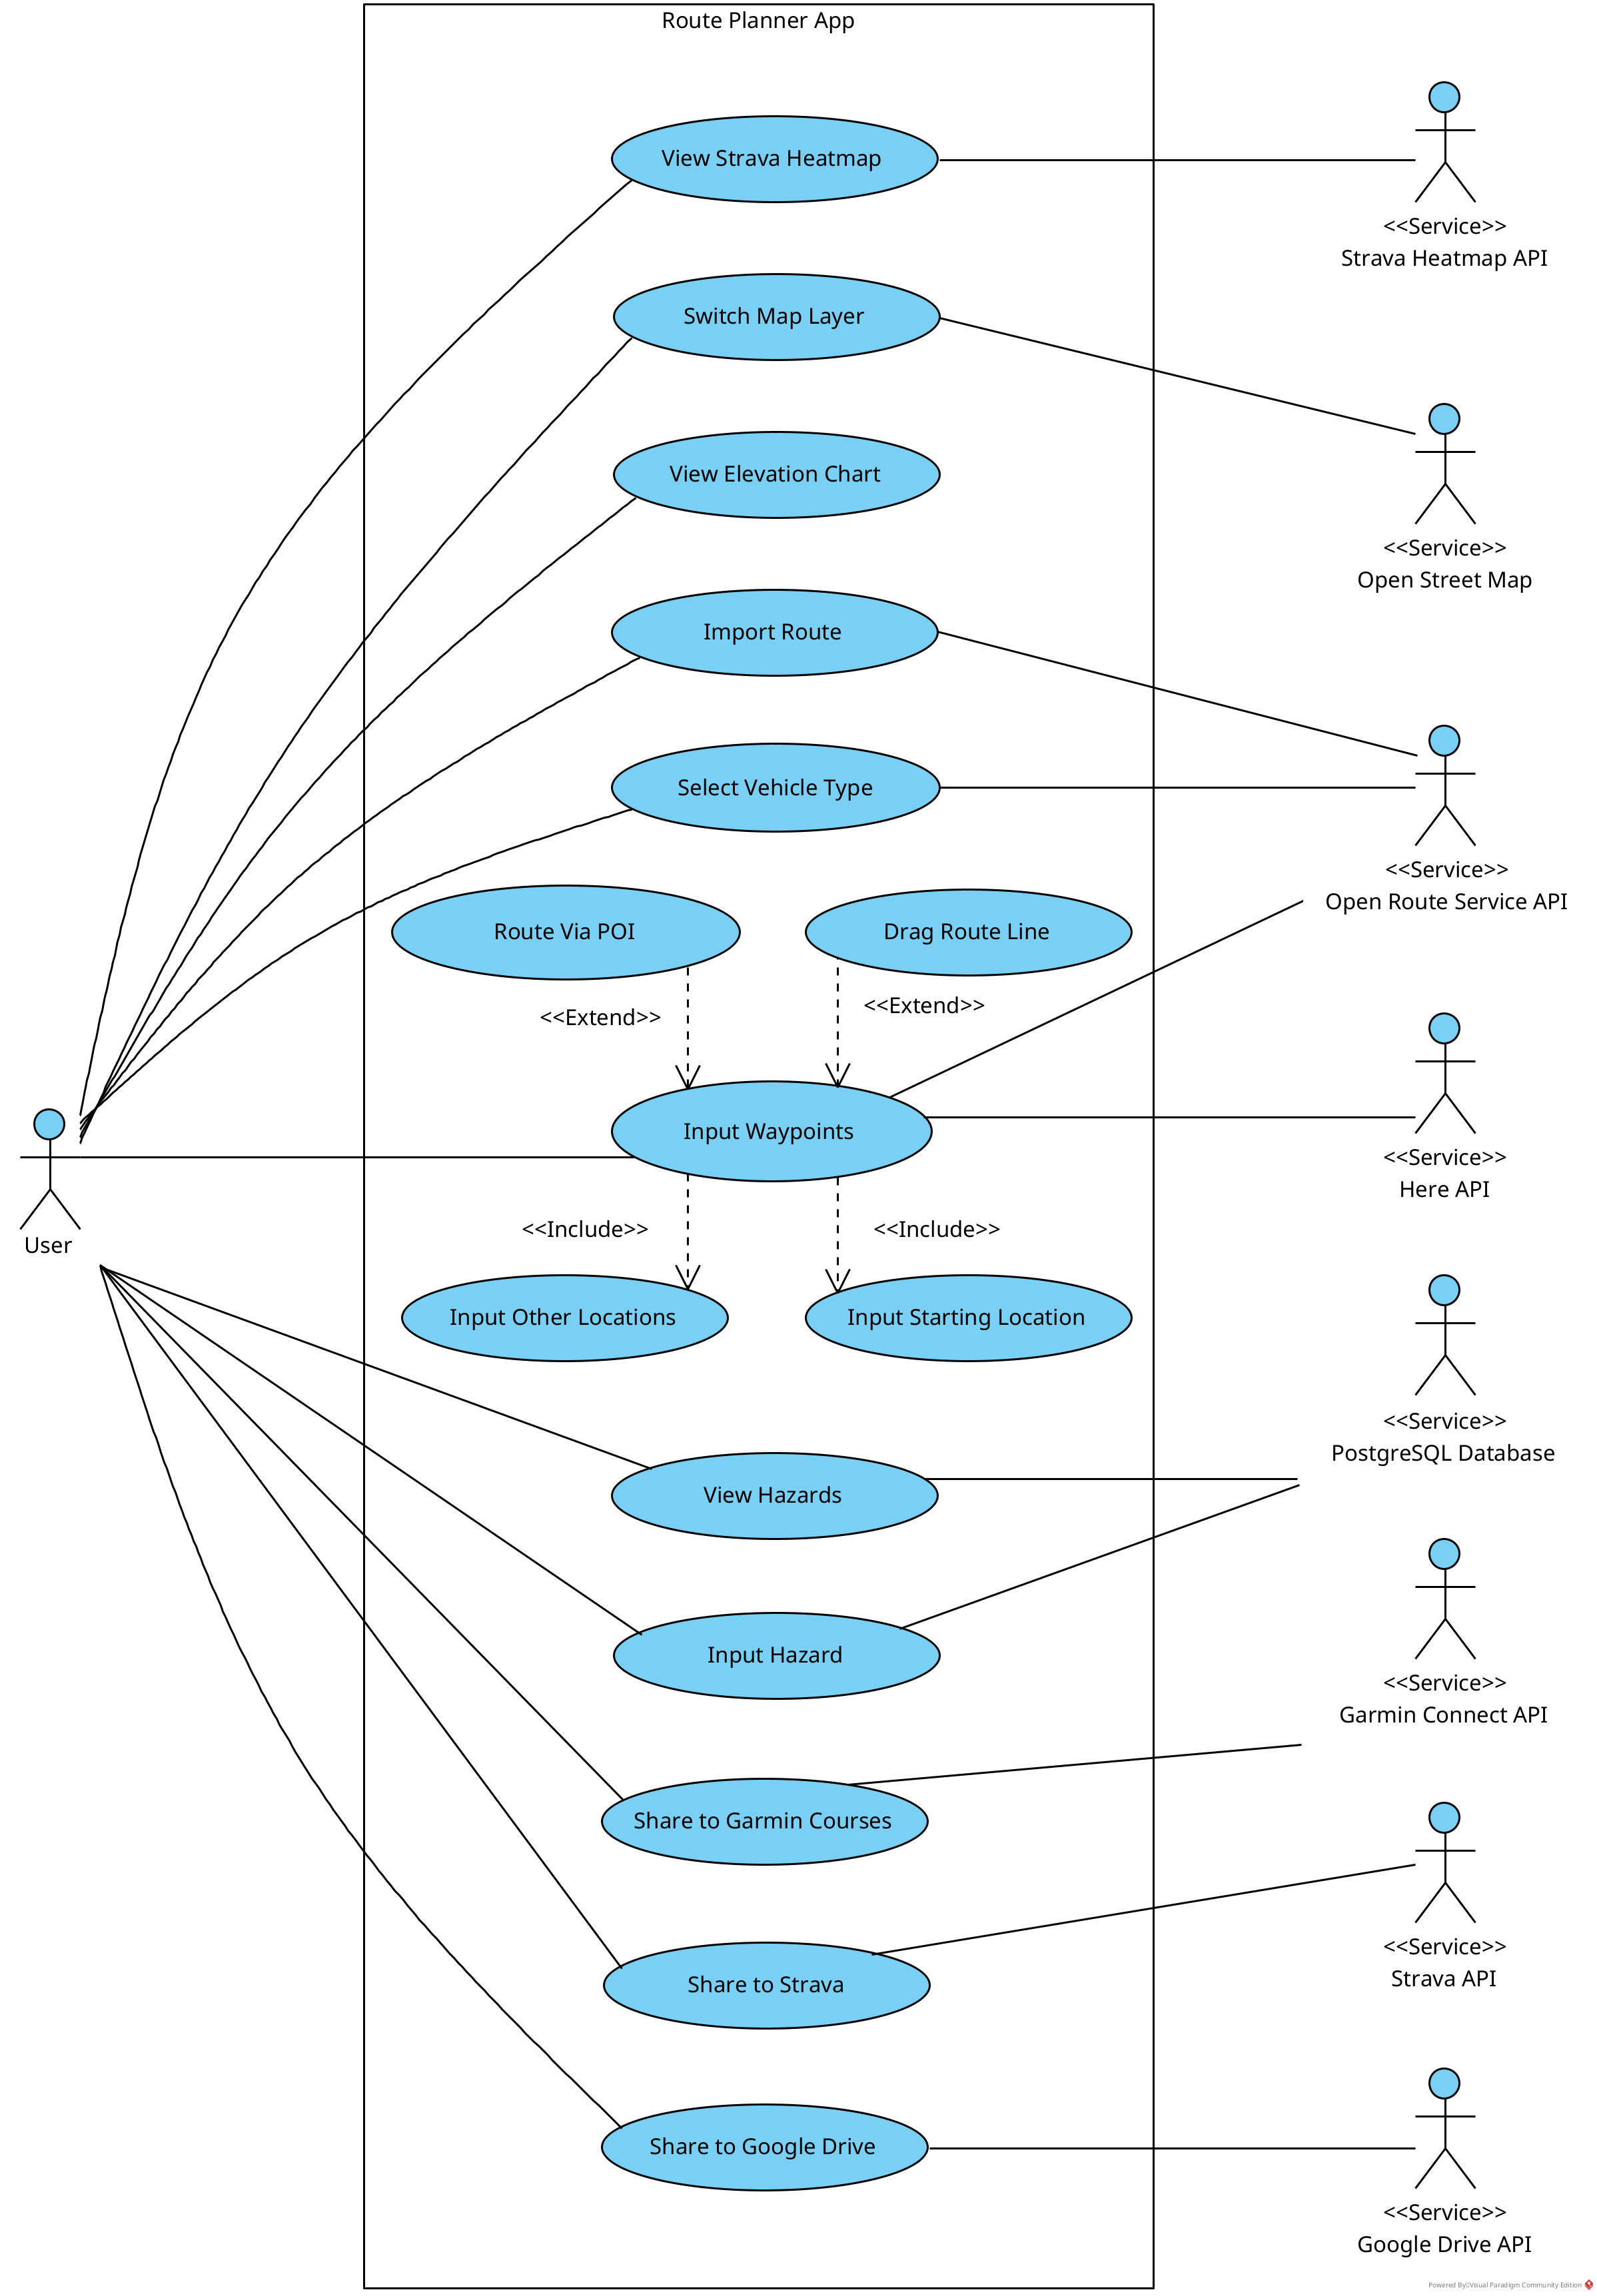
\includegraphics[width=400px]{figures/use-case.png}
  \caption{Use Case Diagram}
  \label{fig:usecase}
\end{figure}

\section{System Design}
\label{design:system}

It is vital to design not only the viewable client-side of the application, but to also consider the internal system, comprising of the Go Gin Web Server, PostgreSQL database as well as the React.js client. This chapter delves further into the internal design of the artefact. 

\subsection{Architecture Design}
\label{system:architecture-design}

The client-server architecture was used to build the artefact \see{fig:clientserver}. This architecture was selected to enable easy expansion of the artefact, with the aim for the web application to be hosted centrally, along with the PostgreSQL (PSQL) database \see{system:database-design}. For security reasons, it was also necessary to implement this architecture due to different services requiring oauth, these services make enforce authentication through the server, rather than completely on the client-side application. Furthermore, this architecture enabled different processes to be handled via the server, reducing the overall load the client application requires to run.

Client-Server architectures do however, add the risk of a single point of failure, whereby the application is wholly dependant on the web server. Overall the risk was deemed minimal due to the lack of sensitive information being stored \see{tab:risk-assessment}. In the case of a system failure, the application would remain unaccessable until fixed, however there is a low chance of this occurring as the appropriate measures such as thorough testing have been undertaken to reduce the risk \see{chap:testing}.

\clearpage
\begin{figure}[!ht]
  \centering
  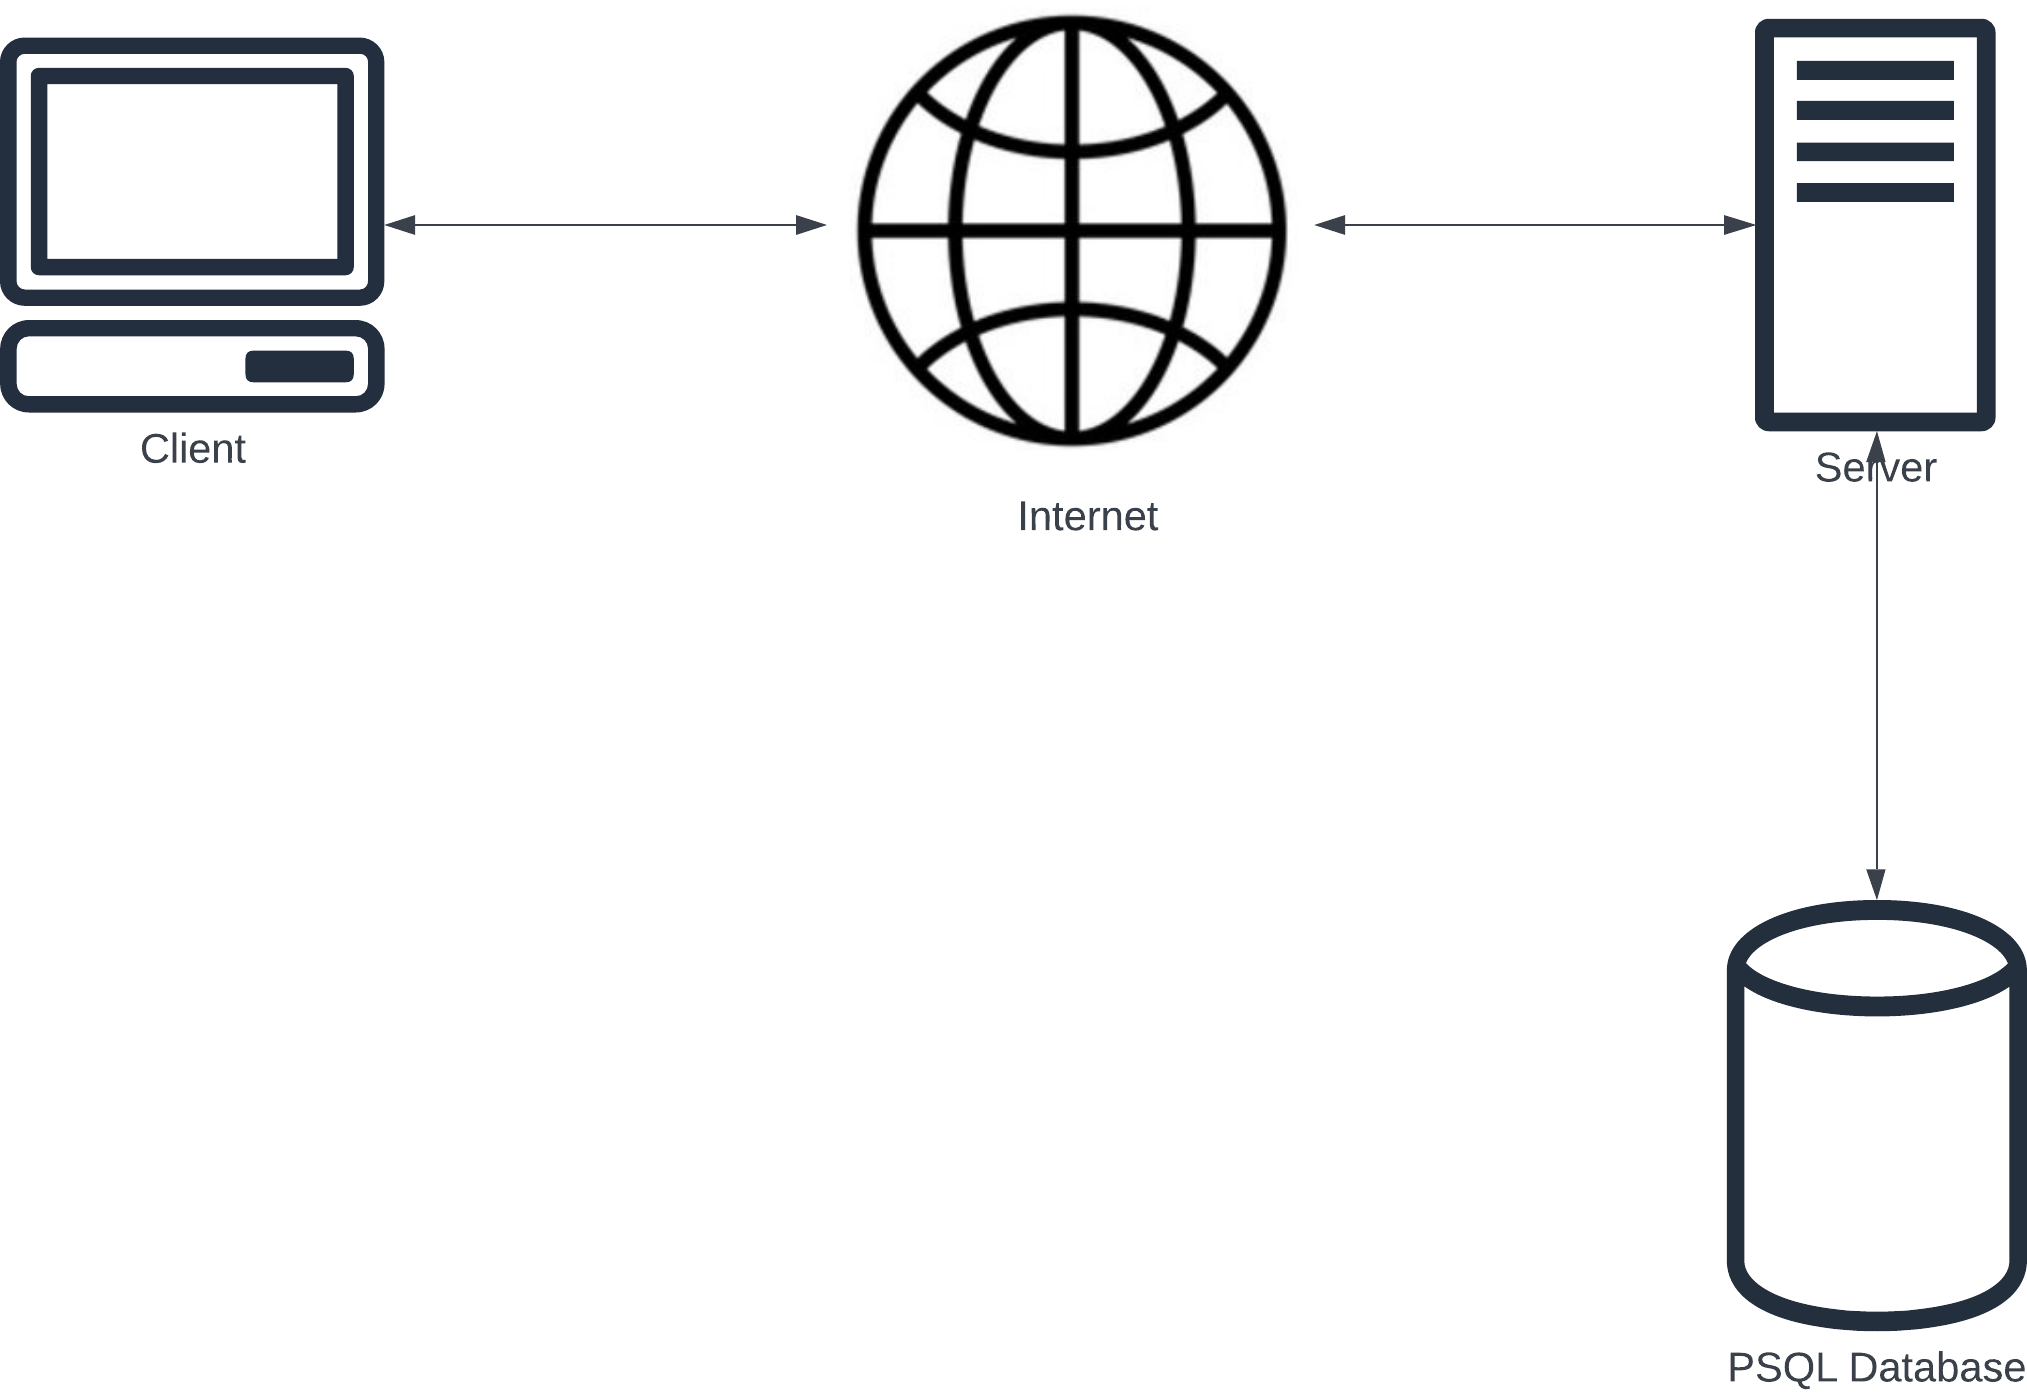
\includegraphics[width=250px]{figures/client-server.png}
  \caption{Client-Server Architecture}
  \label{fig:clientserver}
\end{figure}

\subsection{Database Design}
\label{system:database-design}

The database is a pivitol part of the artefact's extended functionality, it primarily servers as a hazard index database, whilst also storing different areas of concerning cycling infrastructure. PostgreSQL was chosen as the Relational Database Management System (RDBMS), as PostGIS was available to use to add the functionality for storing, indexing and querying of geospacial data (\cite{noauthor_postgis_nodate}). This data is used to display concerning areas on the map for which users may want to avoid, with the potential to include native routing support to avoid these hazards, futher highlighted under future work \see{evaluation:future} \see{fig:erd}. 

\begin{figure}[!ht]
  \centering
  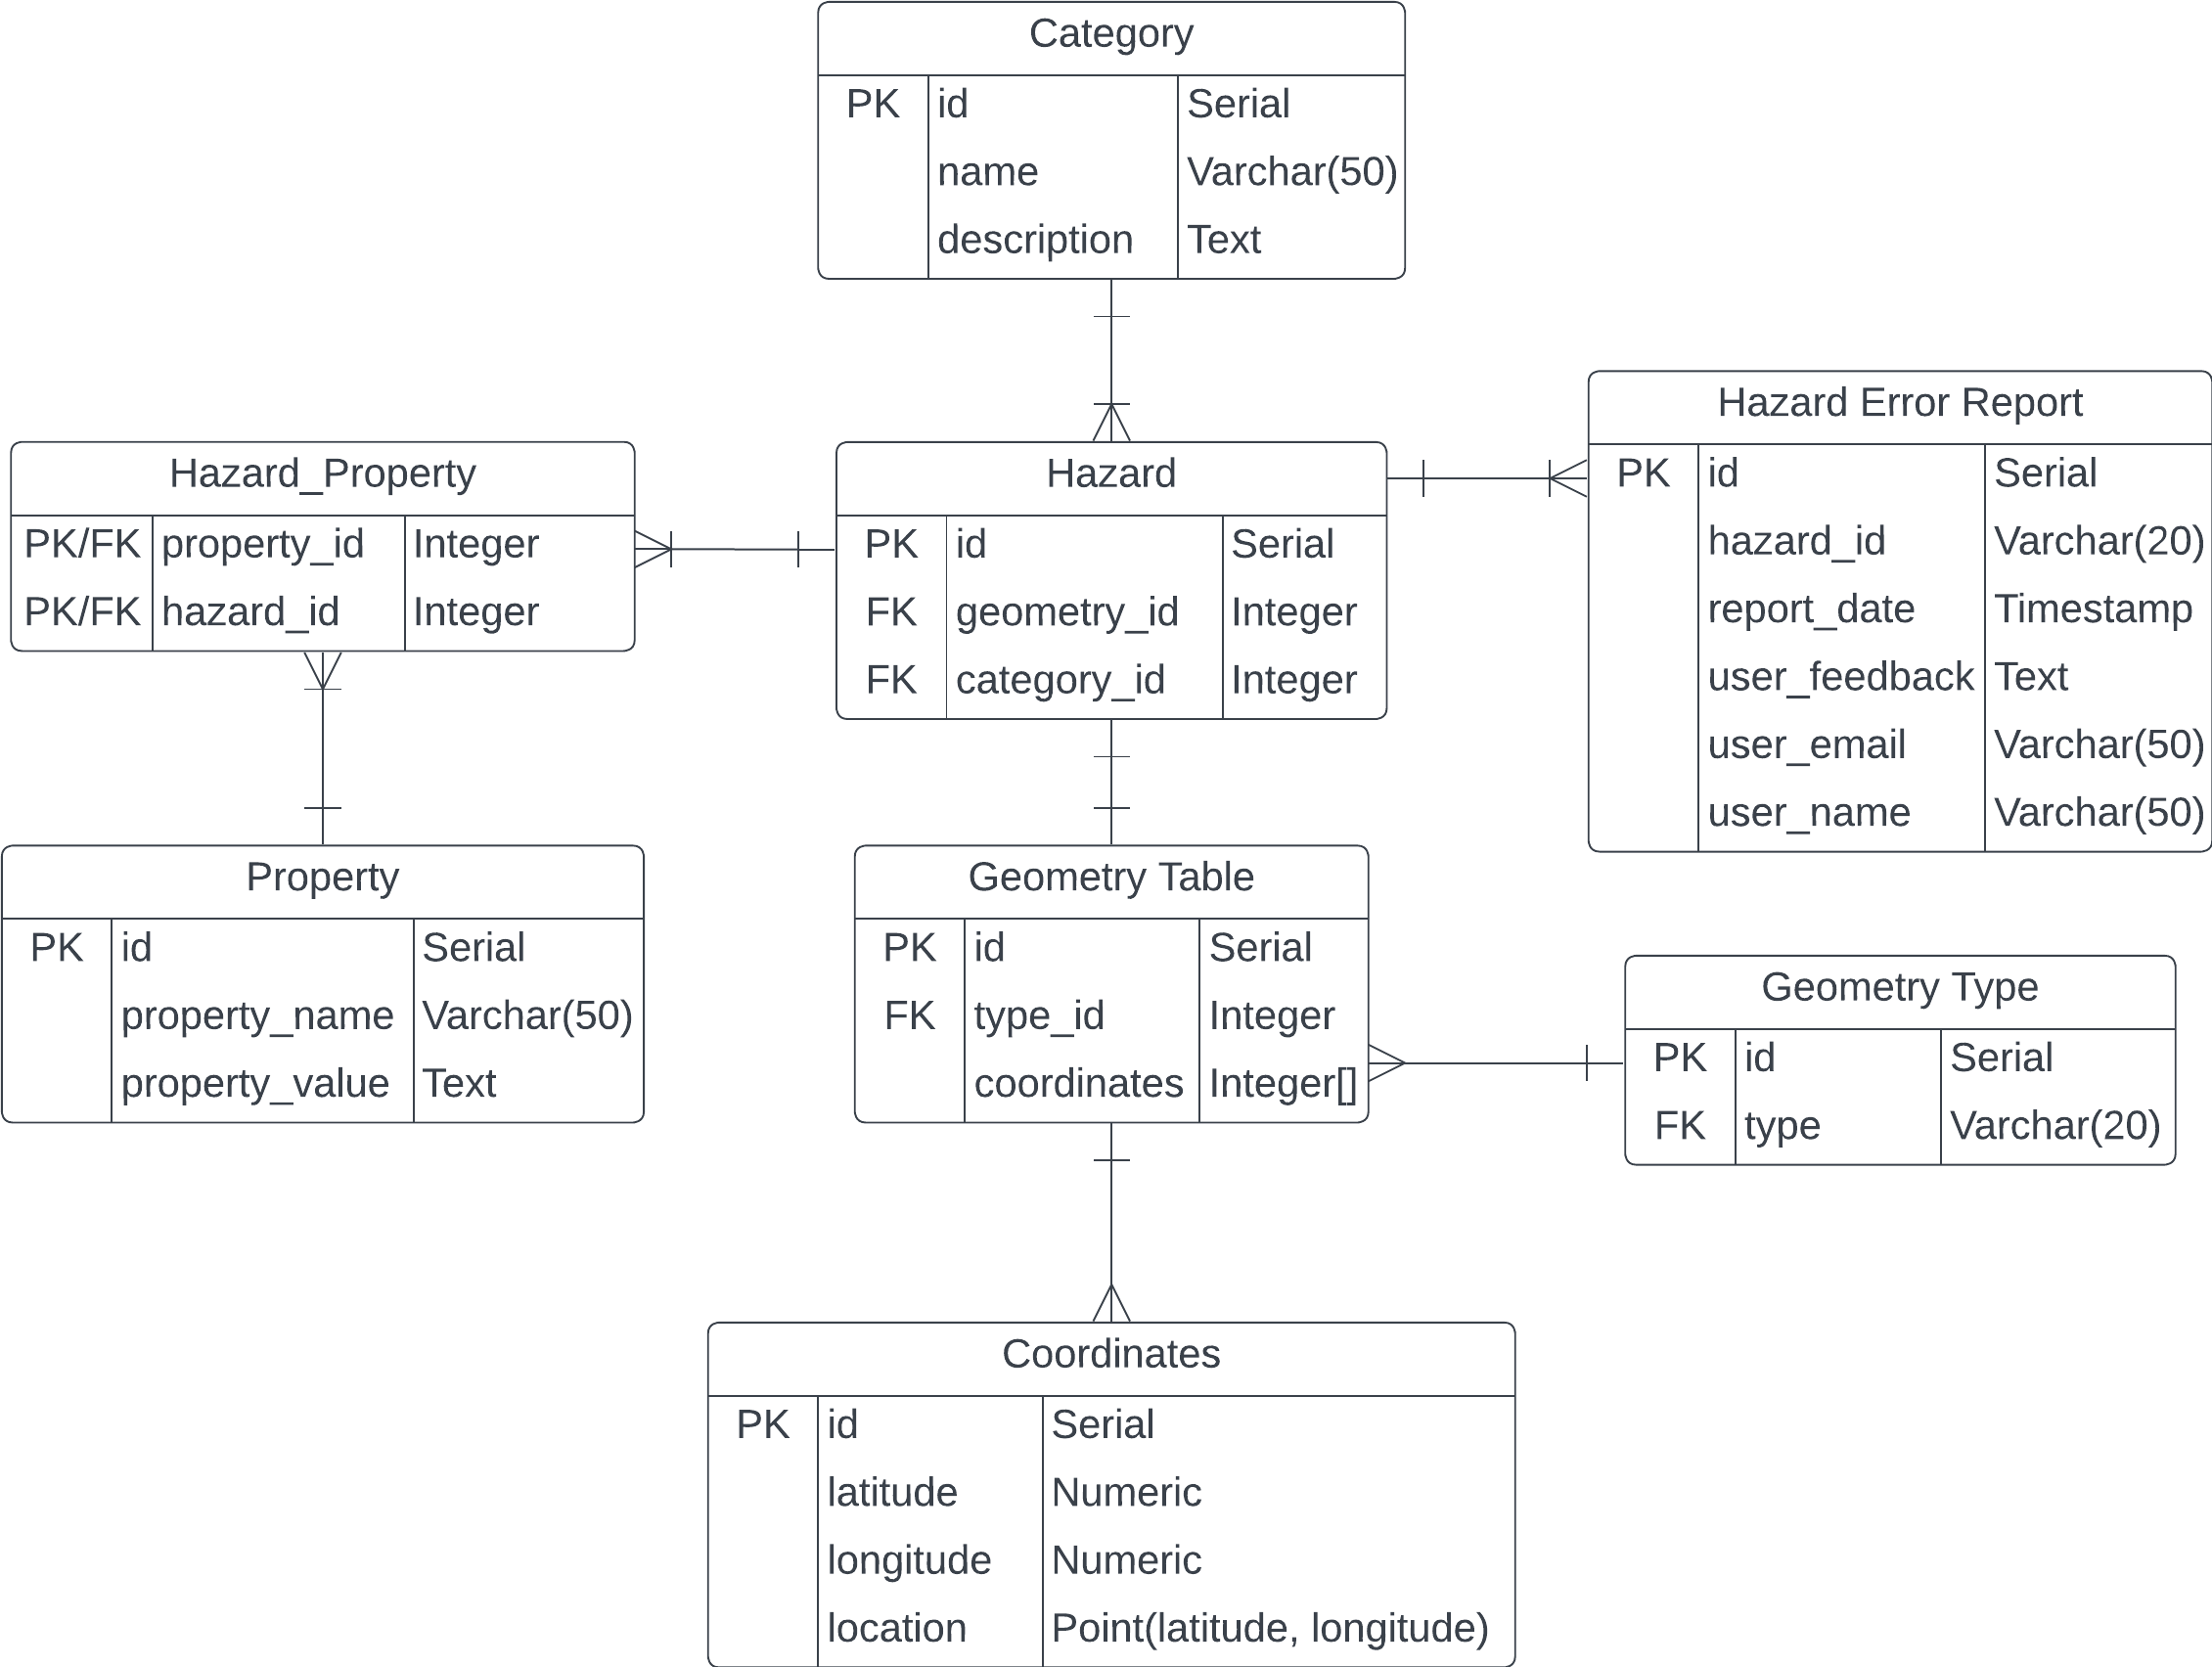
\includegraphics[width=350px]{figures/erd.png}
  \caption{Entity Relationship Diagram}
  \label{fig:erd}
\end{figure}

\subsection{Modular Architecture}
\label{system:modular-architecture}
React.js allows for a modular design approach utilising the component-based framework and storing variables in the form of states to re-render the application depending on the states of different variables. All the necessary data, functions and states can be passed to and from different components using the props functionality built into React, whereby a component inherits data from its parent component \see{fig:components}.

While the App.jsx file is the starting point of the React application, the Map component acts as the primary parent for most of the artefact's key components. Multiple states and variables are declared within Map and are transferred across the rest of its children via props, this is necessary, because all the key functionality of the route planner is wholly dependent on the Map component. However, not all child components of Map are required for the application to function, demonstrating the modular functionality of the application. The LeftPanel component and its children remain standalone from the rest of the application as these components act to display information, rarely updating.

\begin{figure}[!ht]
  \centering
  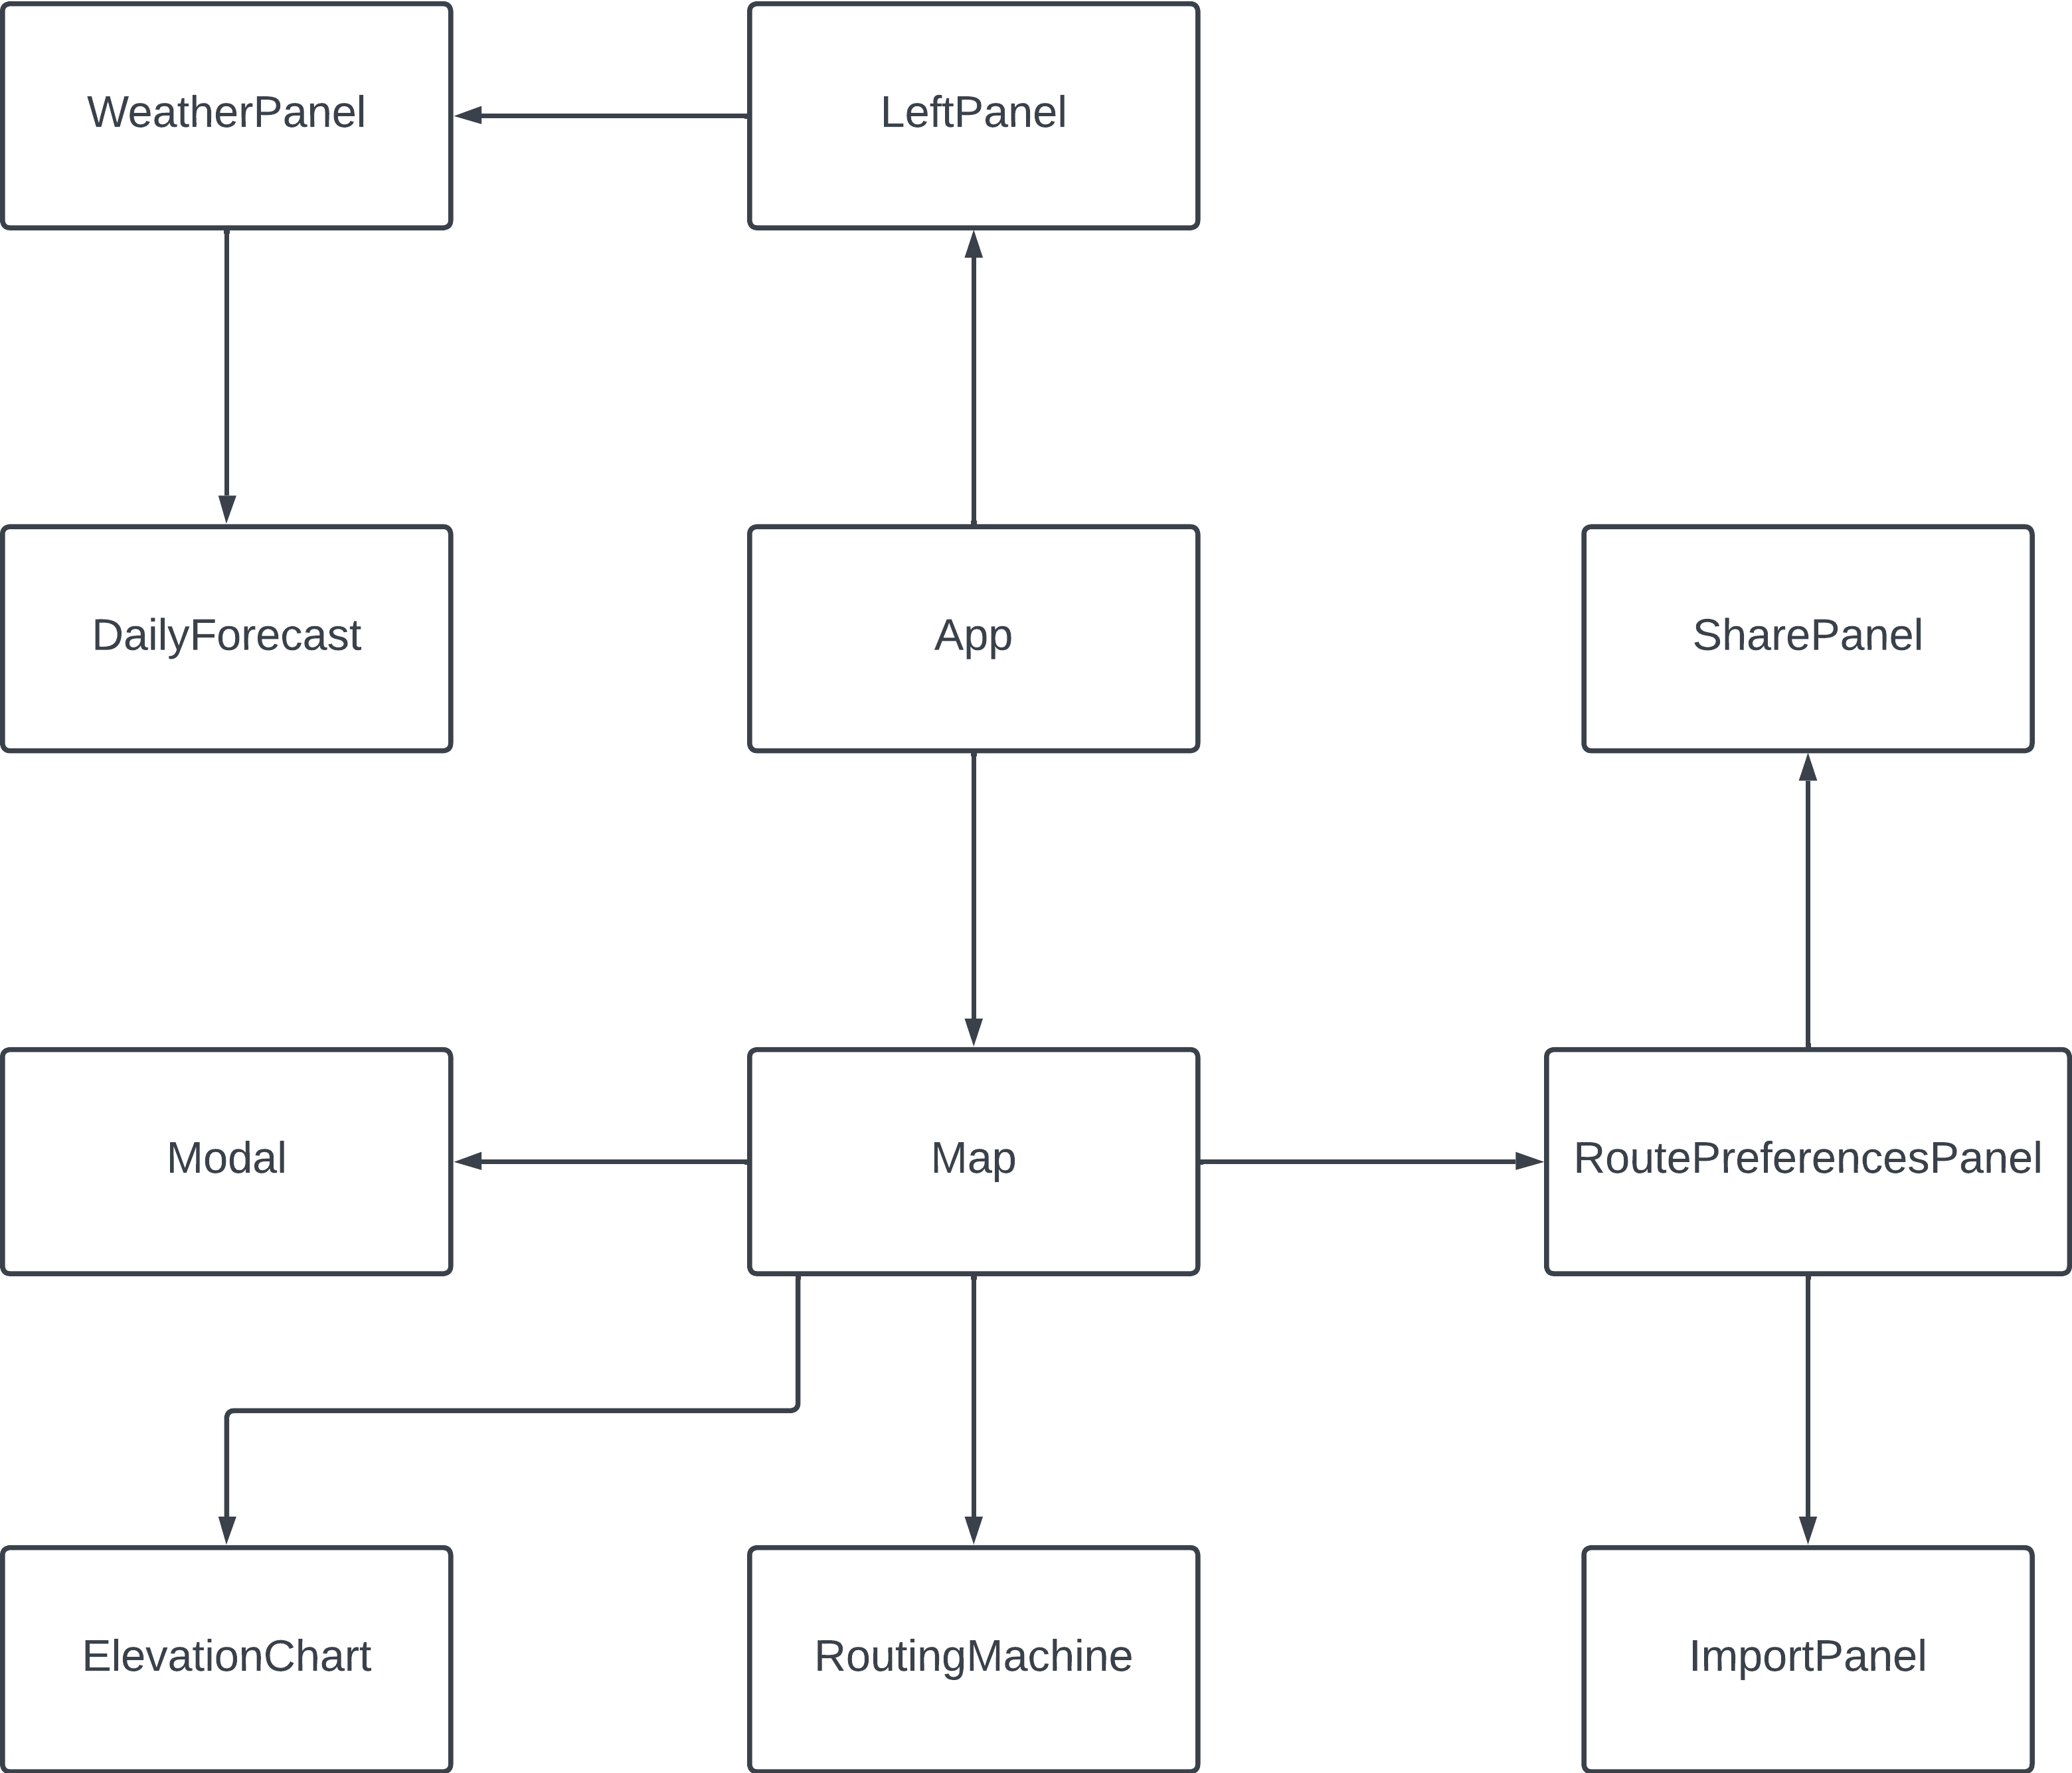
\includegraphics[width=400px]{figures/components.png}
  \caption{Modular Components}
  \label{fig:components}
\end{figure}

\clearpage
\section{Critique of Designs}
\label{design:critique}

The progressive approach was used to develop the UI, and whilst beneficial to the overall project and its aims, mobile devices were not catered for. While this can be seen as bad software development practice, the artefact is aimed at users on a desktop environment, exporting routes to external mobile navigation/fitness applications. Therefore, the designs were catered for a desktop experience, over a mobile-first design.

Both high-fidelity designs only demonstrate a light mode colour scheme. Due to this, all users are forced to use the artefact in a brighter, light mode with no option of customisability. In hindsight, it would have been beneficial to develop multiple high-fidelity designs to include both a light and dark mode for the artefact.

The database was designed to only store hazard and cycling infrastructure information, ideally, the database would store more than just this data. To expand some of the artefact's basic functionality, the database would also store user oAuth tokens, as well as their planned routes. Implementing such tables would enable the user to load more than just the last planned route into the application, without the requirement to store GPX/GeoJSON files locally, instead, they could save routes to their account. These tables would also enable a more expansive sharing functionality to social media, enabling users to share links to routes, rather than map screenshots of their routes \see{evaluation:future}.

Finally, the modular architecture approach, was ideal for developing the artefact, however, the modules could have been better structured to maximise the benefits of the modular approach. The artefact should be customisable, whereby specific modules can be disabled entirely if the user doesn't require them. At this stage, the design only caters to the manual disabling of each module, with certain modules being necessary for the artefact to function \see{evaluation:limitations}.
\chapter{Implementation}
\label{chap:implementation}

This section describes the artefact development process. Despite multiple stumbling blocks during development, these were overcome through problem-solving, thorough investigation and reading of software documentation.  

\section{Development Environment}
\label{implementation:de}

Visual Studio Code (VS Code) was chosen as the development environment for development (\cite{noauthor_visual_nodate}). VS Code was chosen due to its flexibility in working with multiple programming languages through the use of extensions. The React.js Framework, JavaScript and Go Language extensions were installed to ensure seamless development of the backend and frontend of the artefact. The ESLint extension was also used using Go and JavaScript configurations to ensure the consistency and readability of the codebase.

\section{Iteration 1 - Basic UI and Core Routing}
\label{implementation:iteration1}
The initial stages of development began using a first draft of elicited requirements \see{appendix:initial-user-requirements} where later in the project, a new set of user requirements was formed based on primary research. This method proved effective in not delaying initial development, where the core requirements were unlikely to change greatly. Furthermore, Iteration 1 consisted of implementing the building blocks of the artefact, including setting up a React.js App, Gin Webserver, PostgreSQL database and the core routing functionalities.

\subsection{Leaflet - Open Street Map (OSM)}
\label{iteration1:leaflet-osm}
The Map component was the first to be developed because the rest of the artefact would be dependent on its mapping functionality. The component contained a div element containing the MapContainer component imported from React Leaflet (\cite{noauthor_react_nodate}). The component includes a tile layer to make API requests to Open Street Map (\cite{noauthor_openstreetmap_nodate}) to get the tile images for the map, and then display these tiles to form the full-screen map element. Temporary variables were set up to store the latitude and longitude values representing the start and end of a route, then drawn on the map using a polyline and marker points \see{fig:basic-map-with-route}. 

\begin{figure}[!ht]
    \centering
    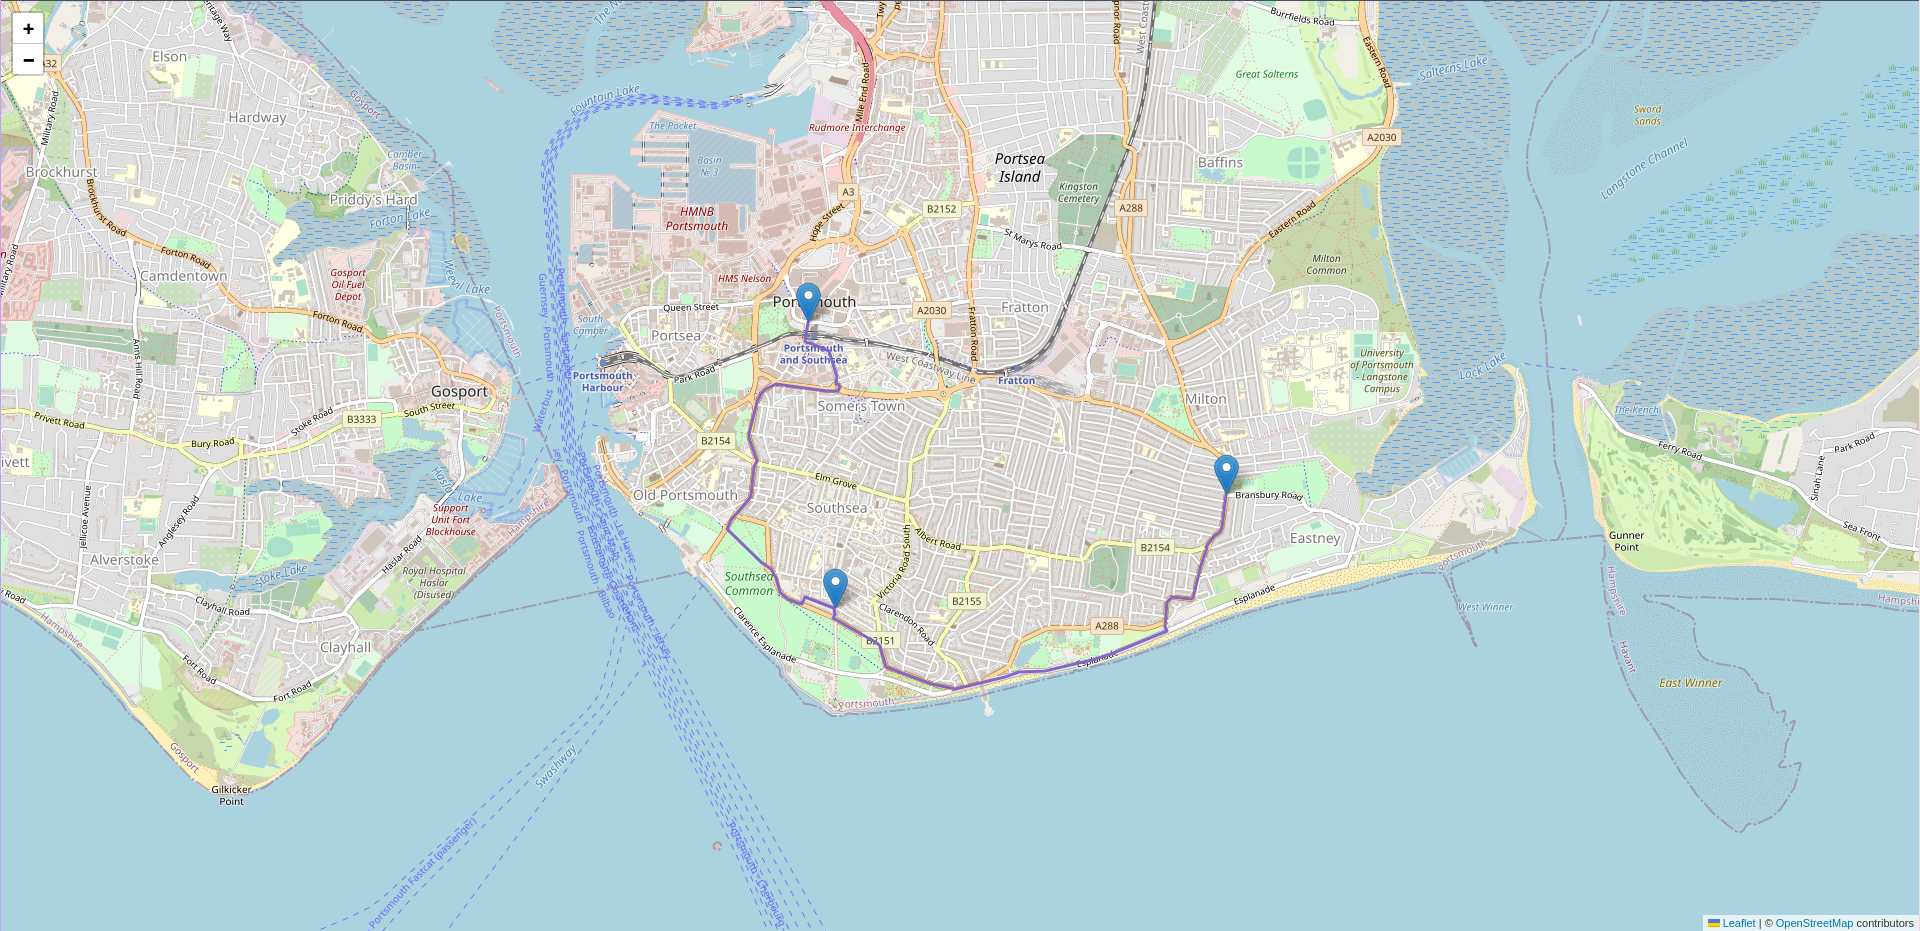
\includegraphics[width=425px]{figures/Progress Images/Iteration-1/SR25/Basic Route.png}
    \caption{Basic Map with Route}
    \label{fig:basic-map-with-route}
\end{figure}

\subsection{Basic Route Planning}
\label{iteration1:basic-routing}
After conducting research, the most effective way to implement route planning with Leaflet was to use Leaflet Routing Machine (\cite{noauthor_leaflet_nodate-1}). This library enabled a RoutingMachine component to be natively added on top of the React Leaflet map component, whilst providing a basic, customisable route planning UI \see{fig:routing-ui}. The routing API in use at the beginning was Open Source Routing Machine (OSRM) (\cite{noauthor_project_nodate}) which appeared to meet all requirements of a routing algorithm until round trip routing was required \see{implementation:iteration2}. This new routing functionality enabled the user to select a start, destination and any intermediate locations, a route would then be planned. At this stage, the route could be altered through the use of waypoints, but the artefact did not provide any further custom routing features to the user.
\begin{figure}[!ht]
    \centering
    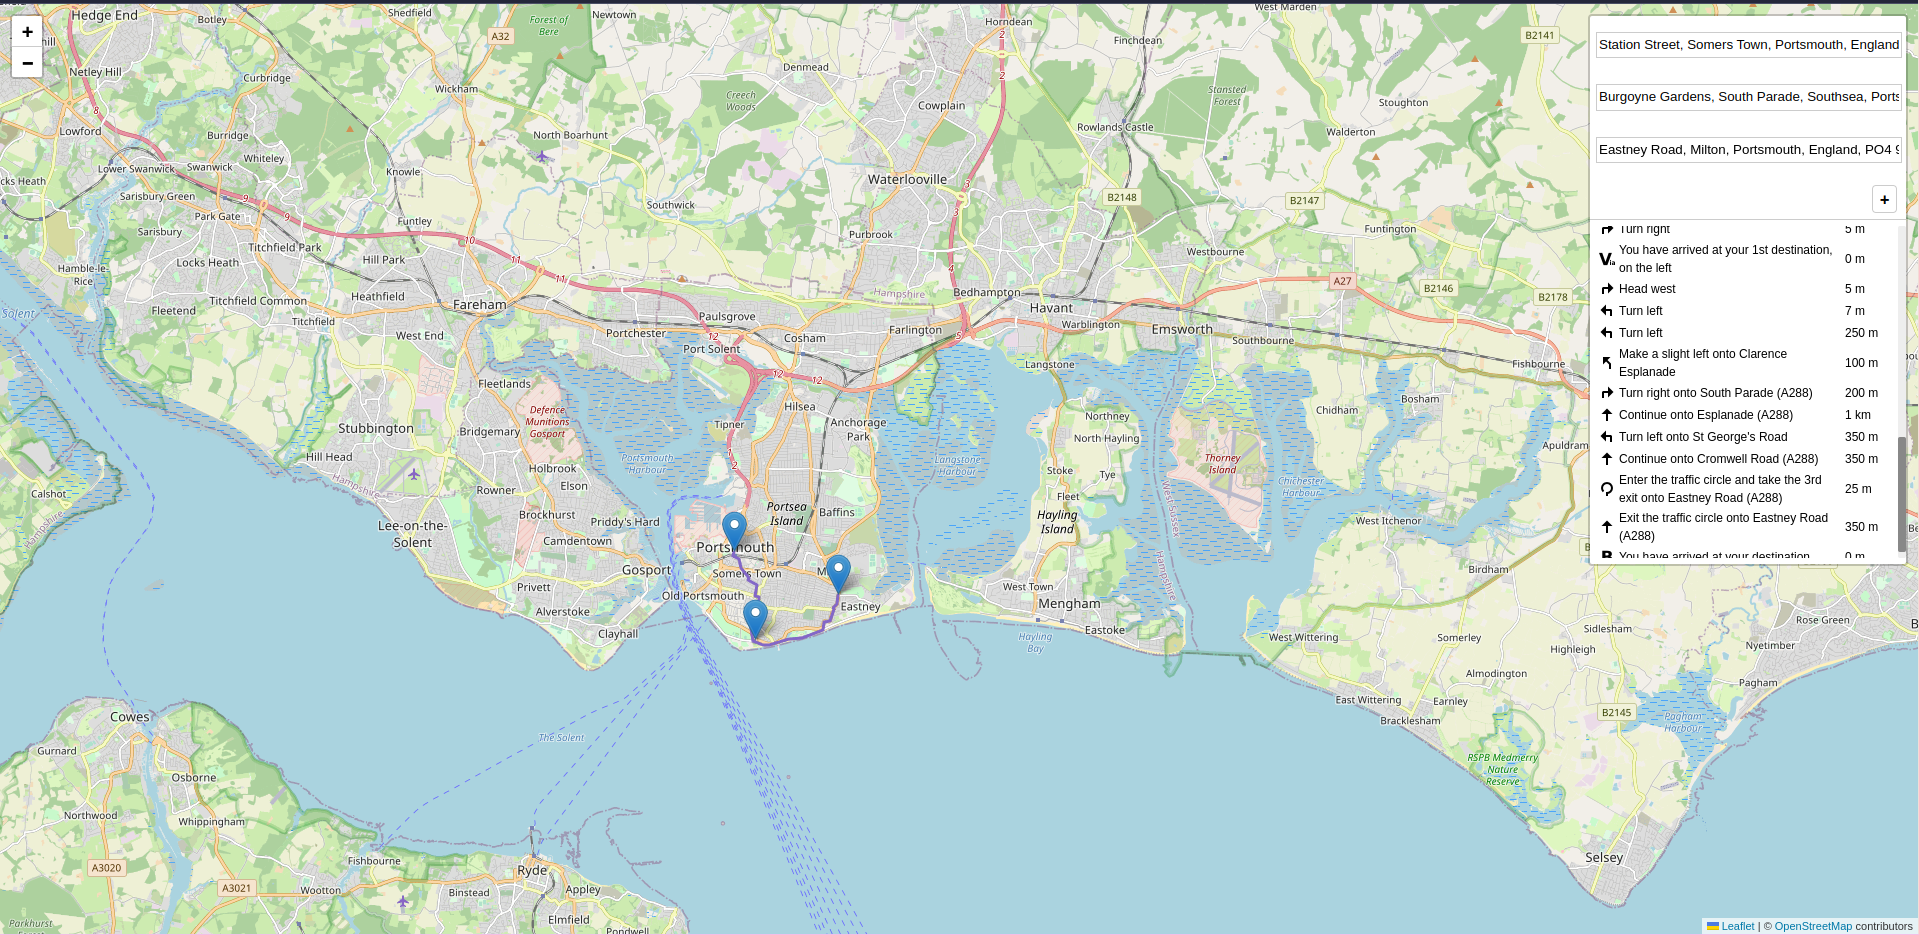
\includegraphics[width=425px]{figures/Progress Images/Iteration-1/SR1/Basic Destination Overlay Set up.png}
    \caption{Routing UI}
    \label{fig:routing-ui}
  \end{figure}

\subsection{Elevation Chart}
\label{iteration1:elevation-chart}
To create an elevation chart, the component was declared, with the plan to use Chart.js (\cite{noauthor_chartjs_nodate}) to draw the plot on a canvas element. A div was created to hold the chart component, where the elevation data was gathered from a state variable called 'coordinates' which contained the route latitude, longitude points and the altitude/elevations for each point \see{fig:waypoint-arr}. The distance along the route for each elevation point is calculated by dividing the total route distance (taken from a state variable called 'summary') by the length of the 'coordinates' array. To ensure continuity between the map and the elevation plot, a simple feature was added to allow the user to hover over the elevation plot, with the matching point along the route being highlighted. This required the hover point on the chart's canvas element to be found, matching the hover value to the latitude and longitude with the respective point and drawing a circle element on the Leaflet map \see{fig:elevation-hover}.

\begin{figure}[!ht]
    \centering
    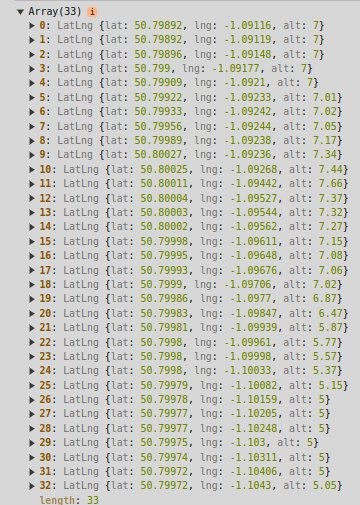
\includegraphics[width=200px]{figures/Progress Images/Iteration-1/SR1/waypoint-arr.png}
    \caption{Route Waypoint/Elevation Array}
    \label{fig:waypoint-arr}
  \end{figure}

\begin{figure}[!ht]
    \centering
    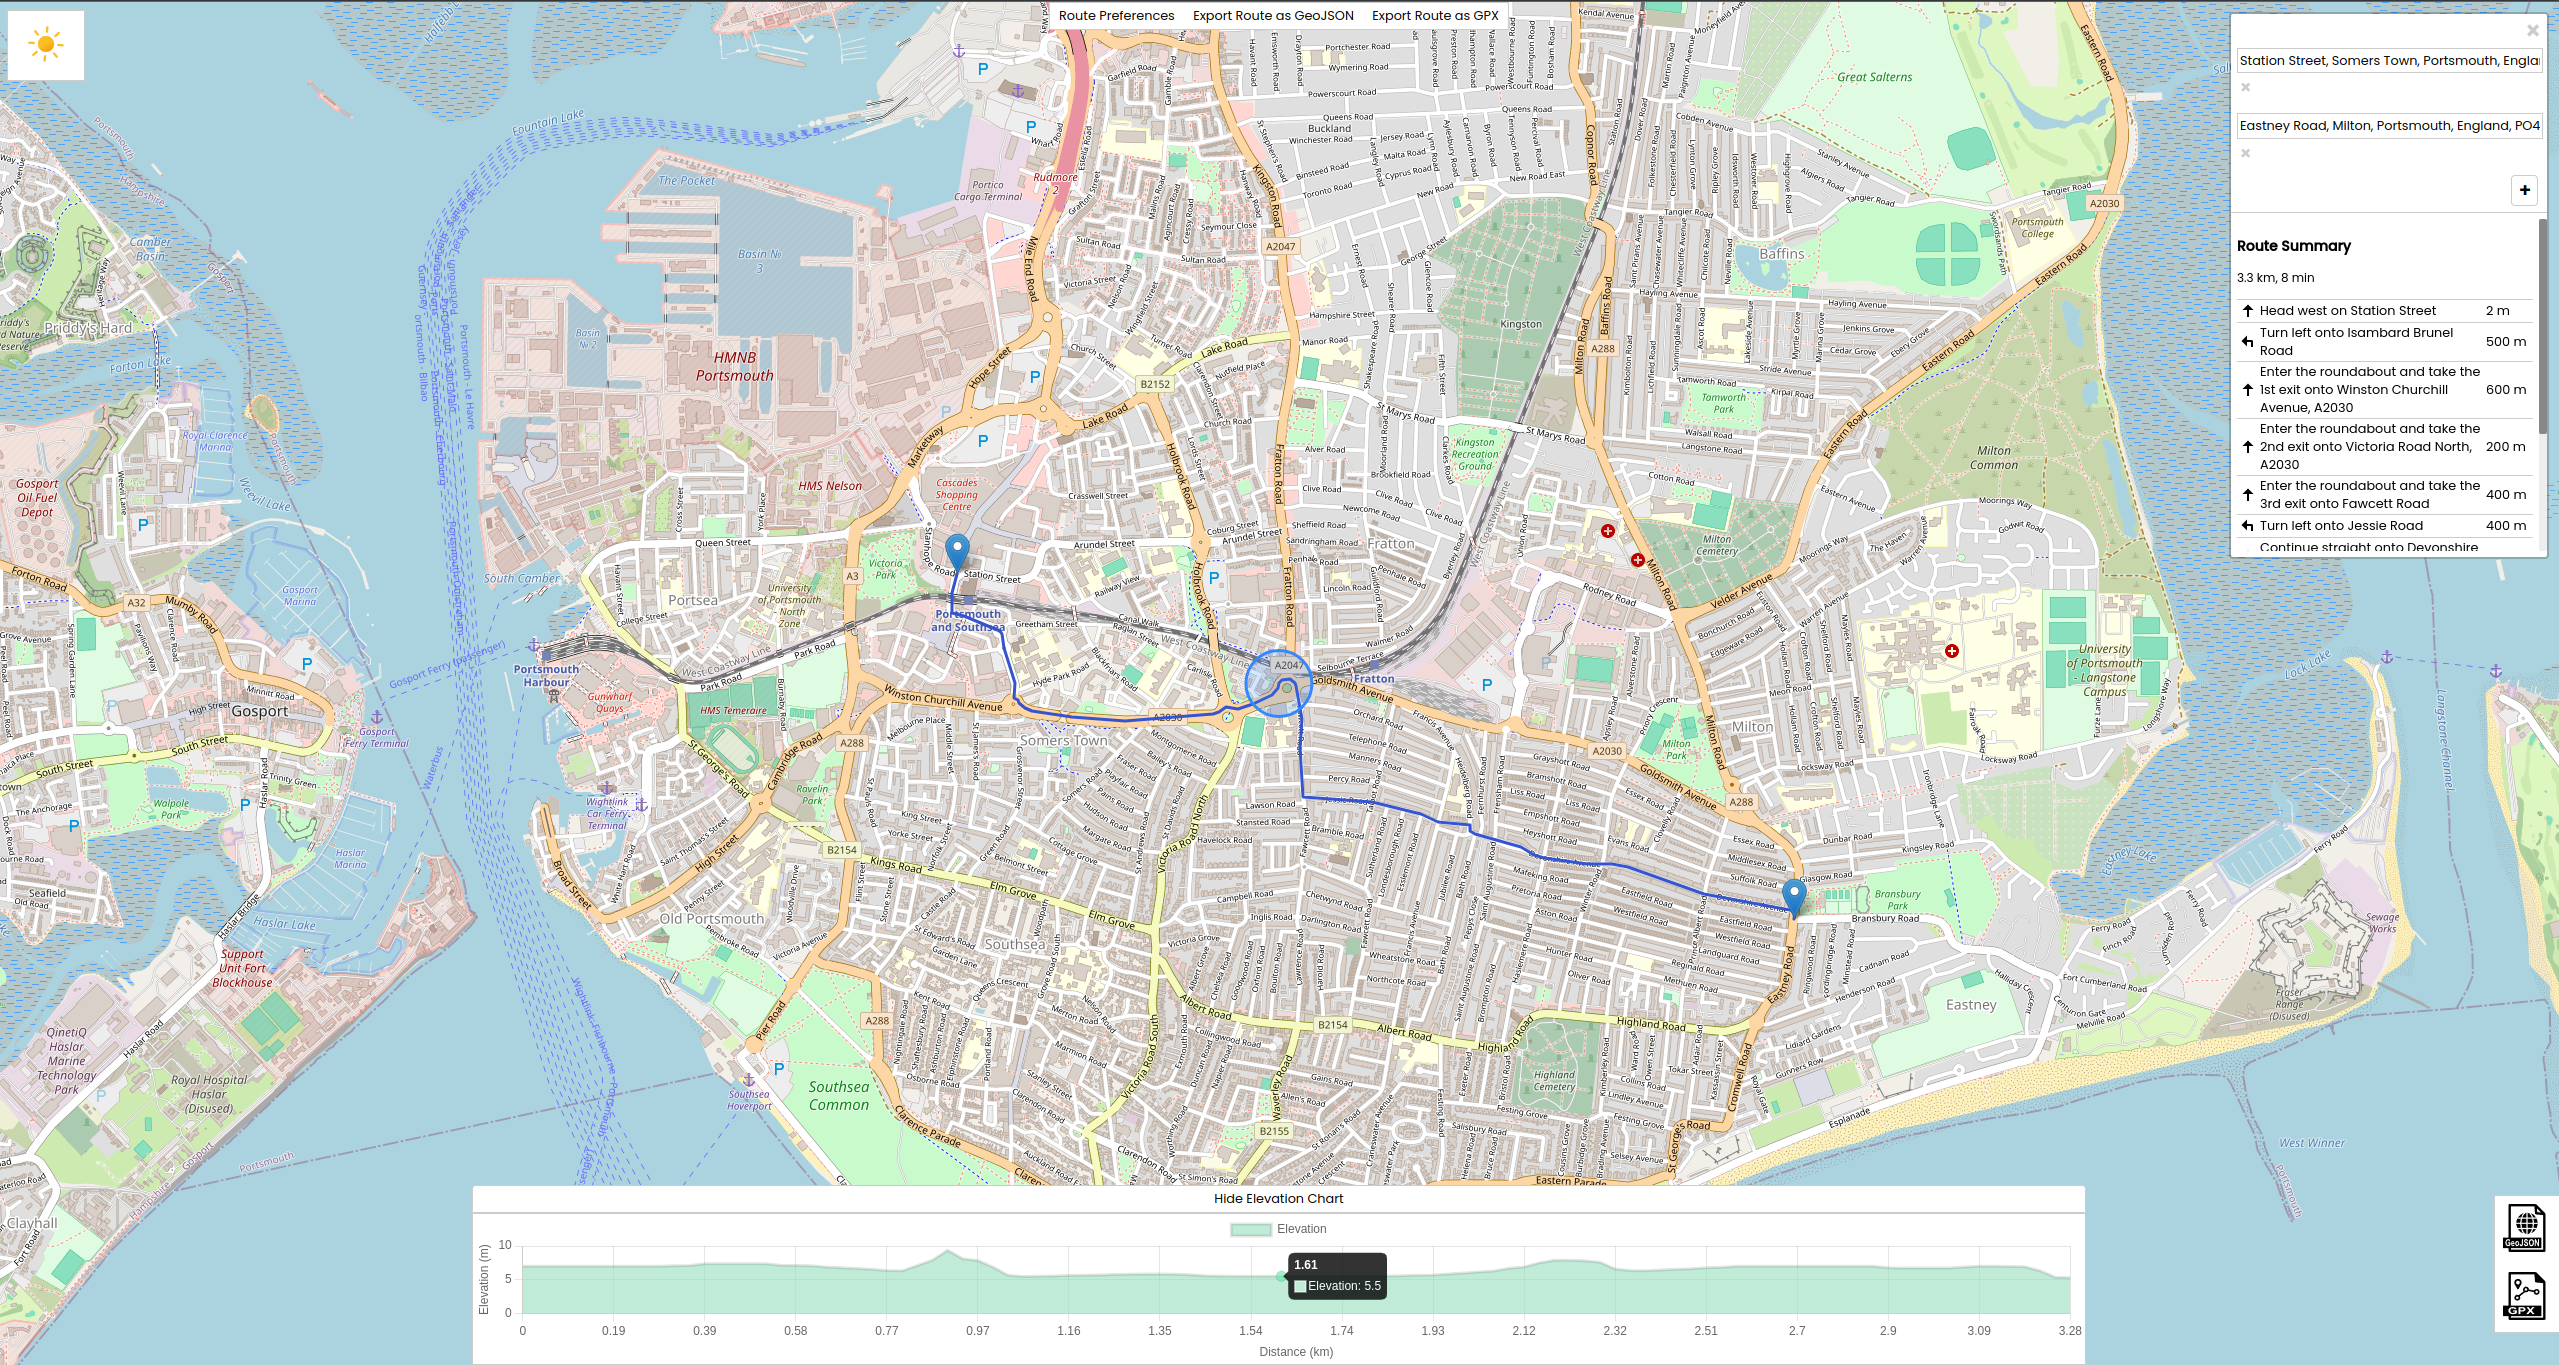
\includegraphics[width=425px]{figures/Progress Images/Iteration-1/SR28/elevation-hover.png}
    \caption{Elevation Plot Hover Functionality}
    \label{fig:elevation-hover}
\end{figure}

\subsection{Weather Information Panel}
\label{iteration1:weather-panel}
A generic weather panel was created within iteration 1, displaying weather information for the current day at the user's current location. The weather panel used the browser's geolocation API called within a React useEffect to get the user's general location, asking for permission via a pop-up window, then storing the geolocation in a state variable. The approximate coordinates returned from the API were then passed to Open Weather Map to gather all weather data for the current day. The Meteocons icons (\cite{noauthor_weather_nodate}) were used to display images demonstrating the current weather conditions \see{fig:basic-weather-panel}. The visibility of the weather panel was determined by a State variable, if the variable was true, the height and width of the panel expand, and when false, reduce to the button size.

\begin{figure}[!ht]
    \centering
    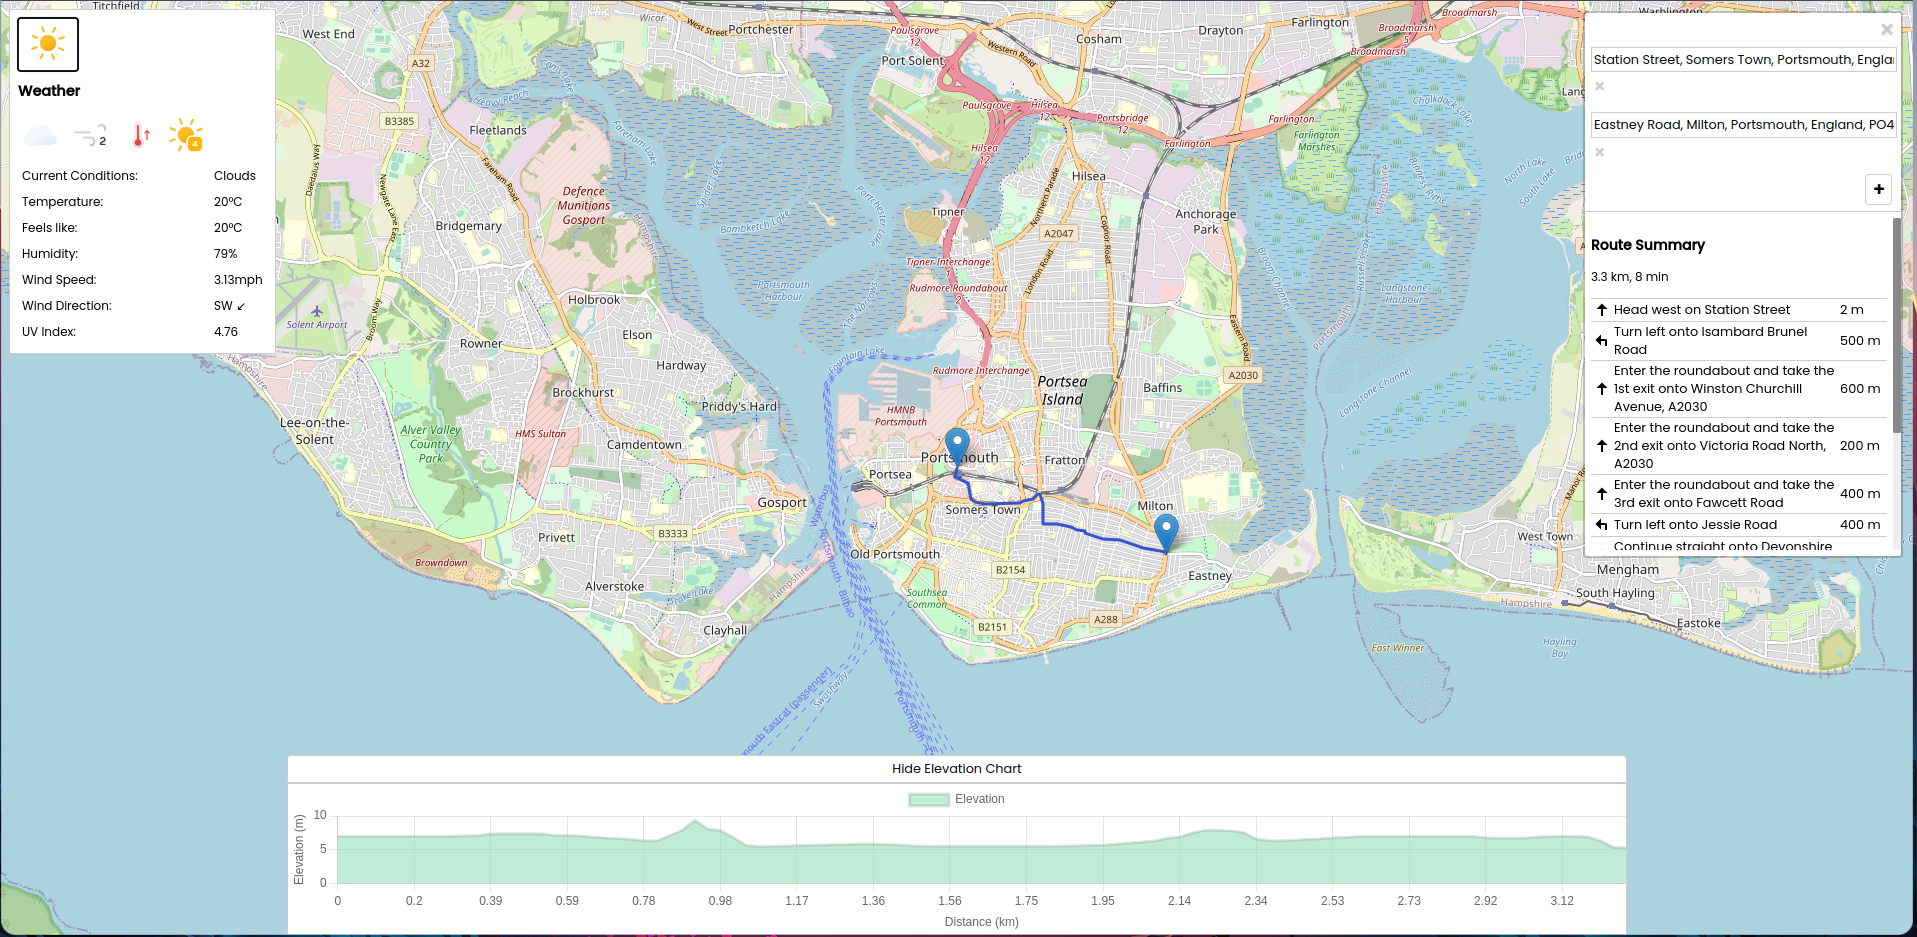
\includegraphics[width=300px]{figures/Progress Images/Iteration-1/SR19&SR28 Combined/SR19&SR28 Merged.png}
    \caption{Weather Panel}
    \label{fig:basic-weather-panel}
\end{figure}

\subsection{Main Challenges}
\label{iteration1:main-challenges}
The main challenge of Iteration 1 (i1), was primarily integrating multiple services to communicate seamlessly through the React.js frontend. Syncing hovering over the elevation plot, with a matching point along the route polyline, proved difficult. Despite the calculations being simple to determine at what latitude and longitude to draw the circle marker on the map when hovering on the plot, getting the map instance reference was more difficult than expected. Initially, the reference would return undefined, therefore no marker was drawn on the map, however after implementing a useState and declaring a local copy of the map instance, the hover functionality worked seamlessly.

Furthermore, the only other challenge faced was retrieving the user's geolocation from the browser. A useEffect was required to access the geolocation API, however, the useState was at first missed to store the geolocation value once the API had returned the data. Once the state variable was added, however, the weather panel would re-render once the data was retrieved.

\section{Iteration 2 - Route Sharing, Hazard Index and POI Integration}
\label{implementation:iteration2}

Unlike i1, Iteration 2 (i2) development was conducted after the primary research and requirements review had been completed. The remaining updated requirements were prioritised and distributed between i2 and Iteration 3 (i3) \see{implementation:iteration3}. I2 builds on i1, enhancing existing functionality and introducing new features throughout the iteration. 

\subsection{Sharing Route Functionality}
\label{iteration2:sharing-route}

Route sharing was implemented with i2, when routes were found using Open Route Service, GPX (\cite{noauthor_gpx_nodate}) and GeoJSON (\cite{noauthor_geojson_nodate}) strings were generated. These files were then used to create a share to email feature using the Twilio SENDGRID API (\cite{noauthor_email_nodate}). Initially, it was planned to send emails direct to the SENDGRID directly from the client, to mitigate the middle-man required to send the request, however it was found that SENDGRID would only accept incoming requests from the server. Therefore, an API endpoint was created with Gin to handle the POST request from the frontend. 

Each email would contain a simple amount of predefined text with the included GPX and/or GeoJSON files selected for export. A modal was created to display the email form, where the user could input the recipient's email address, route name and choose what type of file to share \see{fig:basic-weather-panel}.

Initially, it was planned to use the Strava API to upload GPX files directly to the user's Strava Routes account, however, it was found that the Strava API had no such endpoint to integrate with routes. It was decided to still implement Strava integration, but with activities, enabling route export as an activity for users without dedicated fitness devices. 

A modal was created \see{fig:strava-modal} and a POST request endpoint set up to handle the request to the Strava API. The user would be required to log in to their Strava account, to enable the artefact access to upload activities. Once logged in, the user could select the route to upload, then the artefact would send the GPX file to the Strava API, where it would be converted to an activity and stored in the user's account \see{fig:strava-example}.

\begin{figure}[!ht]
  \centering
  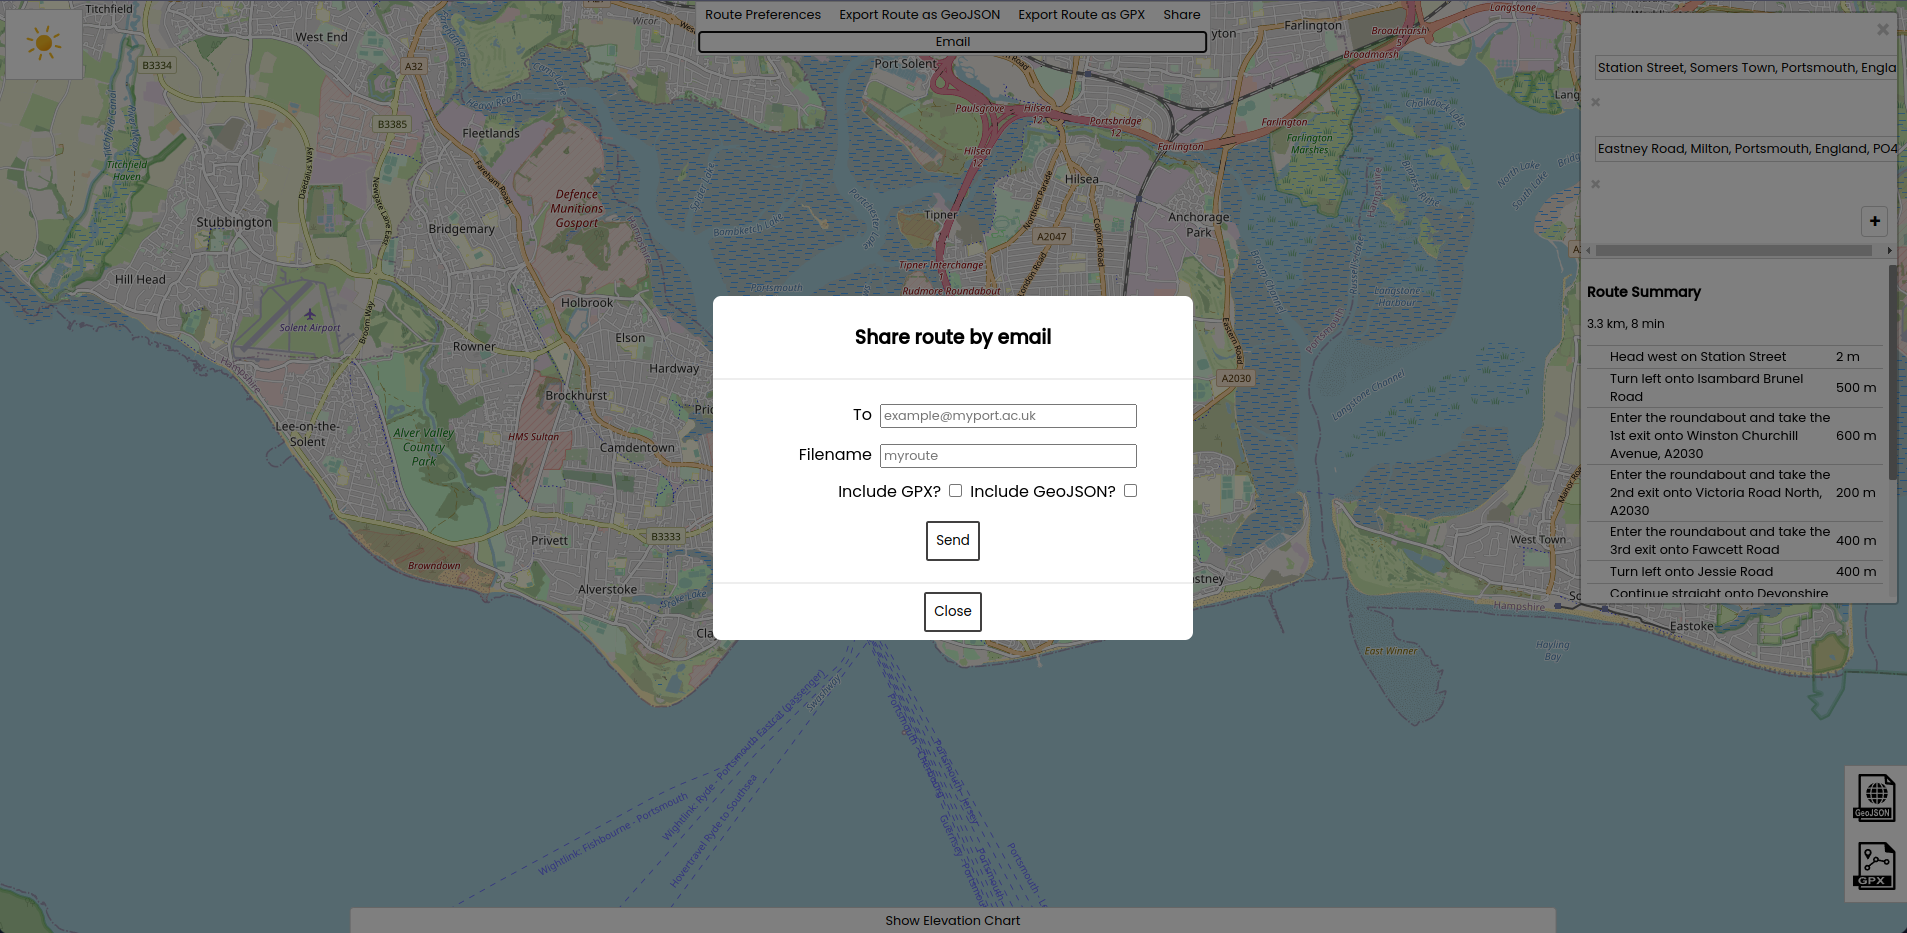
\includegraphics[width=425px]{figures/Progress Images/Iteration-2/SR17/SR17png.png}
  \caption{Share to Email Modal}
  \label{fig:share-email-modal}
\end{figure}

\begin{figure}[!ht]
  \centering
  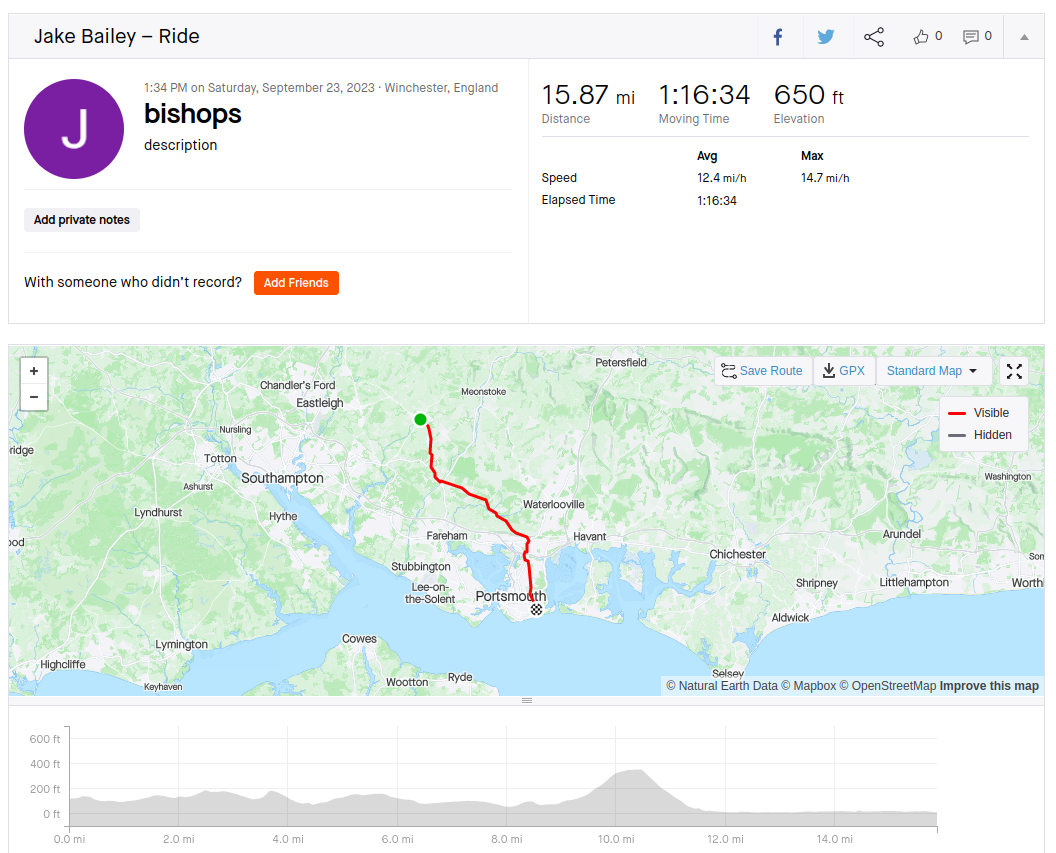
\includegraphics[width=425px]{figures/Progress Images/Iteration-2/SR18/SR18 Upload Example 1.png}
  \caption{Strava Activity}
  \label{fig:strava-example}
\end{figure}

\begin{figure}[!ht]
  \centering
  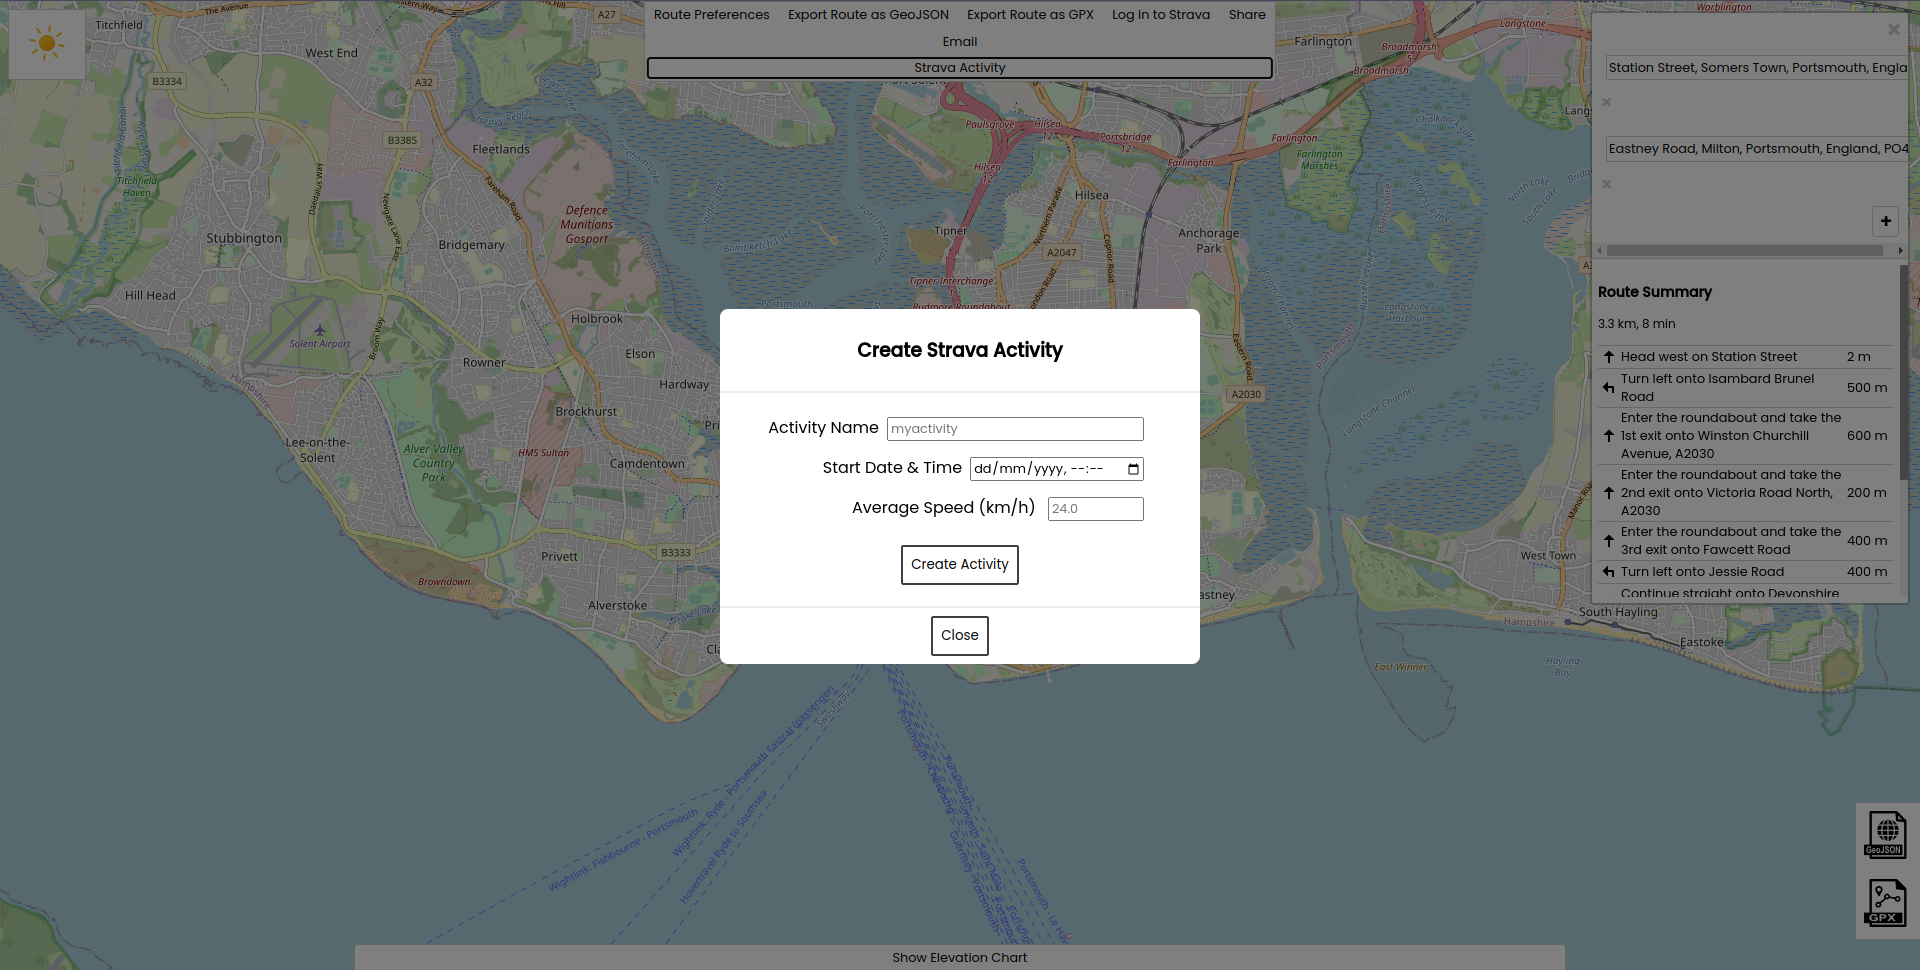
\includegraphics[width=425px]{figures/Progress Images/Iteration-2/SR18/SR18 Strava Modal.png}
  \caption{Share to Strava Modal}
  \label{fig:strava-modal}
\end{figure}


\subsection{Hazard Index Database Creation and Integration}
\label{iteration2:hazard-index}

Creation and integration of the hazard index database was the largest task of i2. The database was created using PostgreSQL using PostGIS. The database was split into eight tables representing a hazard, related details and its geospatial data \see{system:database-design}. Hazard types were chosen based on the most relevant hazards defined on the Open Street Map wiki (\cite{noauthor_keyhazard_nodate}) with the addition of a 'Cycling Infrastructure' hazard. The 'Cycling Infrastructure' hazard type was added to allow users to report and view bad cycling infrastructure in their area, with the intention of routing algorithms avoiding these areas in the future.

To integrate the database into the artefact, API endpoints were created to handle GET and POST requests to the database. The database was connected to the Go backend using the 'github.com/lib/pq' package (\cite{noauthor_pq_nodate}), with Gin handling the routing of requests to the database. Using the fetch API, the frontend could make API calls, to add and retrieve hazards from the database, supplying coordinates for the hazard location/area and the hazard type \see{fig:hazard-creation}.

To enable users to contribute to the hazard index database, a UI was created using the Leaflet Draw API (\cite{noauthor_leaflet_nodate-2}). The API allowed a few controls to be added to the map, including buttons to draw markers and polygons onto the map. These buttons were used to create a hazard, where I implemented an event handler to catch the polygon/marker drawn once completed. This event handler would then proceed to make open the hazard creation modal, with the coordinates of the drawn polygon/marker passed to the modal via props. The user could then add the extra information required for the hazard and submit the hazard to the database.

Furthermore, to display the hazard data on the map, a new layer must be created. The layer was added to the map using the React Leaflet library, where the hazards were retrieved from the database and drawn on the map. These hazards were shown as both markers and polygons to represent a point or area hazard \see{fig:hazard-layer}. The API endpoint was set up to allow the user to retrieve all hazards within a five mile radius of a point, to enable the user to see hazards in their area, as the map was panned, the hazard layer would update \see{fig:hazard-API}.

\begin{figure}[!ht]
  \centering
  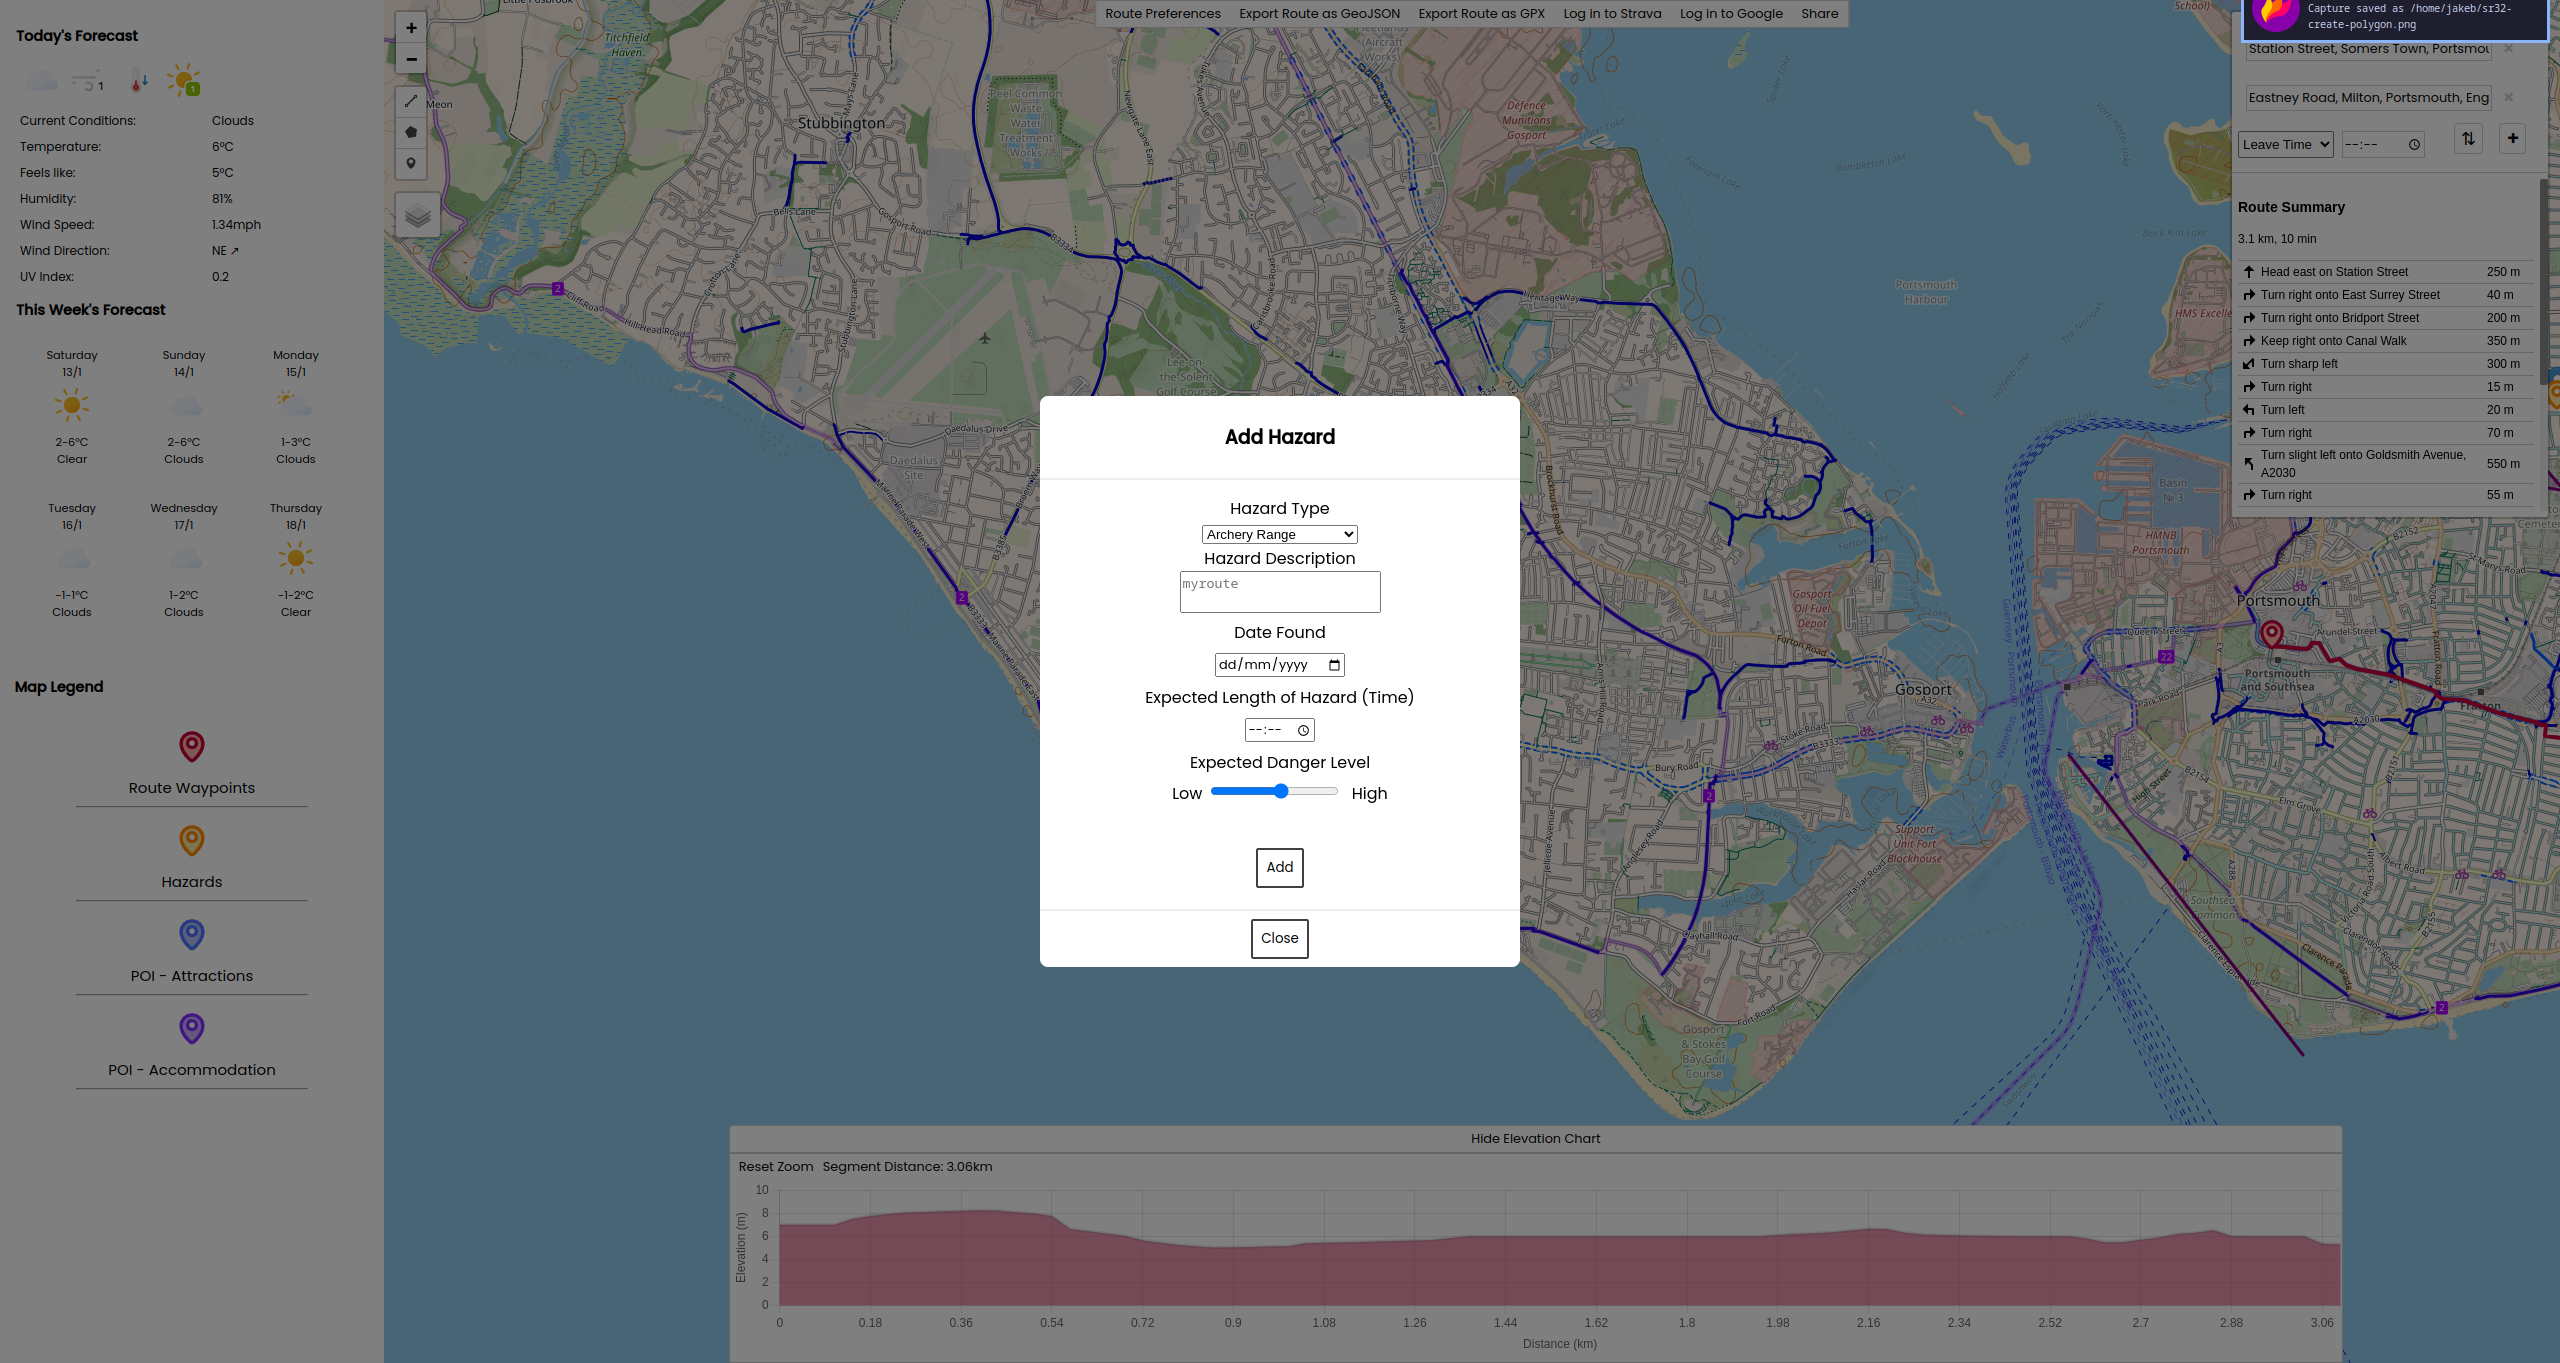
\includegraphics[width=425px]{figures/Progress Images/Iteration-2/SR32-37/sr32-add-hazard-point.png}
  \caption{Hazard Creation Modal}
  \label{fig:hazard-creation}
\end{figure}

\begin{figure}[!ht]
  \centering
  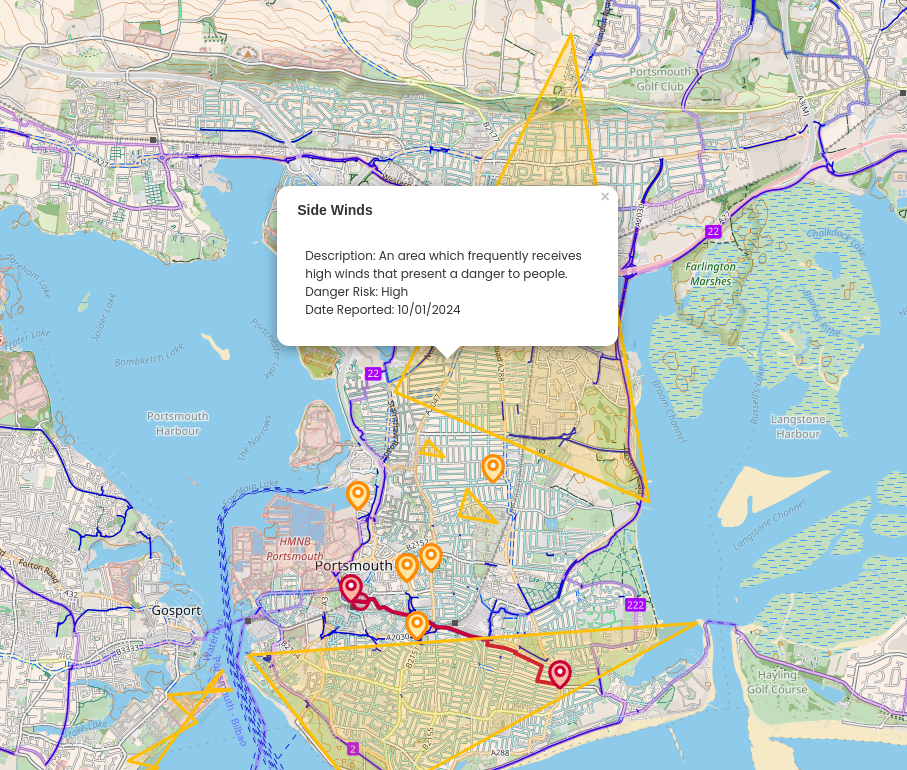
\includegraphics[width=300px]{figures/Progress Images/Iteration-2/SR32-37/sr32-hazard-popup.png}
  \caption{Hazard Map Layer}
  \label{fig:hazard-layer}
\end{figure}

\begin{figure}[!ht]
  \centering
  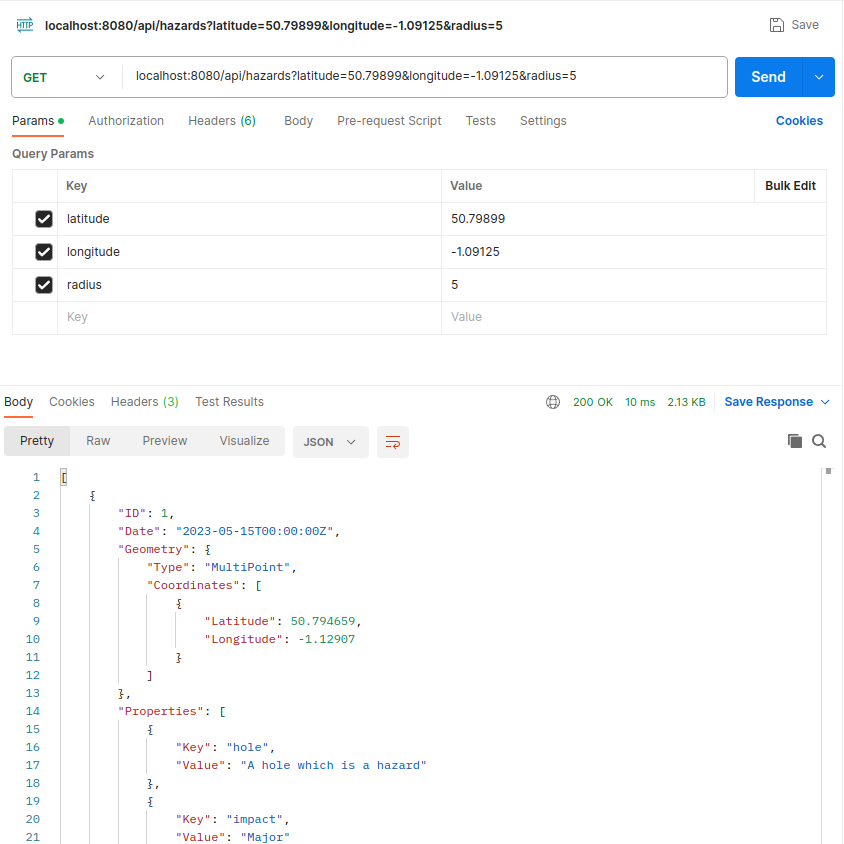
\includegraphics[width=425px]{figures/Progress Images/Iteration-2/SR32-37/SR32 - Basic API further developed.png}
  \caption{Hazard API Query}
  \label{fig:hazard-API}
\end{figure}

\subsection{Key Point-of-Interest (POI) Integration}
\label{iteration2:poi-integration}

The POI integration was the final feature of i2, where the user could view points of interest in their area. The POI data was retrieved from the Foursquare Places API (\cite{noauthor_places_nodate}). Two separate map layers were created similar to the hazard layer \see{iteration2:hazard-index}, one to display accommodation POI and another to display the attractions/leisure POI \see{fig:poi-layers}. The layer also allowed the user to click on each POI marker to view more information about the location, such as the name and address.

After the core POI layers were developed, two buttons were then added to each POI popup window. These were to allow a user to either route to or via the POI. If the user chose to route to, the last route waypoint would be updated to the POI's latitude and longitude. Whereas to route via, the route waypoints would initially be taken to find which route waypoint was closest to the POI, it would then be inserted into waypoints before the closest waypoint. The route would then be recalculated to include the POI as a waypoint \see{fig:poi-route}.

\begin{figure}[!ht]
  \centering
  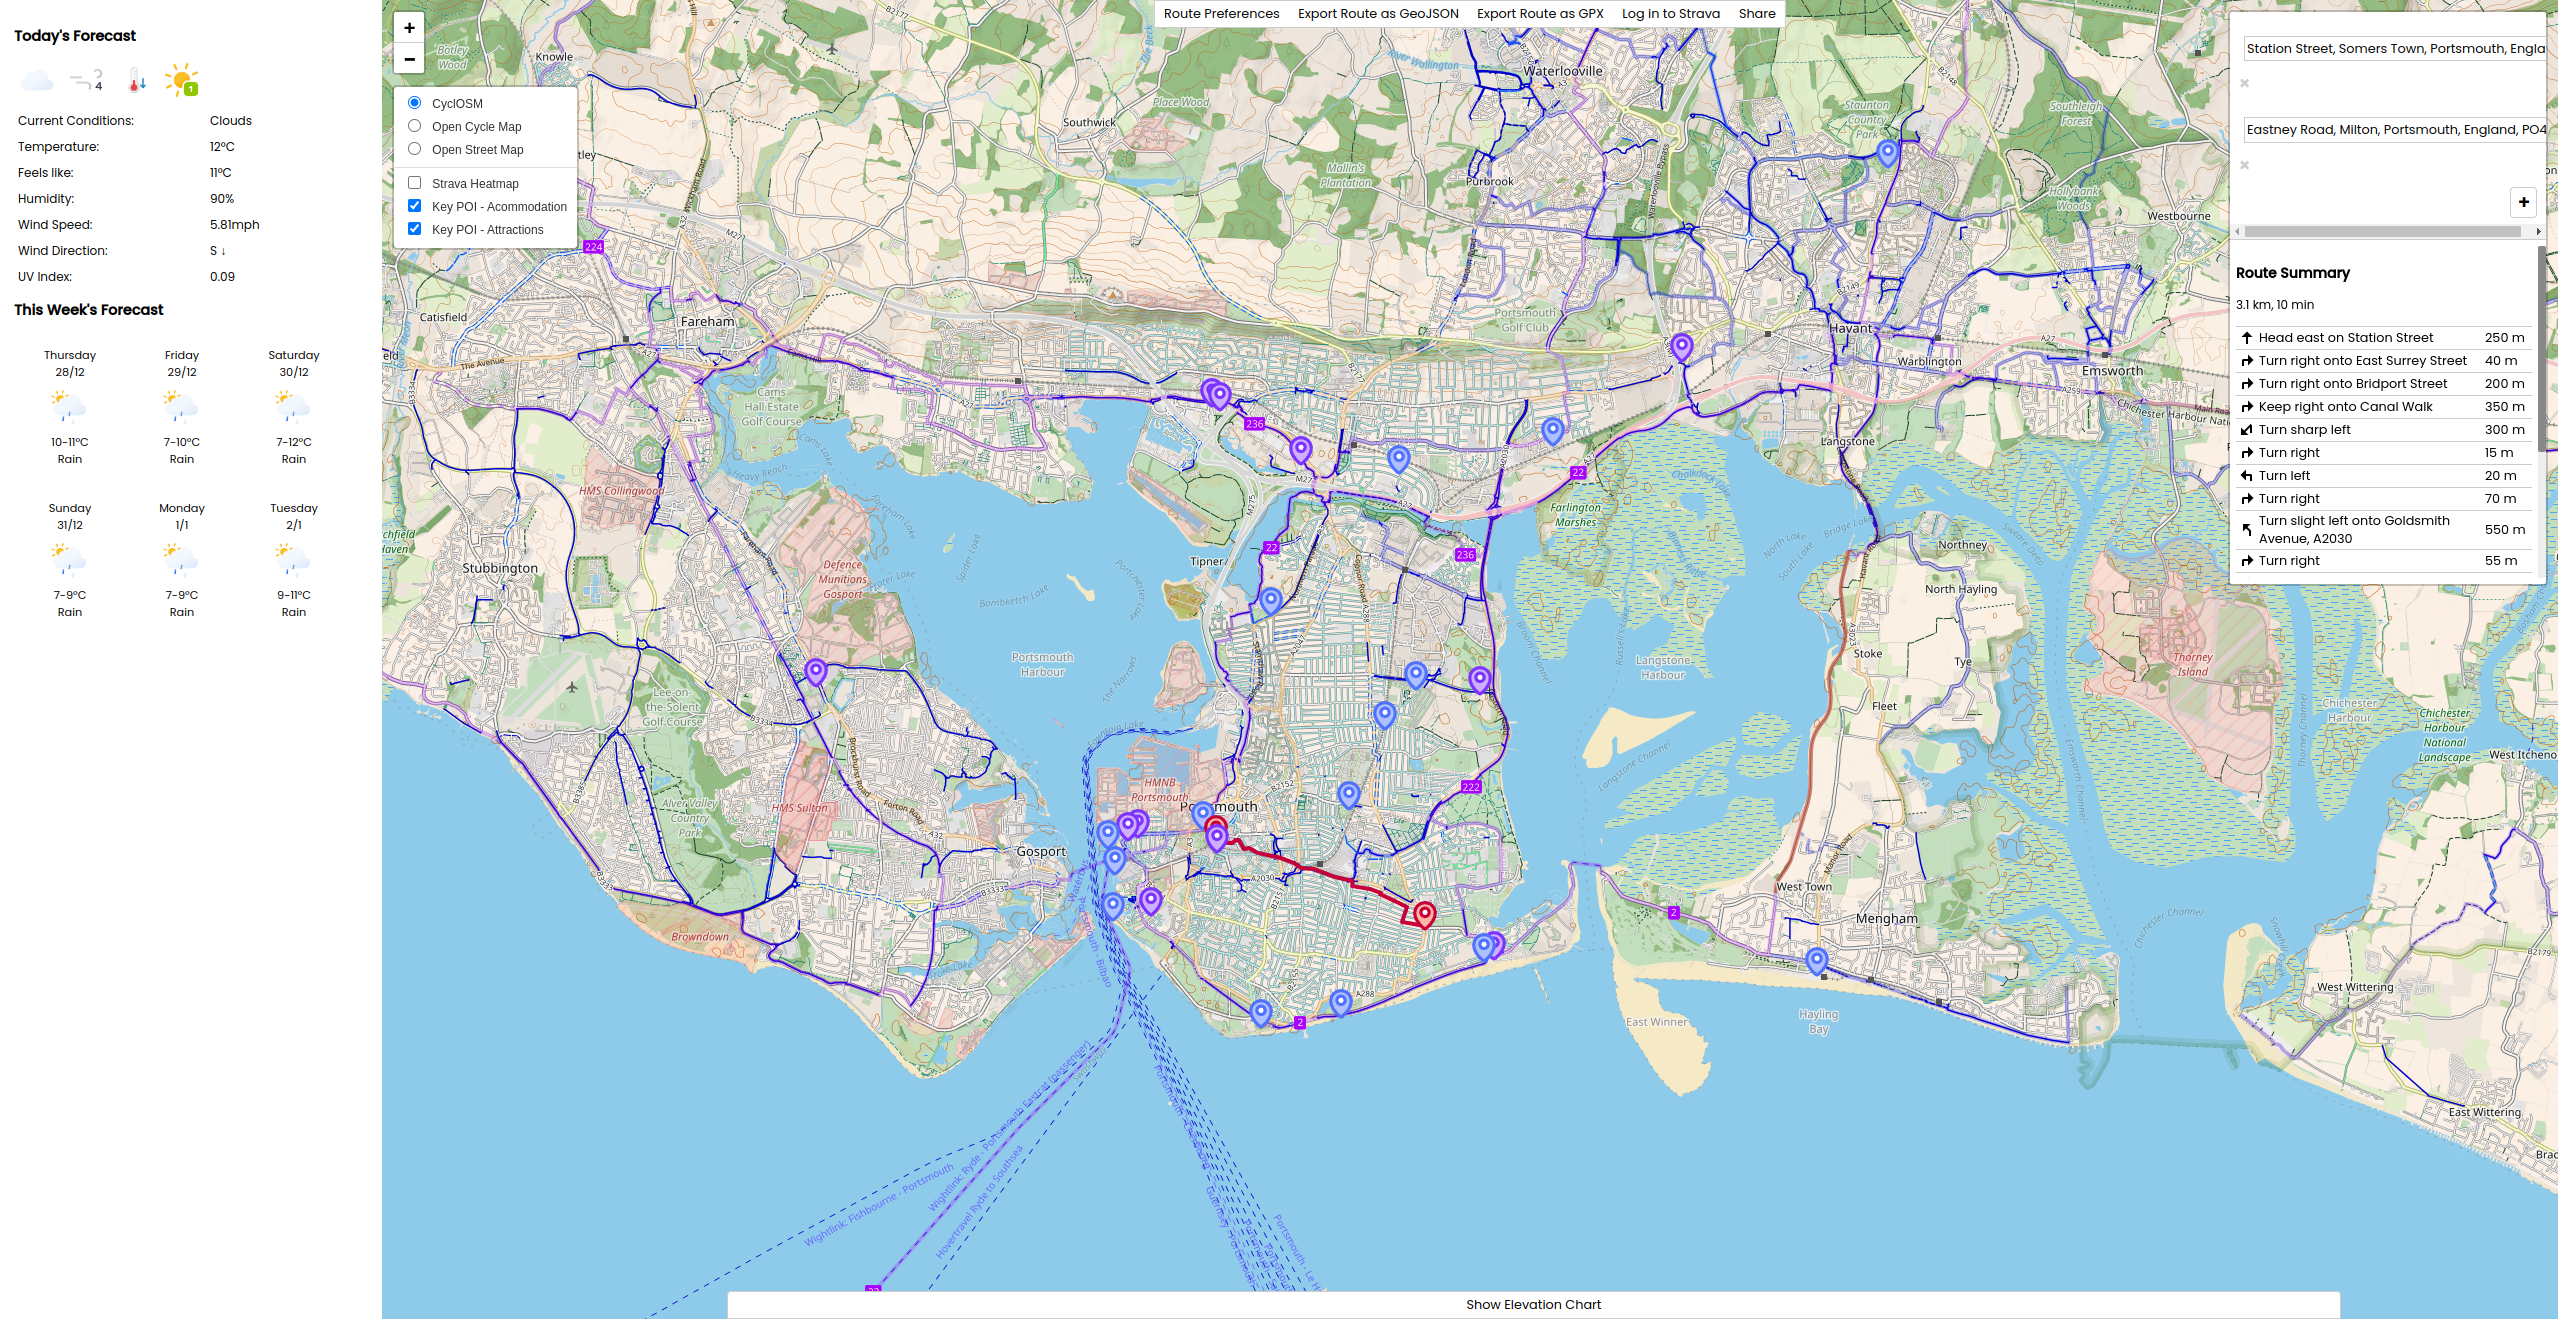
\includegraphics[width=425px]{figures/Progress Images/Iteration-2/SR40-45/SR40 - Attractions and Accommodation KeyPOI.png}
  \caption{Attractions and Accommodation Layers}
  \label{fig:poi-layers}
\end{figure}

\begin{figure}[!ht]
  \centering
  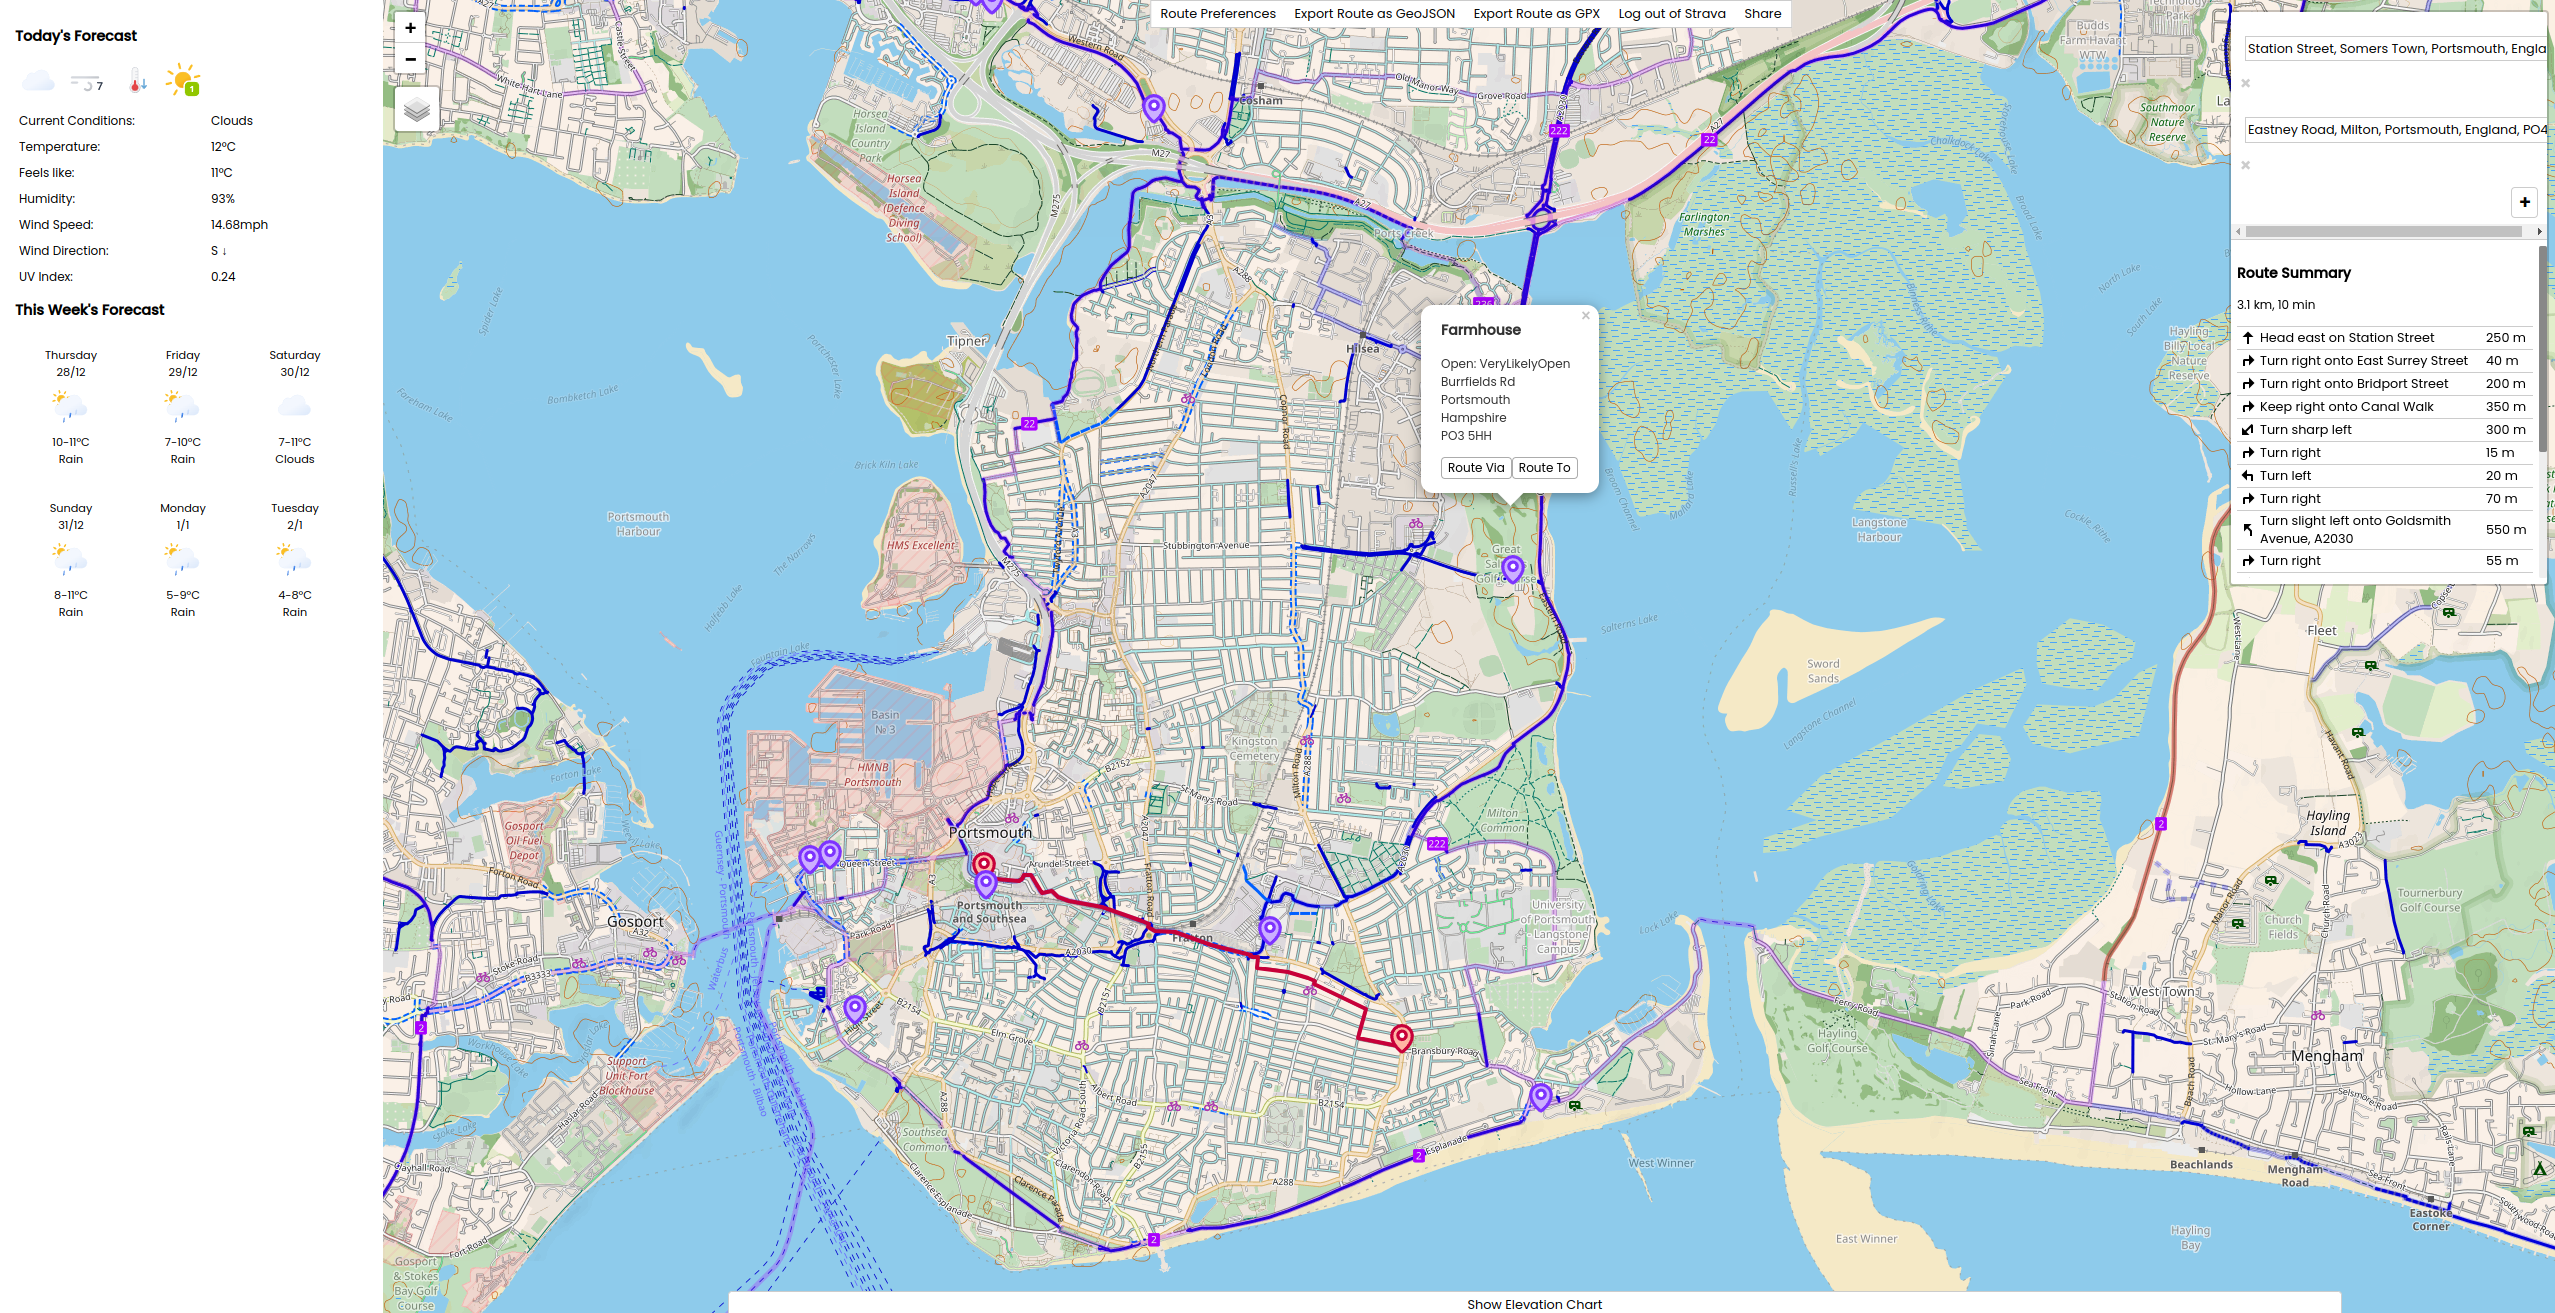
\includegraphics[width=425px]{figures/Progress Images/Iteration-2/SR40-45/SR45 - Route ToVia POI.png}
  \caption{Route To/Via POI}
  \label{fig:poi-route}
\end{figure}

\subsection{Main Challenges}
\label{iteration2:main-challenges}

The main challenges for i2 resided in setting up the SQL queries to handle the hazard data requests as well as oauth authentication with the Strava API.

The INSERT hazard query was the most complex. The PLpgSQL language was used to create a function to handle  this logic as loops were required when inserting multiple PostGIS Point data types (coordinates) for each hazard. A loop was also required to insert the properties for each hazard, where each hazard could have one or more. The function was then called from the API endpoint, passing the json string input directly into the PLpgSQL function as type JSONB.

The Strava API was also challenging as it was required to implement oAuth 2.0 manually to authorise the application to upload activities to the user's account. The Strava API documentation was relatively clear on how to implement this process, however, having not manually implemented oAuth before, without using libraries such as Auth0, it was a steep learning curve. This experience proved great later on however when implementing oAuth 1.0 for use with the Garmin Connect API \see{iteration3:garmin-integration}.

\section{Iteration 3 - Round Trip, Route Import and Garmin Integration}
\label{implementation:iteration3}

\subsection{Round Trip Routing}

\subsection{Route Import}

\subsection{Garmin Connect Integration}
\label{iteration3:garmin-integration}

\subsection{Social Media Sharing}

\subsection{Main Challenges}
\chapter{Testing}
\label{chap:testing}

\section{Unit Testing}
\label{testing:unit}

\subsection{Testing here}
\label{unit:1}

\section{Postman}
\label{testing:postman}

\section{Chrome Developer Tools}
\label{testing:chrome-dev}
\chapter{Evaluation}
\label{chap:evaluation}

This chapter evaluates the project as a whole focusing on the development process, and whether the project meets the requirements set out in \autorefp{chap:requirements}. The chapter will also discuss the limitations of the project and potential future work.

\section{Project Timeline and Management}
\label{evaluation:timeline-management}

During the early stages of the academic year, starting a project was exciting and was progressing well. The problem proved challenging over time, yet rewarding when understanding the fundamentals that build route planning systems. Time management, planning and determining theoretical deadlines for development and report writing were crucial to ensuring steady progression despite the pressing deadlines of other modules. Due to this, the project swiftly began to move ahead of schedule, resulting in the initial Gantt chart \see{fig:initial-gantt} being revised to adjust for the rapid progress \see{fig:final-gantt}.

The first iteration began around November before the designs were complete and the requirements gathering phase had begun. This led to the first iteration being developed blindly, with no clear direction. Therefore, the first iteration merely set up the basic structure of the system, leading to development choices that would later not align with the requirements \see{chap:requirements}. Furthermore, because development began before designs were also complete, the iteration didn't accommodate for the design decisions made after the iteration was complete \see{chap:design}. This led to a significant amount of refactoring in the second iteration, which could have been avoided if the development was started after the designs were complete.

The development methodology also changed after iteration 1 was complete, moving from an incremental to an iterative approach. The incremental approach was not feasible due to the complexity of the project, it proved beneficial to progressively build and improve all aspects of the system in iterations. Allowing for the system to be built in a modular fashion, enabling easier integration of new features and changes.

The final Gantt chart demonstrates the ongoing process of the project, with a dedicated development period catered around the report's progress. The core development periods were between November and December, then January to the start of semester two. Approximately, development consisted of two months, on average twenty to twenty-five hours each week. Breaking up the development in such a way enabled both development and report writing to be progressing simultaneously without one hindering the other.

Overall the project was managed more effectively than originally planned, running ahead of schedule throughout the academic year. The extra time allowed for refinements and improvements without the pressure of an immediate deadline. Constant feedback from the client yielded a more developed understanding of the requirements, the project direction and suggestions for new requirements. The requirements originated as user stories, broken down into smaller, system requirements. Doing so made the use of GitHub projects and issues more effective with the ability to visualise project progress, further aiding an iterative agile development process.

To summarise, the project was managed effectively, except for the early start of iteration 1. The time spent on both development and report writing was well-balanced around other modules and commitments, limiting the chance of burnout. The primary issue was the early stages where development decisions were made without designs and requirements resulting in a knock-on effect in later project stages when integrating more complex features with pre-existing code. It is critical to ensure the project is well planned and development doesn't begin until the requirements and designs are complete to limit the chance of future rework and refactoring.

\begin{figure}[h!]
    \centering
    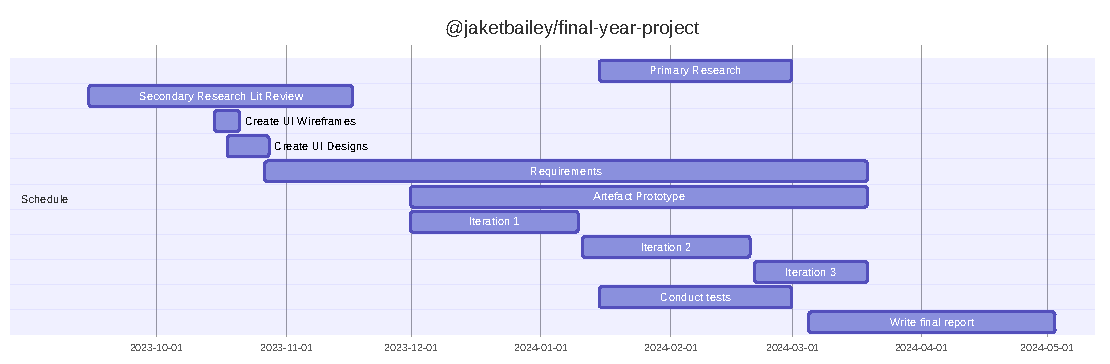
\includegraphics[width=1\linewidth]{figures/Old FYP Gantt - Timeline 1.pdf}
    \caption{Initial Gantt Chart}
    \label{fig:initial-gantt}
\end{figure}

\begin{figure}[h!]
    \centering
    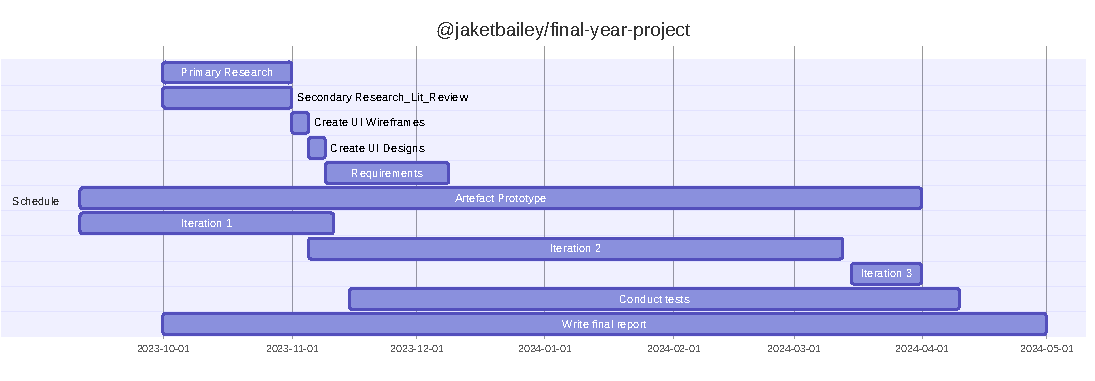
\includegraphics[width=1\linewidth]{figures/Actual FYP Gantt.pdf}
    \caption{Final Gantt Chart}
    \label{fig:final-gantt}
\end{figure}

\clearpage
\section{Evaluating Requirements}
\label{evaluation:requirements}

For this project, assessing its success based solely on the fulfilment of the defined requirements might not provide a comprehensive evaluation. All requirements were established ahead of the three development iterations, with a revision made after primary research was completed \see{fig:research-results}. User stories were created and broken down into smaller system requirements, which were assigned to the development iterations based on priority order via the MoSCoW method \see{chap:requirements}. Further analysis was required to determine if all requirements were met and if they combined to meet all objectives. For all discussion surrounding the project's objectives \see{chap:reflection-and-conclusion}.

Overall, 47 of 51 system requirements were met \see{evaluatedrq}. The four requirements not met were due to the prioritisation of other requirements, the missed requirements were not critical to the system's functionality. They were not met because of the focus on \hyperref[SR:50]{SR50} at the end of development which was a complex but ideal feature to implement. Therefore, some of the initial requirements were not met. Should there have been extra development time, these would be the first to be implemented.

The requirements missed were primarily from 'User Story 05' \see{tab:user-story-05} as these were marked as 'Could' with the MoSCoW method. These focused on integrating weather data into the route planning algorithm. Whilst consideration occurred for extending development and implementation, there was no such weather data API that could serve effectively for this specific purpose. This was due to limited funds and the complexity of the feature.

All requirements met can be evidenced by the work undertaken within the 'Implementation' chapter of this report \see{chap:implementation}. The routing machine provides users with core routing functionality and customisability (\hyperref[tab:user-story-02]{User Story 02}), whilst providing the user with the ability to export and share routes locally or to external services such as Garmin, Strava and Google Drive (\hyperref[tab:user-story-03]{User Story 03}, \hyperref[tab:user-story-04]{User Story 04}) \see{fig:garmin-connect}. Furthermore, the map component enables users to view and manipulate the route (\hyperref[tab:user-story-06]{User Story 06}) \see{fig:route-import}.

Many requirements were reliant on others to be built first, therefore the MoSCoW method was used to determine the prioritisation based on user feedback with consideration of requirements' dependencies on other requirements. This enabled a functional, well-rounded system to be developed in a logical order, with a focus on modularity. Reflections on the requirements and objectives can be found in the conclusion \see{reflection-and-conclusion:outcomes/objectives-met}.

\begingroup
\setlength{\tabcolsep}{10pt} % Default value: 6pt
\renewcommand{\arraystretch}{1.5} % Default value: 1
\begin{table}[!htb]
\caption{Requirements Evaluation}
\label{evaluatedrq}
\small
    \begin{tabularx}{\textwidth}{ p{1cm} p{11cm} p{1cm} }
        \hline
        ID & Description & Met? \\ 
        \hline
        & \textbf{\hyperref[tab:user-story-01]{User Story 01}} \\
        \hyperref[SR:1]{SR1} & The system must provide a route configuration panel. & Y\\
        \hyperref[SR:2]{SR2} & The route configuration page must provide a starting and destination location input field. & Y\\
        \hyperref[SR:3]{SR3} & The route configuration page should suggest accurate geolocations based on the location inputs.  & Y\\
        \hyperref[SR:4]{SR4} & The route configuration page must determine the geolocation based on the user input. & Y\\
        \hyperref[SR:5]{SR5} & The route configuration page must plan the route once two or more locations are input. & Y\\
        \hline
        & \textbf{\hyperref[tab:user-story-02]{User Story 02}}  \\
        \hyperref[SR:6]{SR6} & The system must provide an overlay window to allow the user to update routing preferences. & Y\\
        \hyperref[SR:7]{SR7} & The update preferences overlay must provide options to 'avoid' along the route. & Y\\
        \hyperref[SR:8]{SR8} & The update preferences overlay must provide a 'via' user input field. & Y\\ 
        \hyperref[SR:9]{SR9} & The update preferences overlay must provide a 'leave time' user input field. & Y\\ 
        \hyperref[SR:10]{SR10} & The update preferences overlay must provide a 'arrive time' user input field. & Y\\ 
        \hyperref[SR:11]{SR11} & The update preferences overlay must provide a 'round trip' user input field. & Y\\ 
        \hline
        & \textbf{\hyperref[tab:user-story-03]{User Story 03}}  \\
        \hyperref[SR:12]{SR12} & The system must provide an option to export the planned route. & Y \\
        \hyperref[SR:13]{SR13} & The system must provide an export feature to export the route to the 'GPX' file format. & Y\\
        \hyperref[SR:14]{SR14} & The system must provide an export feature to export the route to the 'GeoJSON' file format. & Y\\ 
        \hyperref[SR:15]{SR15} & The system must provide an export online (to Google Drive, OneDrive and/or other cloud services) & Y\\
        \hline
        & \textbf{\hyperref[tab:user-story-04]{User Story 04}}  \\
        \hyperref[SR:16]{SR16} & The system must provide a share functionality overlay. & Y \\
        \hyperref[SR:17]{SR17} & The share overlay must provide an option to share direct over email. & Y\\
        \hyperref[SR:18]{SR18} & The system must provide an option to share the route direct to Strava. & Y\\ 
        \hline
    \end{tabularx}
\end{table}
\clearpage

\begin{table}[!htb]
    \ContinuedFloat
    \caption{Requirements Evaluation Continued}
    \label{evaluatedrqextended}
    \small
    \begin{tabularx}{\textwidth}{ p{1cm} p{11cm} p{1cm} }
        \hline
        ID & Description & Met? \\ 
        \hline
        & \textbf{\hyperref[tab:user-story-05]{User Story 05}} \\
        \hyperref[SR:19]{SR19} & The system must provide the user with a weather condition overlay. & Y \\
        \hyperref[SR:20]{SR20} & The weather condition overlay must provide the user with the weather for the current day. & Y\\
        \hyperref[SR:21]{SR21} & The weather condition overlay must provide the user with the weather for the next week. & Y\\
        \hyperref[SR:22]{SR22} & The weather condition overlay must provide the user with the option to enable weather conditions in the route planning algorithm. & N\\ 
        \hyperref[SR:23]{SR23} & The weather condition overlay must provide the user with suggestions on the best days to cycle. & N\\
        \hyperref[SR:24]{SR24} & An option to include weather in route planning should be provided, ensuring the user enters the planned day to ride & N\\ 
        \hline
        & \textbf{\hyperref[tab:user-story-06]{User Story 06}}  \\
        \hyperref[SR:25]{SR25} & The system must provide the user with an interactive map to display the planned route. & Y \\
        \hyperref[SR:26]{SR26} & The interactive map must allow the user to zoom into parts of the planned route. & Y\\
        \hyperref[SR:27]{SR27} & The interactive map must allow the user to select parts of the route and receive detailed information about that subsection of the route. & Y\\
        \hyperref[SR:28]{SR28} & The interactive map must allow the user to select and drag the planned route to modify its path. & Y\\ 
        \hyperref[SR:29]{SR29} & The system must display an elevation graph for the planned route beneath the interactive map. & Y\\
        \hyperref[SR:30]{SR30} & The system must allow the user to measure chosen sections of the route & Y\\
        \hyperref[SR:31]{SR31} & The system must provide multiple map layers to give users the greater options when viewing the route & Y\\ 
        \hline
        & \textbf{\hyperref[tab:user-story-07]{User Story 07}}  \\
        \hyperref[SR:32]{SR32} & The system must provide a user input modal to input Hazard and Infrastructure Data. & Y \\
        \hyperref[SR:33]{SR33} & The hazard input modal must provide a Type drop-down menu based on the OSM Hazard Types. & Y\\
        \hyperref[SR:34]{SR34} & The hazard input modal must provide a date entry point to specify the date the hazard was seen. & Y\\
        \hyperref[SR:35]{SR35} & The hazard input modal must provide a submit button to add the hazard to the hazard index. & Y\\
        \hyperref[SR:36]{SR36} & The infrastructure input modal must provide a Type drop-down menu with different types of cycling/road infrastructure & Y\\
        \hyperref[SR:37]{SR37} & The infrastructure input modal must provide a date entry point to specify when the bad infrastructure was found & Y\\
        \hline
    \end{tabularx}
\end{table}
\clearpage

\begin{table}[!htb]
    \ContinuedFloat
    \caption{Requirements Evaluation Continued}
    \label{evaluatedrqextended2}
    \small
    \begin{tabularx}{\textwidth}{ p{1cm} p{11cm} p{1cm} }
        \hline
        ID & Description & Met? \\ 
        \hline
        & \textbf{\hyperref[tab:user-story-07]{User Story 07 Cont.}}  \\
        \hyperref[SR:38]{SR38} & The infrastructure input modal must provide an input box providing the user with the option to supply more detail & Y\\
        \hyperref[SR:39]{SR39} & Both Hazard and Infrastructure data should be displayed on the map, with an option to toggle on/off, and report errors & Y\\
        \hline
        & \textbf{\hyperref[tab:user-story-08]{User Story 08}}  \\
        \hyperref[SR:40]{SR40} & The system must provide a map layer to include key waypoints. & Y \\
        \hyperref[SR:41]{SR41} & The waypoint layer must provide locations of accommodation along the route. & Y\\
        \hyperref[SR:42]{SR42} & The waypoint layer must provide locations of tourist points along the route & Y\\
        \hyperref[SR:43]{SR43} & The waypoint layers must be able to be toggled on and off & Y\\
        \hyperref[SR:44]{SR44} & Each waypoint must be clickable to provide extra detail on each point & Y\\
        \hyperref[SR:45]{SR45} & Each waypoint must have a button to add stop along the route and the route will be re-plotted via the waypoint. & Y\\
        \hline
        & \textbf{\hyperref[tab:user-story-09]{User Story 09}}  \\
        \hyperref[SR:46]{SR46} & The system must provide an option within the route planning modal to select the rider type. & Y\\
        \hyperref[SR:47]{SR47} & The system must provide an option within the route planning modal to select the fitness level of the rider. & N\\
        \hline
        & \textbf{\hyperref[tab:user-story-10]{User Story 10}}  \\
        \hyperref[SR:48]{SR48} & The system must provide an import option for GPX files. & Y\\
        \hyperref[SR:49]{SR49} & The system must provide an import option for GeoJSON files. & Y\\
        \hline
        & \textbf{\hyperref[tab:user-story-11]{User Story 11}} \\
        \hyperref[SR:50]{SR50} & The system must provide an export to Garmin Routes. & Y\\
        \hyperref[SR:51]{SR51} & The system must provide an option to share to different social media platforms. & Y\\
        \hline
    \end{tabularx}
\end{table}
\endgroup

\clearpage
\section{Limitations}
\label{evaluation:limitations}

The first limitation found was with the routing algorithm and library used to integrate with Leaflet (Leaflet Routing Machine (LRM) and OpenRouteService (ORS). The library was not as customisable as initially thought, leading to the need to fork the connecting library between Routing Machine and ORS to enable round-trip routing. LRM requires a minimum of two inputs (A to B), therefore when implementing round-trip, it was not possible to integrate this into the LRM without significant changes to the library. This feature should have proven simple, however, the limitations of LRM required DOM elements in the UI to be hidden to enable the round trip feature, with custom triggers to remove the 2 input minimum. Ideally, LRM would not be used and a custom routing machine would be built from scratch for future versions of the system.

Furthermore, another limitation found when integrating LRM was the inability to import routes. Currently the system imports routes by parsing either a GPX or GeoJSON file, taking the route coordinates and adding them as a 'Waypoint' in LRM. Each 'Waypoint' acts as a 'via' position in the route. Consequently, in long routes, there can be hundreds of 'Waypoints' which are all added as 'via' points in the UI. This caused many issues when querying geolocation for each waypoint whereby the API would block access due to the number of requests. To resolve this, the system will not make geolocation requests when there are six or more waypoints. The drawback to this is that the system will not provide named locations for waypoints when there are six or more waypoints. These issues with LRM further highlight the need to build a custom routing machine.

Compatibility is another limitation where the system is currently only compatible with desktop devices, having little responsiveness to support mobile. This is because the focus was on desktop-based route planning rather than mobile, however, in future iterations, mobile support will be considered \see{design:assumptions/decisions}. Minimising the amount of overlays on the UI will also be a core focus to improve the user experience, to integrate the overlays into the core UI elements.

A final limitation is the lack of a cloud-based server to store user data and routes. This was a feature that was considered, however, due to the complexity and time constraints, it was not feasible to implement. This would have allowed users to save routes and access them from different devices, as well as share routes with other users. These routes would also be implemented into the social sharing functionality. Direct links to routes would be generated and shared, with the ability to view shared routes natively in the system.

\section{Future Work}
\label{evaluation:future}

The four outstanding requirements that were not met will be migrated into iteration 4. The main focus will be integrating weather data within route planning. The following limitations will also be addressed:
\begin{itemize}
    \item Rewriting the routing machine to increase modularity, include round trip and increase code efficiency.
    \item Improving route import, including support for Garmin, Strava and other services.
    \item Mobile support and minimise the number of floating overlays and integrate into core UI elements.
    \item Implementing a cloud-based server to store user data and routes.
\end{itemize}
Addressing the limitations of the project will be the primary focus, however, the following desired improvements will be implemented:
\begin{itemize}
    \item Implementing a system to allow users to save routes and access them from different devices.
    \item Implementing a system to allow sharing of routes with other users.
    \item Implementing native avoid areas in the route planning algorithm.
\end{itemize}
\chapter{Reflection and Conclusion}
\label{chap:reflectionandconclusion}

%%%%%%%%%%%%%% REFERENCES SECTION
\newpage
\phantomsection
\addcontentsline{toc}{chapter}{References}
% In order to try and get a consistent format I copy and paste the INSPIRE bibtex code into my bibtex file.
\printbibliography

%%%%%%%%%%%% Include your appendices here

\appendix
\chapter{Current Solutions}
\begin{figure}[!ht]
    \centering
    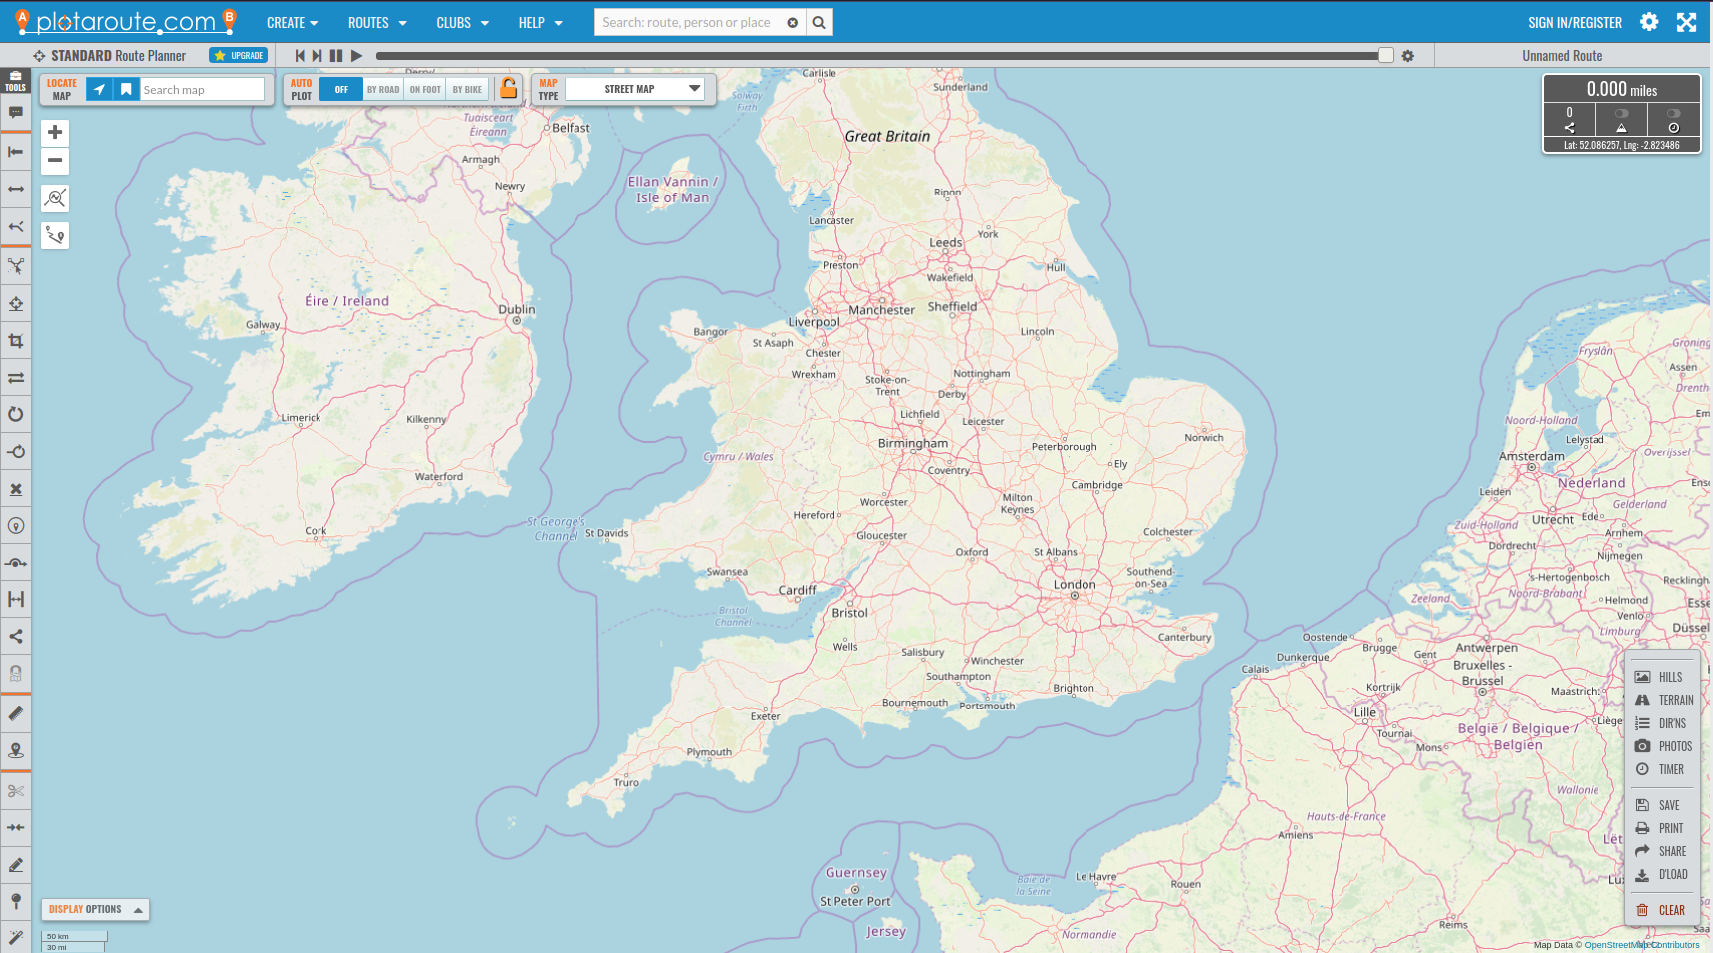
\includegraphics[width=1\linewidth]{figures/plotarouteui.png}
    \caption{Plotaroute.com UI}
    \label{fig:plotarouteui}
\end{figure}

\begin{figure}[!ht]
    \centering
    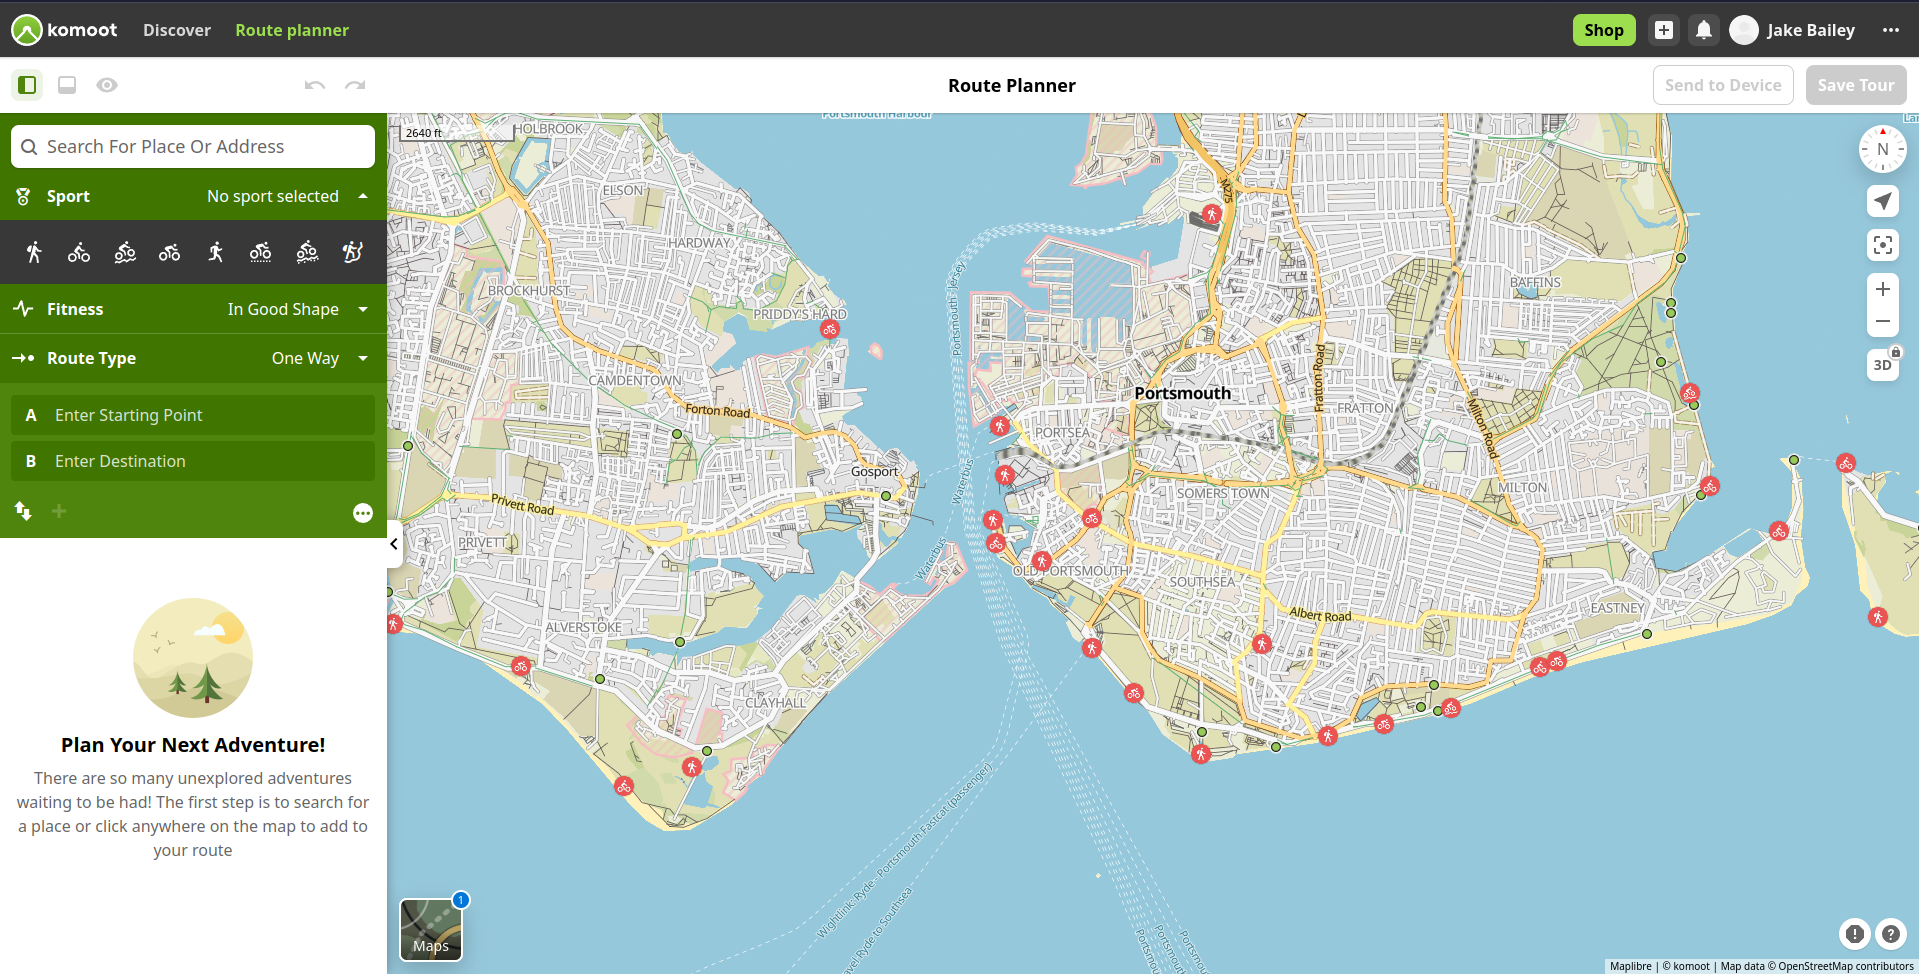
\includegraphics[width=1\linewidth]{figures/komootui.png}
    \caption{Komoot UI}
    \label{fig:komootui}
\end{figure}

\begin{figure}[!ht]
    \centering
    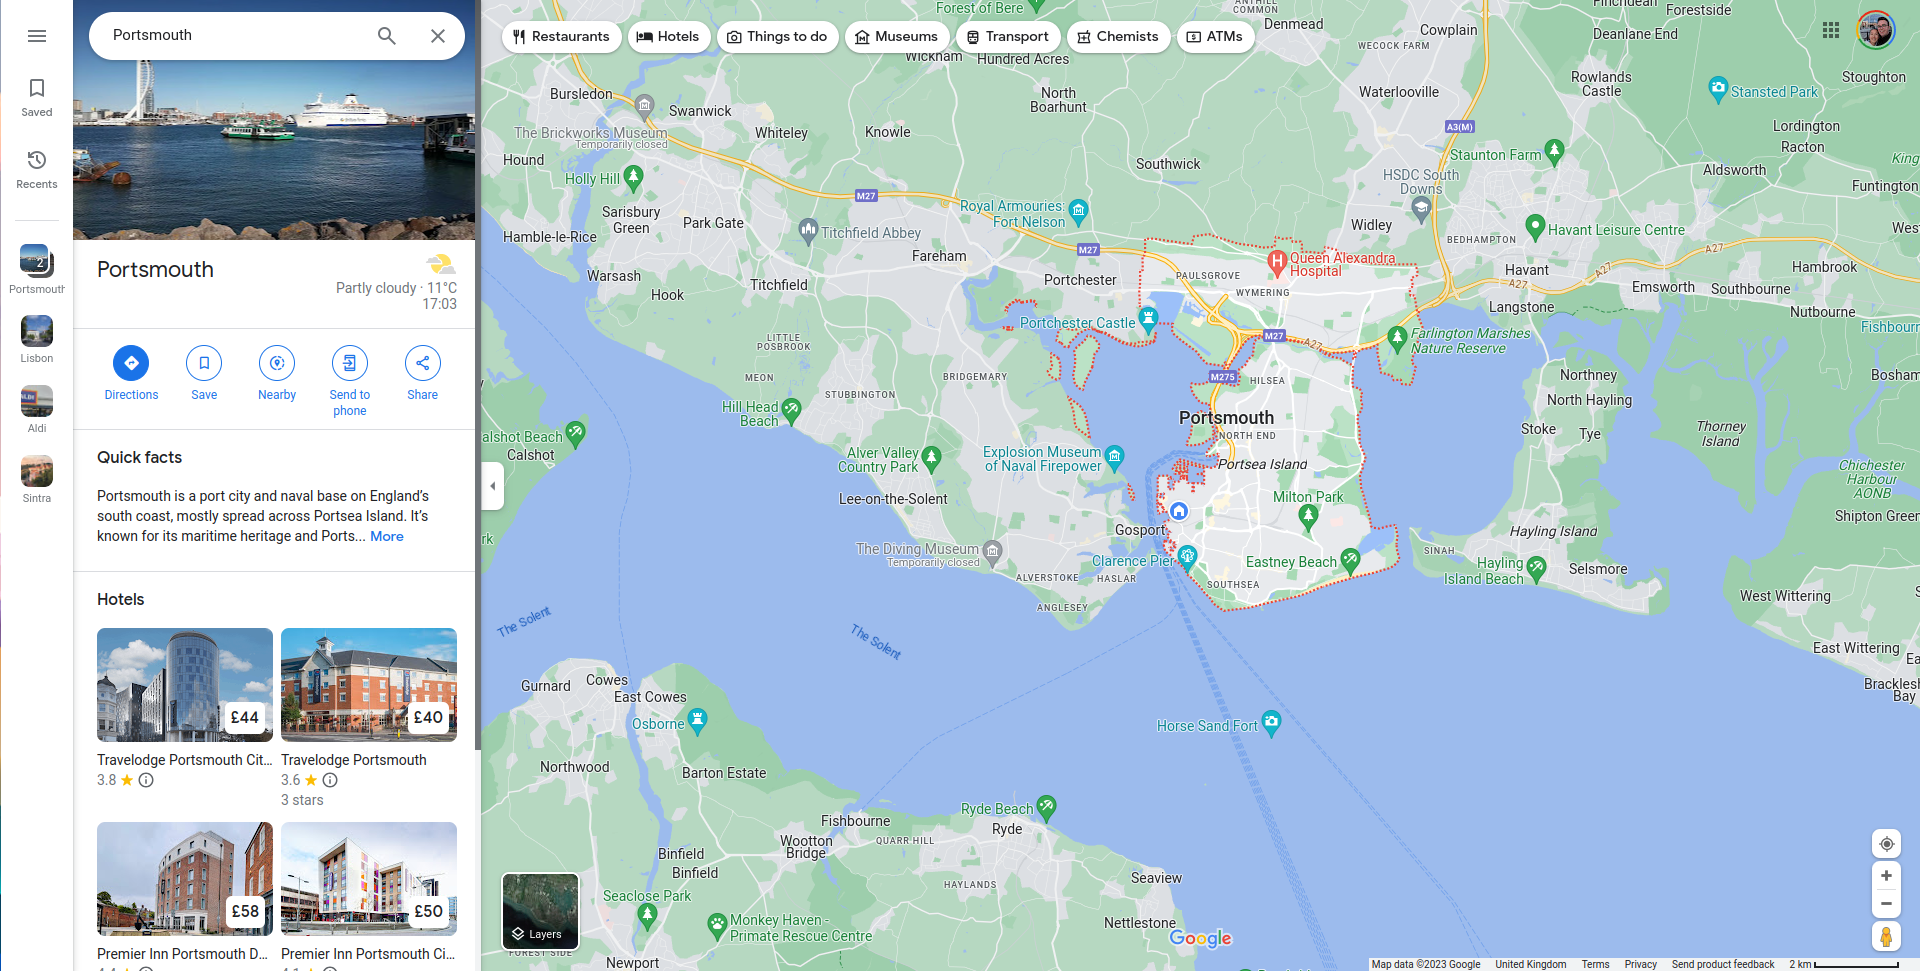
\includegraphics[width=1\linewidth]{figures/gmapsui.png}
    \caption{Google Maps UI}
    \label{fig:gmapsui}
\end{figure}


\chapter{Initial User Requirements}
\begin{table}[!h]
\caption{User Story 01}
\label{tab:user-story-01}
\begin{tabular}{ p{8cm} p{1cm}  p{1cm} }
\hline
\multicolumn{3}{p{13cm}}{As a user, I want a page that allows me to configure my starting and destination location to plan a route.}\\ 
\hline
Acceptance Criteria / System Requirements & Priority & ID\\
\hline
The system must provide a route configuration page. & Must & SR1\\
The route configuration page must provide a starting location input field. & Must & SR2\\
The route configuration page must provide a destination location input field. & Must & SR3\\ 
The route configuration page should suggest locations based on the user input fields. & Should & SR4\\ 
The route configuration page must find the location position based on the user input. & Must & SR5\\ 
The route configuration page must verify both locations are correct before the user can continue. & Must & SR6\\ 
The route configuration page must provide a ‘Plan’ button to initiate the route planning algorithm. & Must & SR7\\ 
\hline
\end{tabular}
\end{table}

\begin{table}[!htb]
\caption{User Story 02}
\label{tab:user-story-02}
\begin{tabular}{ p{8cm} p{1cm}  p{1cm} }
\hline
\multicolumn{3}{p{13cm}}{As a user, I want to change preferences to allow me to customise the route further, including avoiding certain road types and road altitudes.}\\ 
\hline
Acceptance Criteria / System Requirements & Priority & ID\\
\hline
The system must provide an overlay window to allow the user to update routing preferences. & Must & SR8 \\
The update preferences overlay must provide an 'avoid' user input field. & Must & SR9\\
The update preferences overlay must provide a 'via' user input field. & Should & SR10\\ 
The update preferences overlay must provide a 'leave time' user input field. & Should & SR11\\ 
The update preferences overlay must provide a 'arrive time' user input field. & Should & SR12\\ 
The update preferences overlay must provide a 'round trip' user input field. & Could & SR13\\ 
\hline
\end{tabular}
\end{table}

\begin{table}[!htb]
\caption{User Story 03}
\label{tab:user-story-03}
\begin{tabular}{ p{8cm} p{1cm}  p{1cm} }
\hline
\multicolumn{3}{p{13cm}}{As a user, I want to be able to export the planned route for use on my mobile phone or GPS device.}\\ 
\hline
Acceptance Criteria / System Requirements & Priority & ID\\
\hline
The system must provide an option to export the planned route. & Must & SR14 \\
The system must provide an export feature to export the route to the 'GPX' file format. & Must & SR15\\
The system must provide an export feature to export the route to the 'GeoJSON' file format. & Should & SR16\\ 
The system must provide an export feature to export the route direct to Strava. & Could & SR17\\ 
\hline
\end{tabular}
\end{table}

\begin{table}[!htb]
\caption{User Story 04}
\label{tab:user-story-04}
\begin{tabular}{ p{8cm} p{1cm}  p{1cm} }
\hline
\multicolumn{3}{p{13cm}}{As a user, I want to share my route with other people.}\\ 
\hline
Acceptance Criteria / System Requirements & Priority & ID\\
\hline
The system must provide a share functionality overlay. & Should & SR18 \\
The share overlay must provide the user with the option to share direct over email. & Should & SR19\\
The share overlay must provide the user with the option to share direct over Google Drive. & Could & SR20\\ 
The share overlay must provide the user with the option to share direct over OneDrive. & Could & SR21\\ 
The share overlay must provide the user with the option to share direct over Dropbox. & Could & SR22\\ 
\hline
\end{tabular}
\end{table}

\begin{table}[!htb]
\caption{User Story 05}
\label{tab:user-story-05}
\begin{tabular}{ p{8cm} p{1cm}  p{1cm} }
\hline
\multicolumn{3}{p{13cm}}{As a user, I want to be provided with route suggestions based on predicted weather conditions over the week.}\\ 
\hline
Acceptance Criteria / System Requirements & Priority & ID\\
\hline
The system must provide the user with a weather condition overlay. & Must & SR23 \\
The weather condition overlay must provide the user with the weather for the current day. & Must & SR24\\
The weather condition overlay must provide the user with the weather for the next week. & Should & SR25\\
The weather condition overlay must provide the user with the option to enable weather conditions in the route planning algorithm. & Could & SR26\\ 
The weather condition overlay must provide the user with suggestions on the best days to cycle. & Could & SR27\\ 
\hline
\end{tabular}
\end{table}

\begin{table}[!htb]
\caption{User Story 06}
\label{tab:user-story-06}
\begin{tabular}{ p{8cm} p{1cm}  p{1cm} }
\hline
\multicolumn{3}{p{13cm}}{As a user, I want to view the route in detail and get information about parts of the route.}\\ 
\hline
Acceptance Criteria / System Requirements & Priority & ID\\
\hline
The system must provide the user with an interactive map to display the planned route. & Must & SR28 \\
The interactive map must allow the user to zoom into parts of the planned route. & Must & SR29\\
The interactive map must allow the user to select parts of the route and receive detailed information about that subsection of the route. & Should & SR30\\
The interactive map must allow the user to select and drag the planned route to modify its path. & Should & SR31\\ 
The system must display an altitude graph for the planned route beneath the interactive map. & Should & SR32\\ 
\hline
\end{tabular}
\end{table}

\begin{table}[!htb]
\caption{User Story 07}
\label{tab:user-story-07}
\begin{tabular}{ p{8cm} p{1cm}  p{1cm} }
\hline
\multicolumn{3}{p{13cm}}{As a user, I want to input hazards from routes I have cycled so the next route planned would attempt to avoid that area.}\\ 
\hline
Acceptance Criteria / System Requirements & Priority & ID\\
\hline
The system must provide a user input modal to input Hazard Data. & Must & SR33 \\
The user input modal must provide a Type drop-down menu based on the OSM Hazard Types. & Must & SR34\\
The user input modal must provide a date entry point to specify the date the hazard was seen. & Should & SR35\\
The user input modal must provide a submit button to add the hazard to the hazard index. & Must & SR35\\ 
\hline
\end{tabular}
\end{table}

% \chapter{Ethics Certificate}
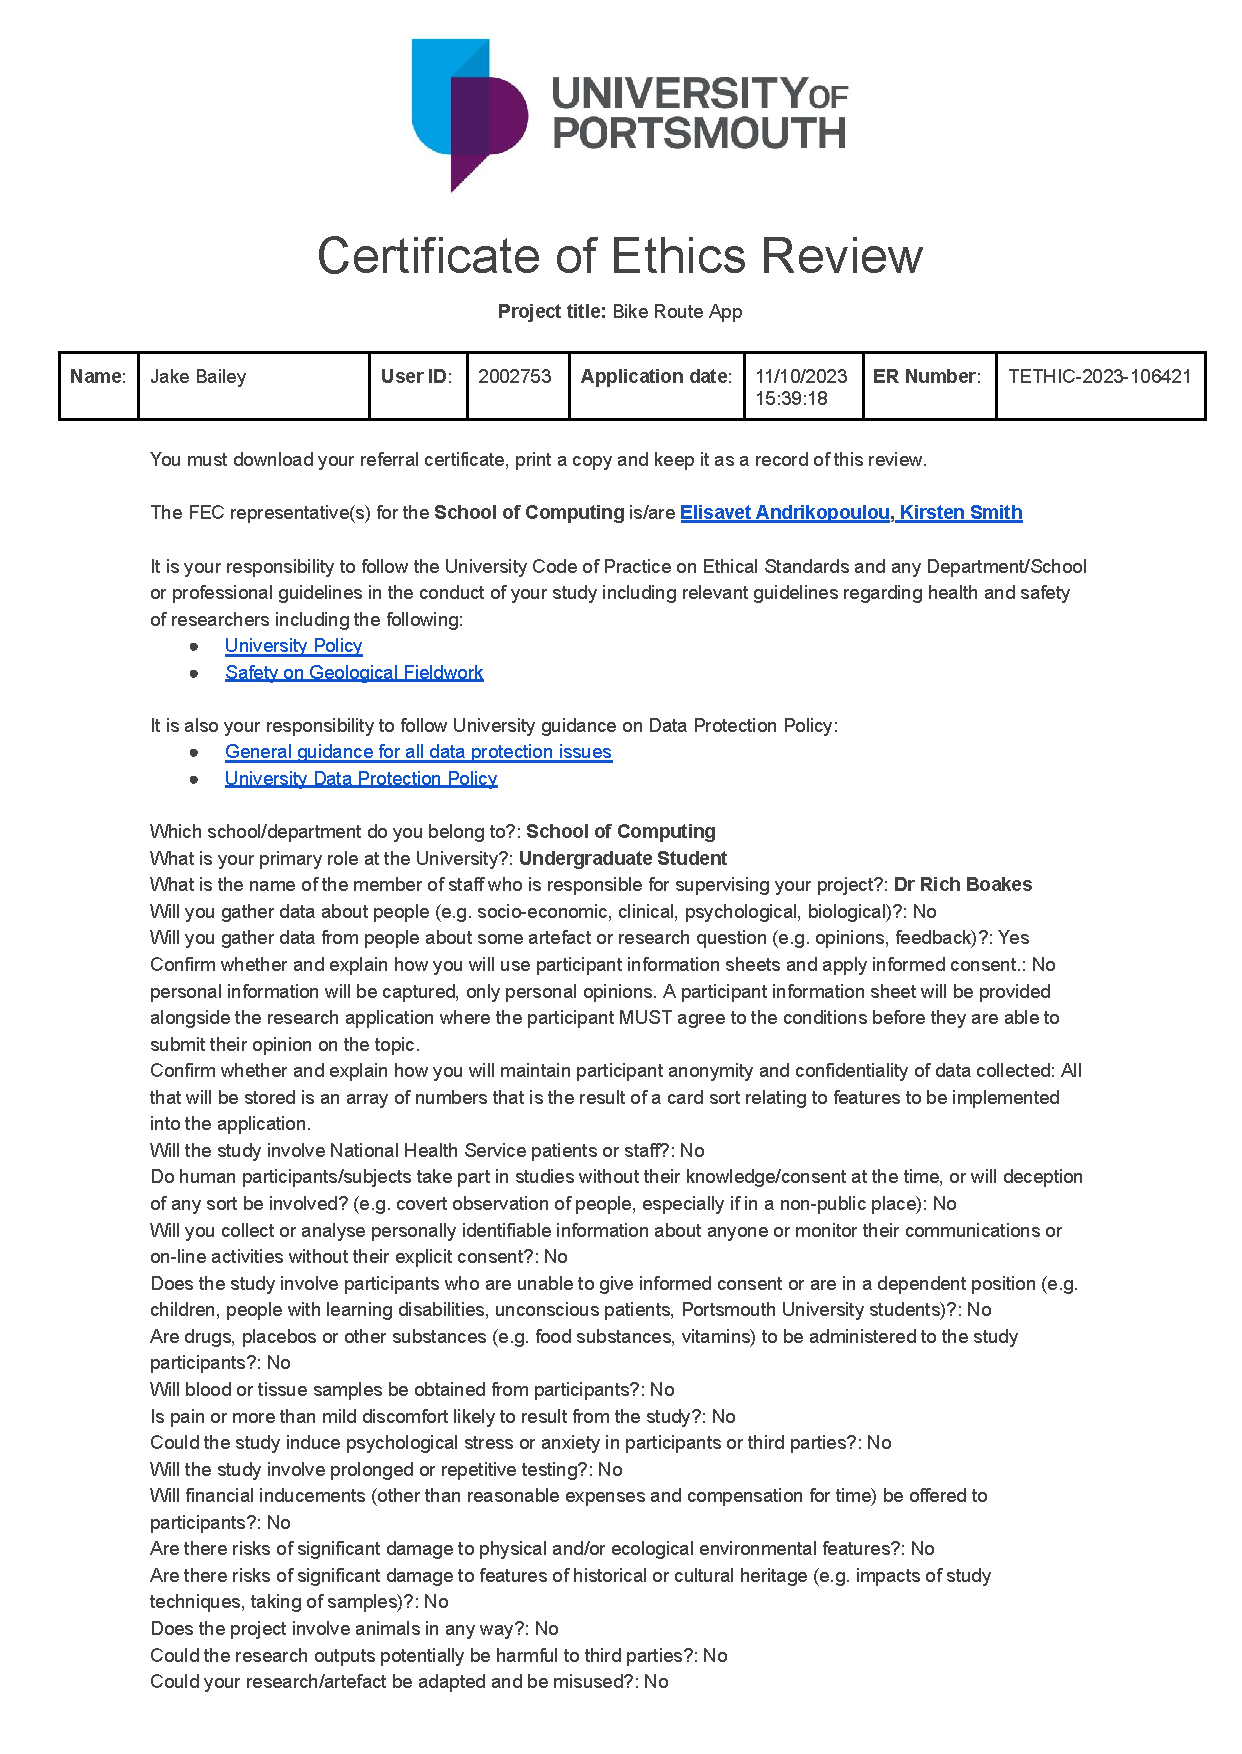
\includepdf[pages=-]{figures/ethics_certificate.pdf}

% \chapter{Increment 2 Screenshots}

\begin{figure}[!ht]
    \centering
    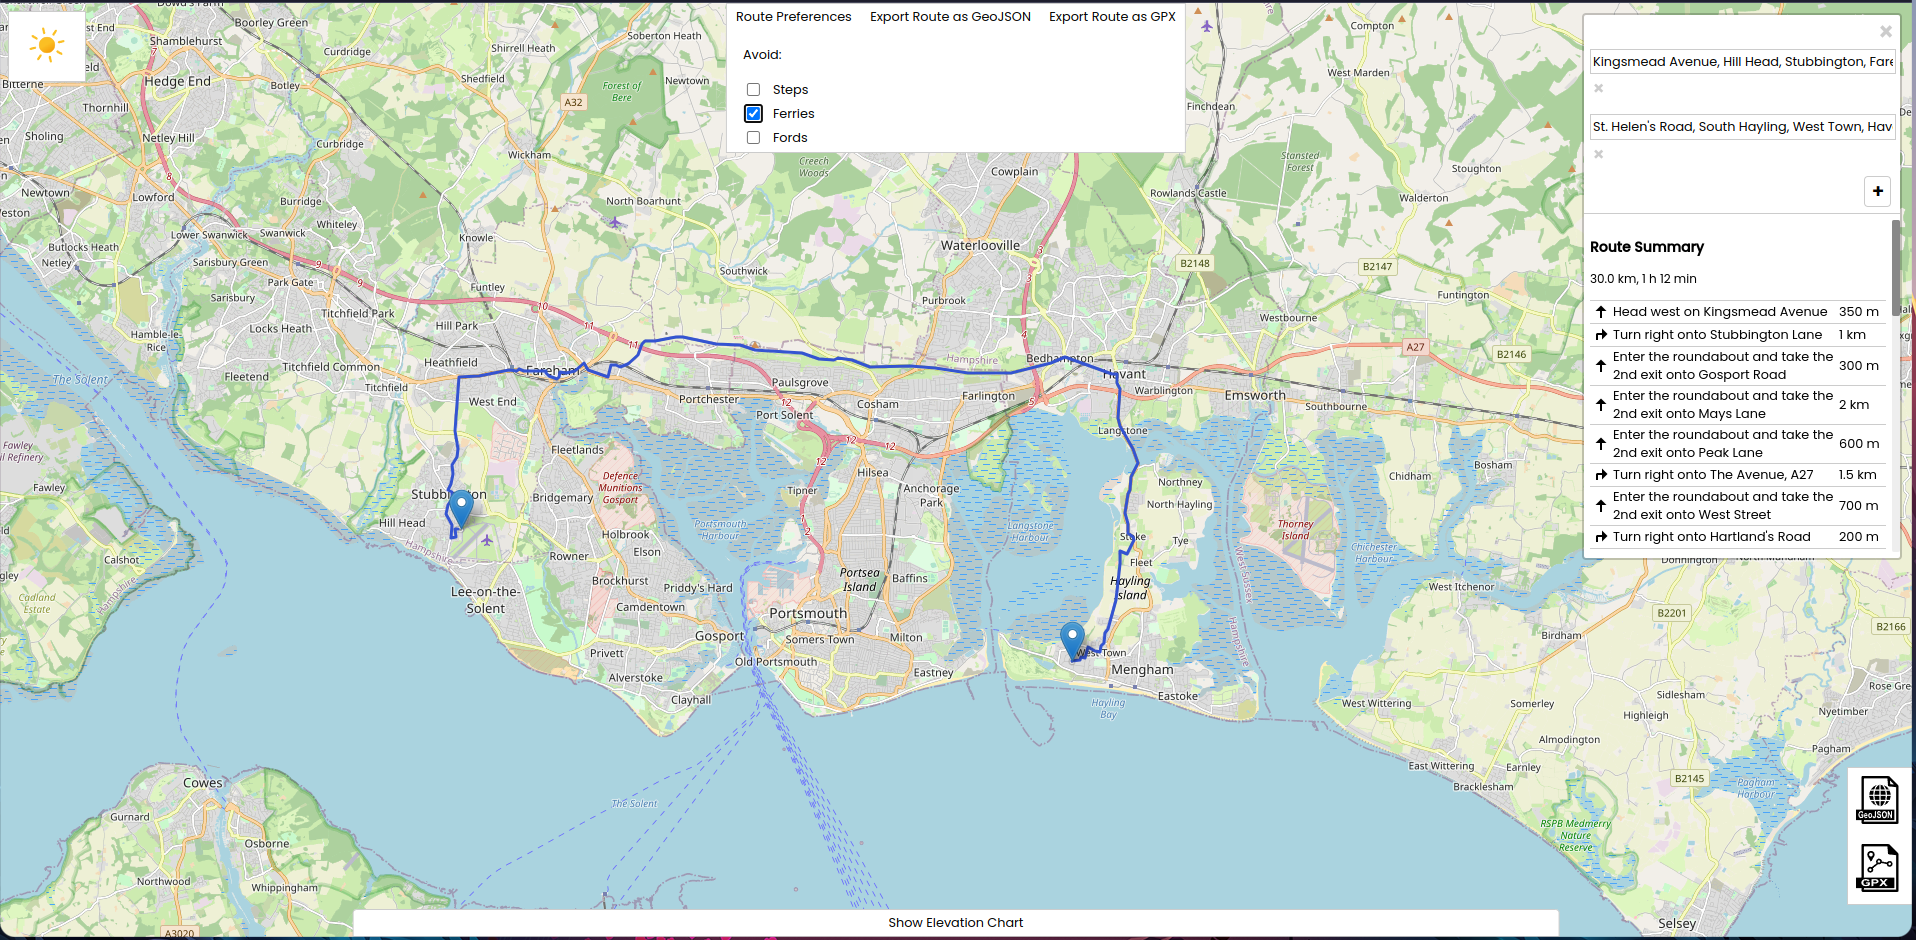
\includegraphics[width=425px]{figures/Progress Images/Iteration-1/SR7/SR9 Top Panel added and Avoid functionality implemented Avoid Ferries Example.png}
    \caption{Top Panel Added}
    % \label{fig:Top-Panel-added}
\end{figure}

\begin{figure}[!ht]
    \centering
    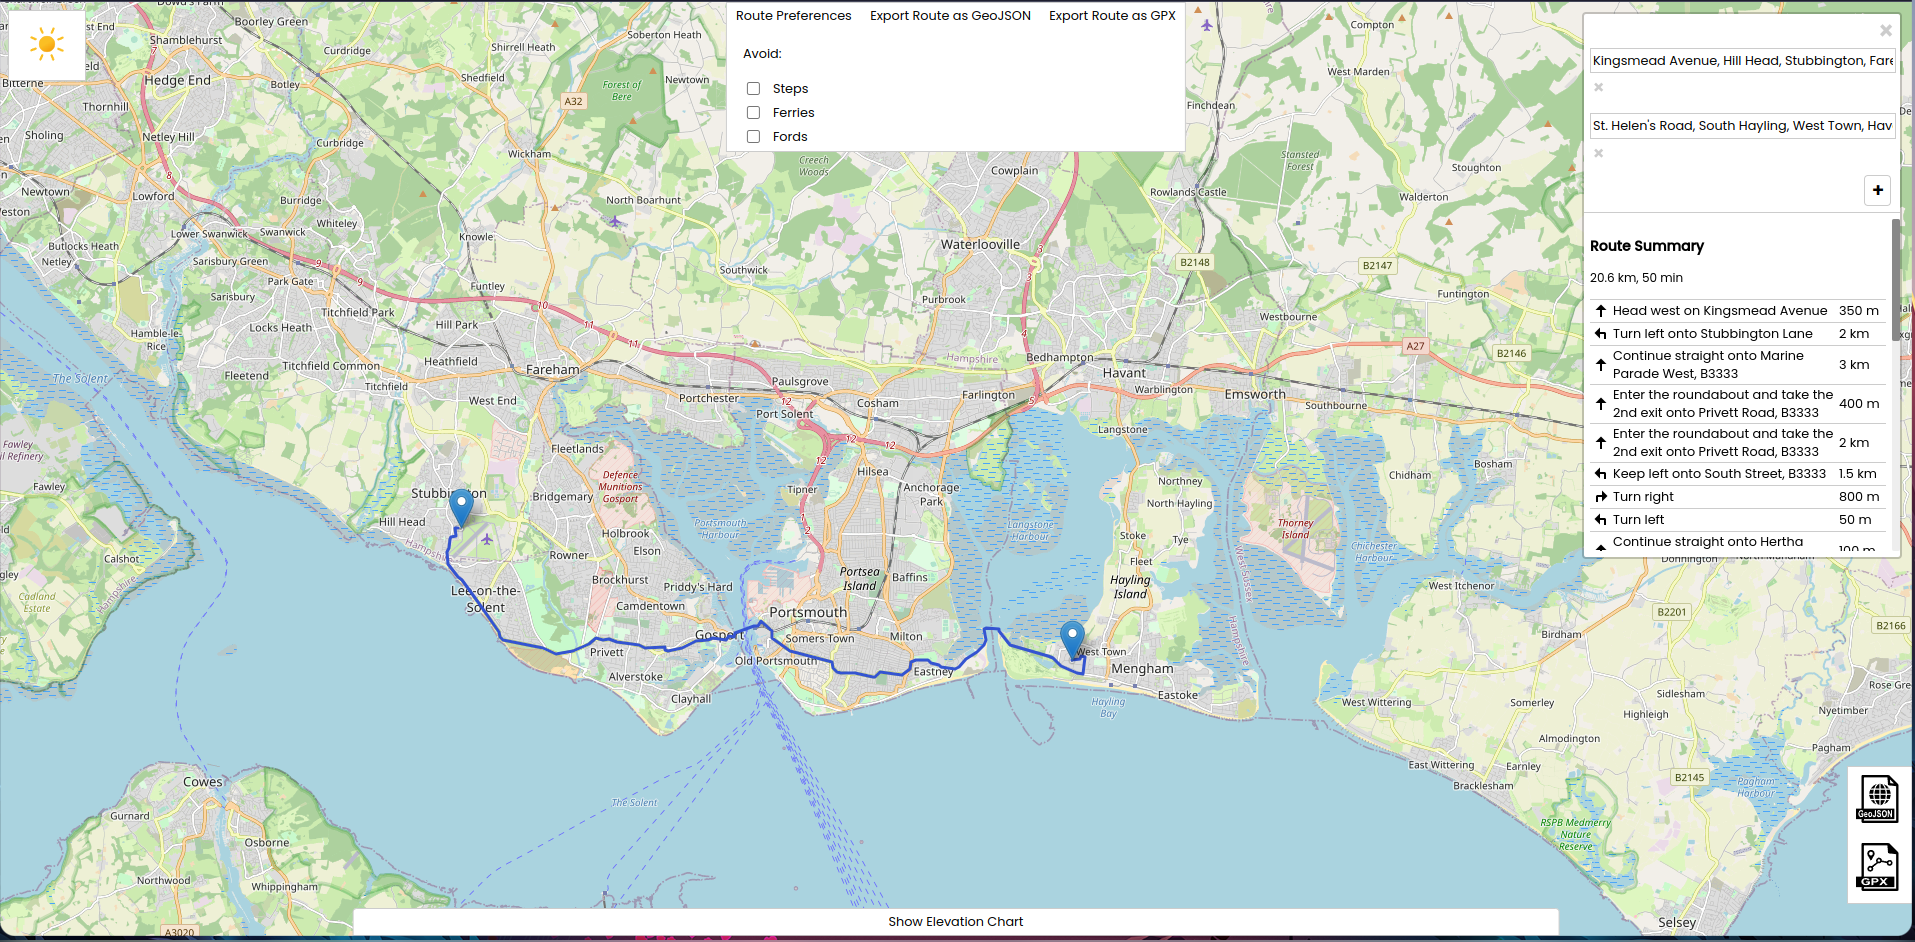
\includegraphics[width=425px]{figures/Progress Images/Iteration-1/SR7/SR9 Top Panel added and Avoid functionality implemented.png}
    \caption{Top Panel Added 2}
    % \label{fig:Top-Panel-added2}
\end{figure}

\begin{figure}[!ht]
    \centering
    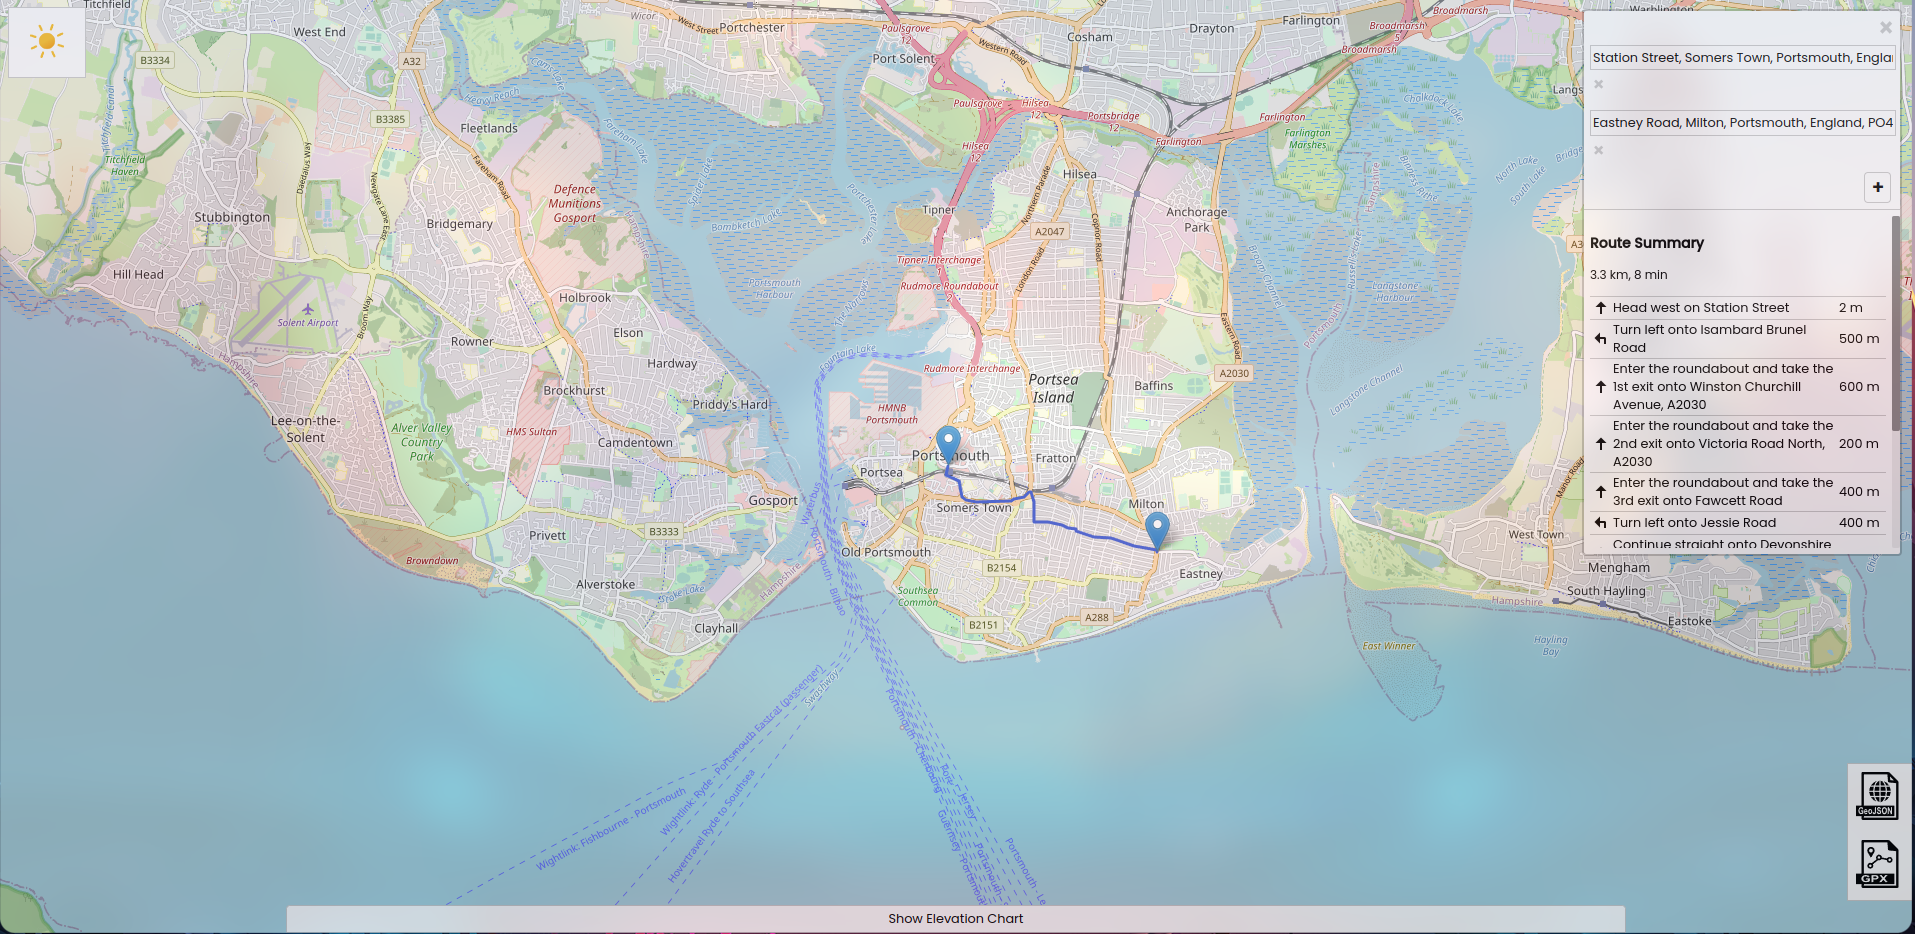
\includegraphics[width=425px]{figures/Progress Images/Iteration-1/SR12/SR13 GPX Icon Added (bottom right).png}
    \caption{GPX Icon Added}
    % \label{fig:gpx-icon-added}
\end{figure}

\begin{figure}[!ht]
    \centering
    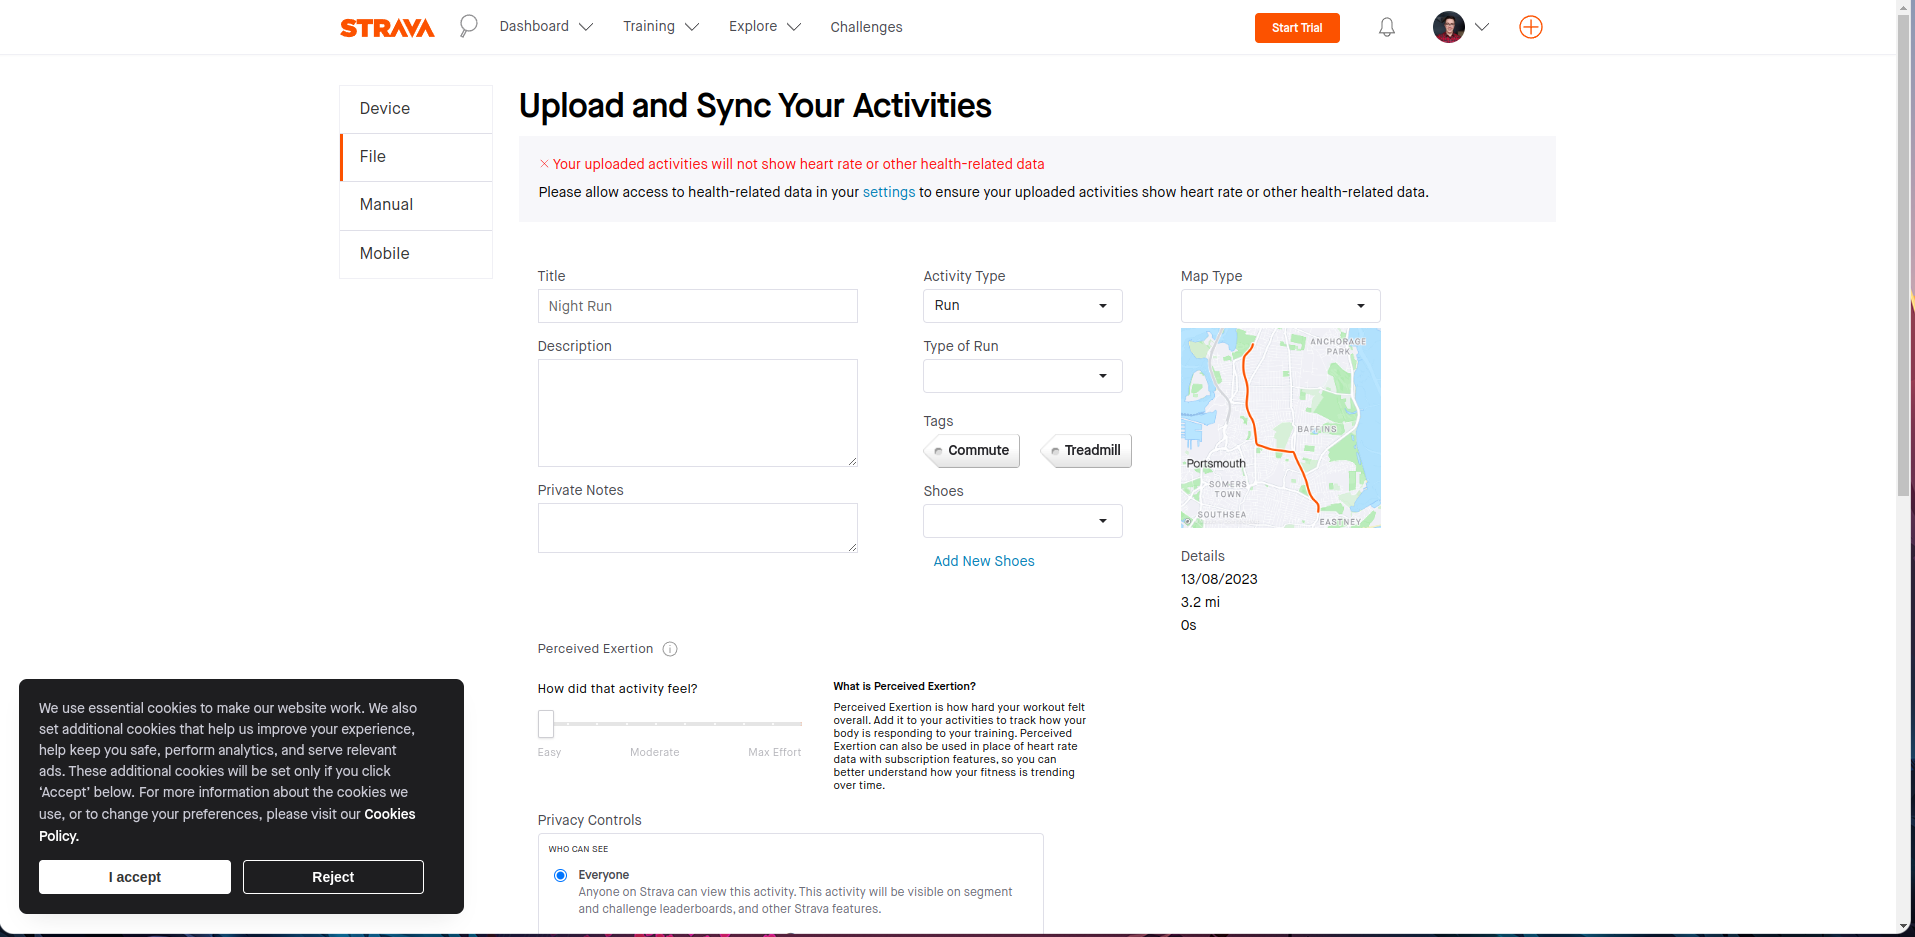
\includegraphics[width=425px]{figures/Progress Images/Iteration-1/SR12/SR13 GPX Successful upload Strava (manual).png}
    \caption{Manual Strava GPX Upload Test}
    % \label{fig:manual-strava-gpx}
\end{figure}

\begin{figure}[!ht]
    \centering
    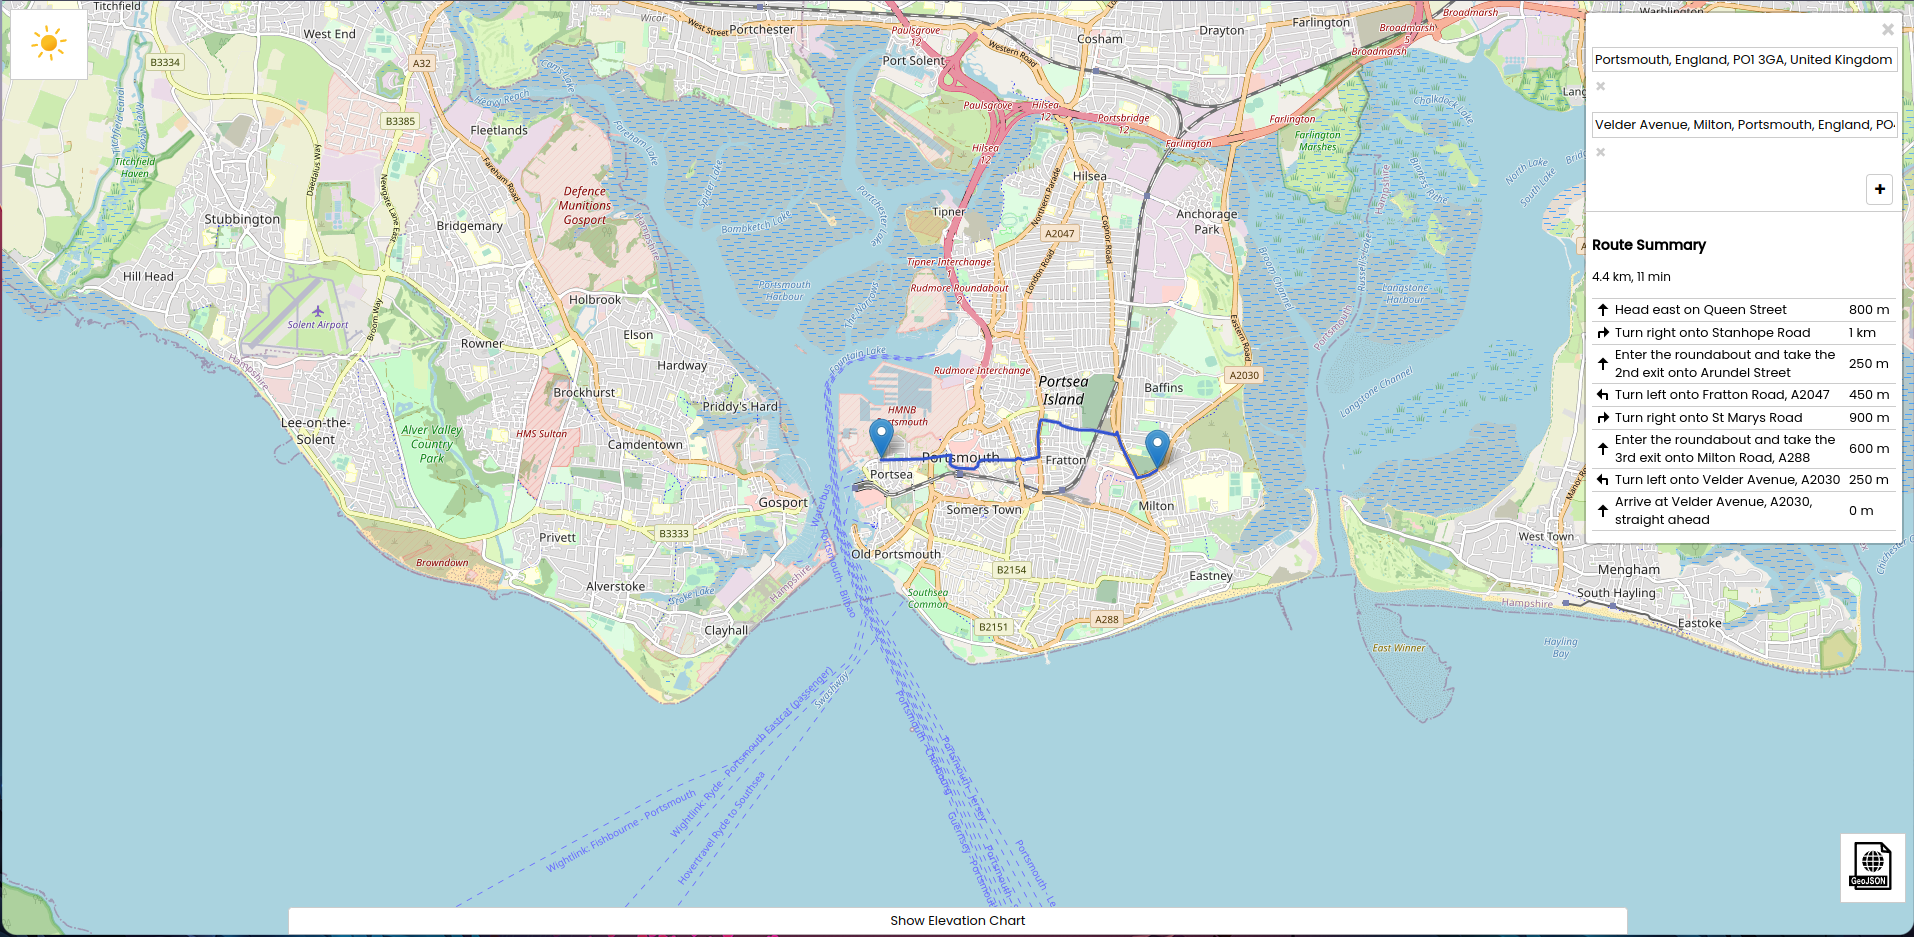
\includegraphics[width=425px]{figures/Progress Images/Iteration-1/SR12/SR14 GeoJSON Export.png}
    \caption{GeoJSON Export}
    % \label{fig:geojson-export}
\end{figure}

\begin{figure}[!ht]
    \centering
    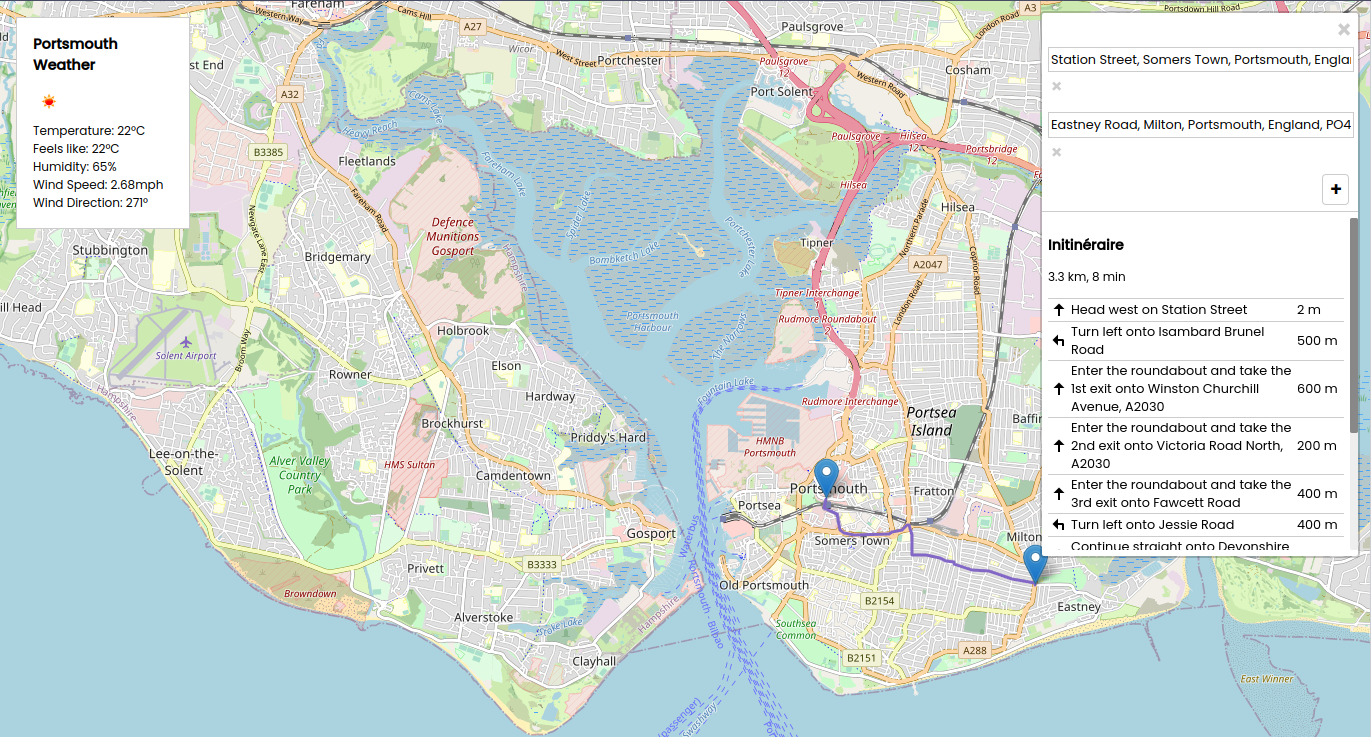
\includegraphics[width=425px]{figures/Progress Images/Iteration-1/SR19/Basic Weather Panel.png}
    \caption{Old Weather Panel}
    % \label{fig:basic-weather-panel2}
\end{figure}

\begin{figure}[!ht]
    \centering
    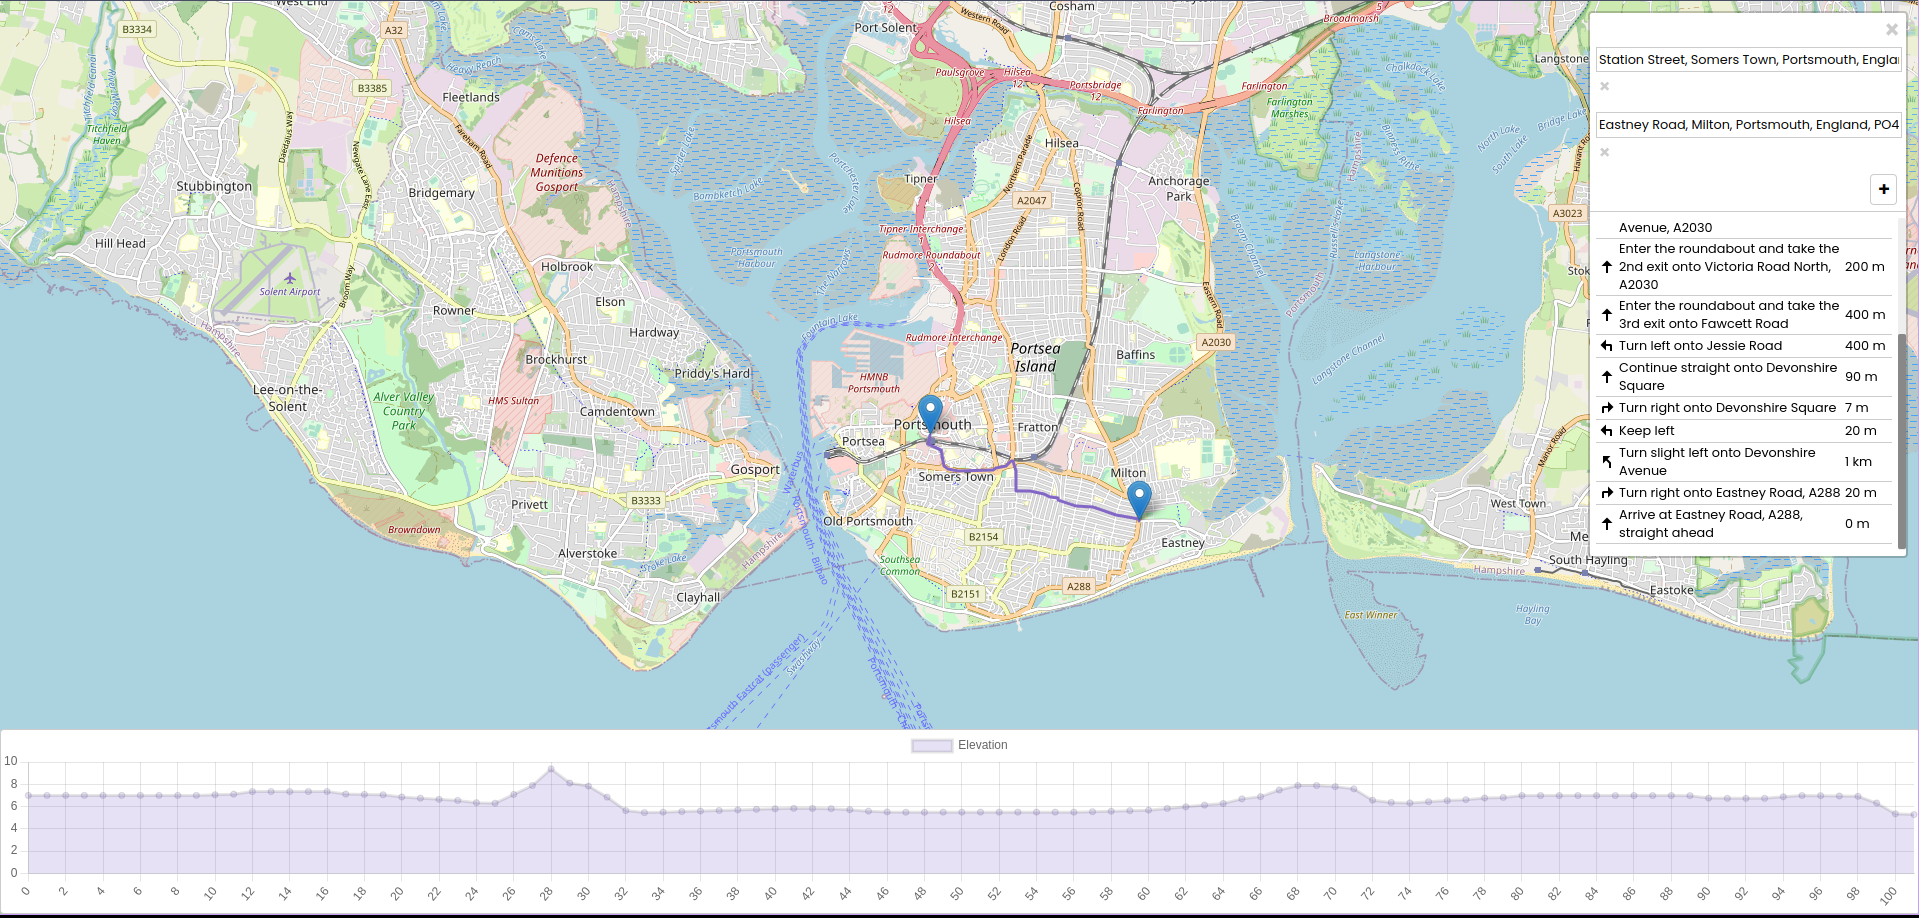
\includegraphics[width=425px]{figures/Progress Images/Iteration-1/SR28/Basic Elevation Plot.png}
    \caption{Basic Elevation Plot}
    % \label{fig:basic-elev-plot}
\end{figure}

\begin{figure}[!ht]
    \centering
    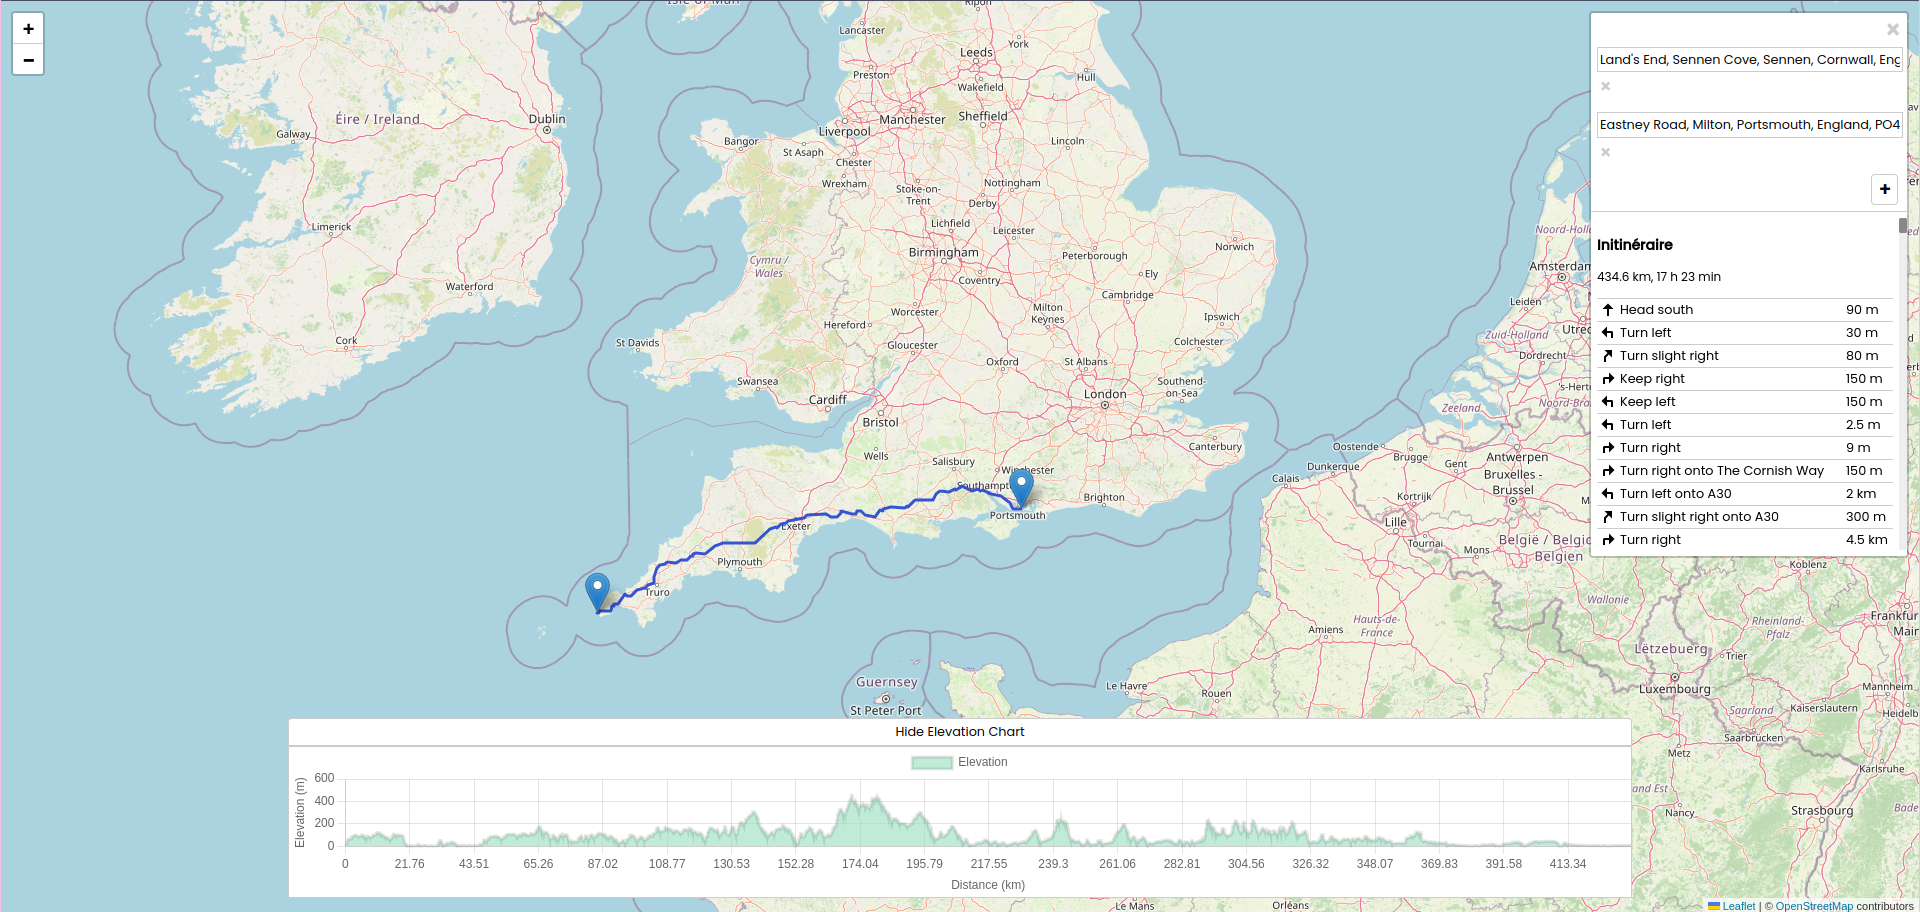
\includegraphics[width=425px]{figures/Progress Images/Iteration-1/SR28/Basic Elevation Plot Show Functionality.png}
    \caption{Basic Elevation Plot Show}
    % \label{fig:basic-elev-plot-show}
\end{figure}

\begin{figure}[!ht]
    \centering
    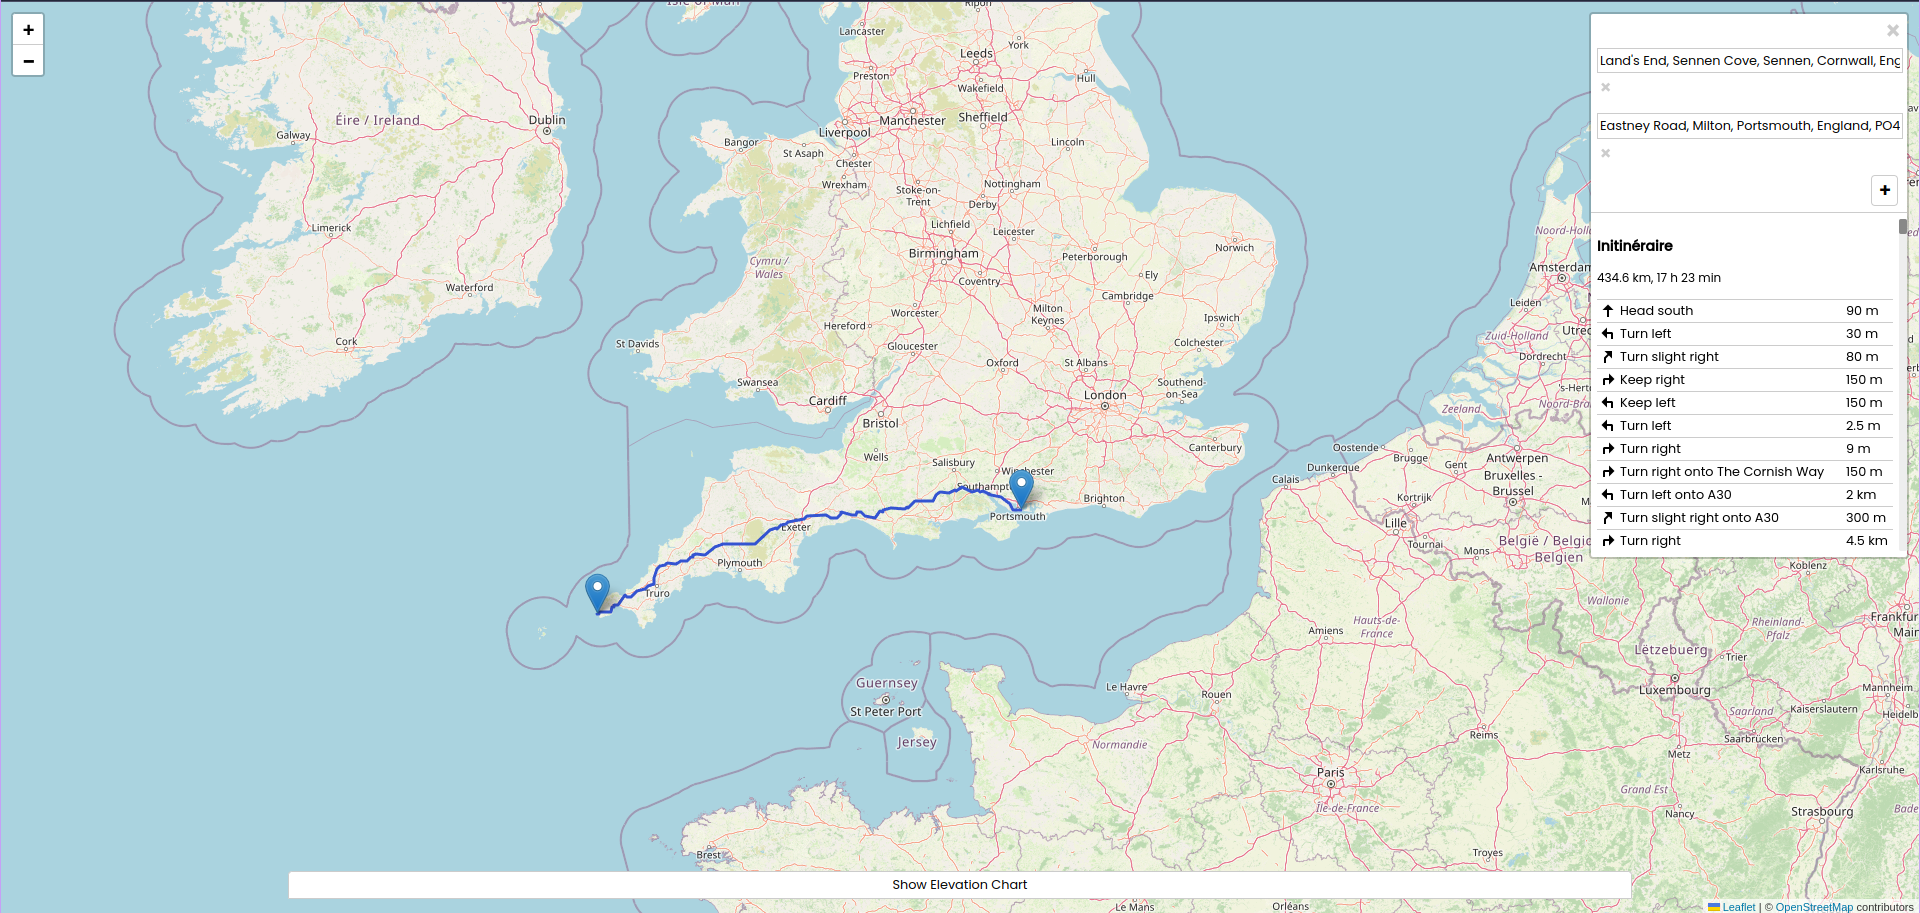
\includegraphics[width=425px]{figures/Progress Images/Iteration-1/SR28/Basic Elevation Plot Hide Functionality.png}
    \caption{Basic Elevation Plot Hide}
    % \label{fig:basic-elev-plot-hide}
\end{figure}


% \chapter{Increment 3 Screenshots}

\begin{figure}[!ht]
    \centering
    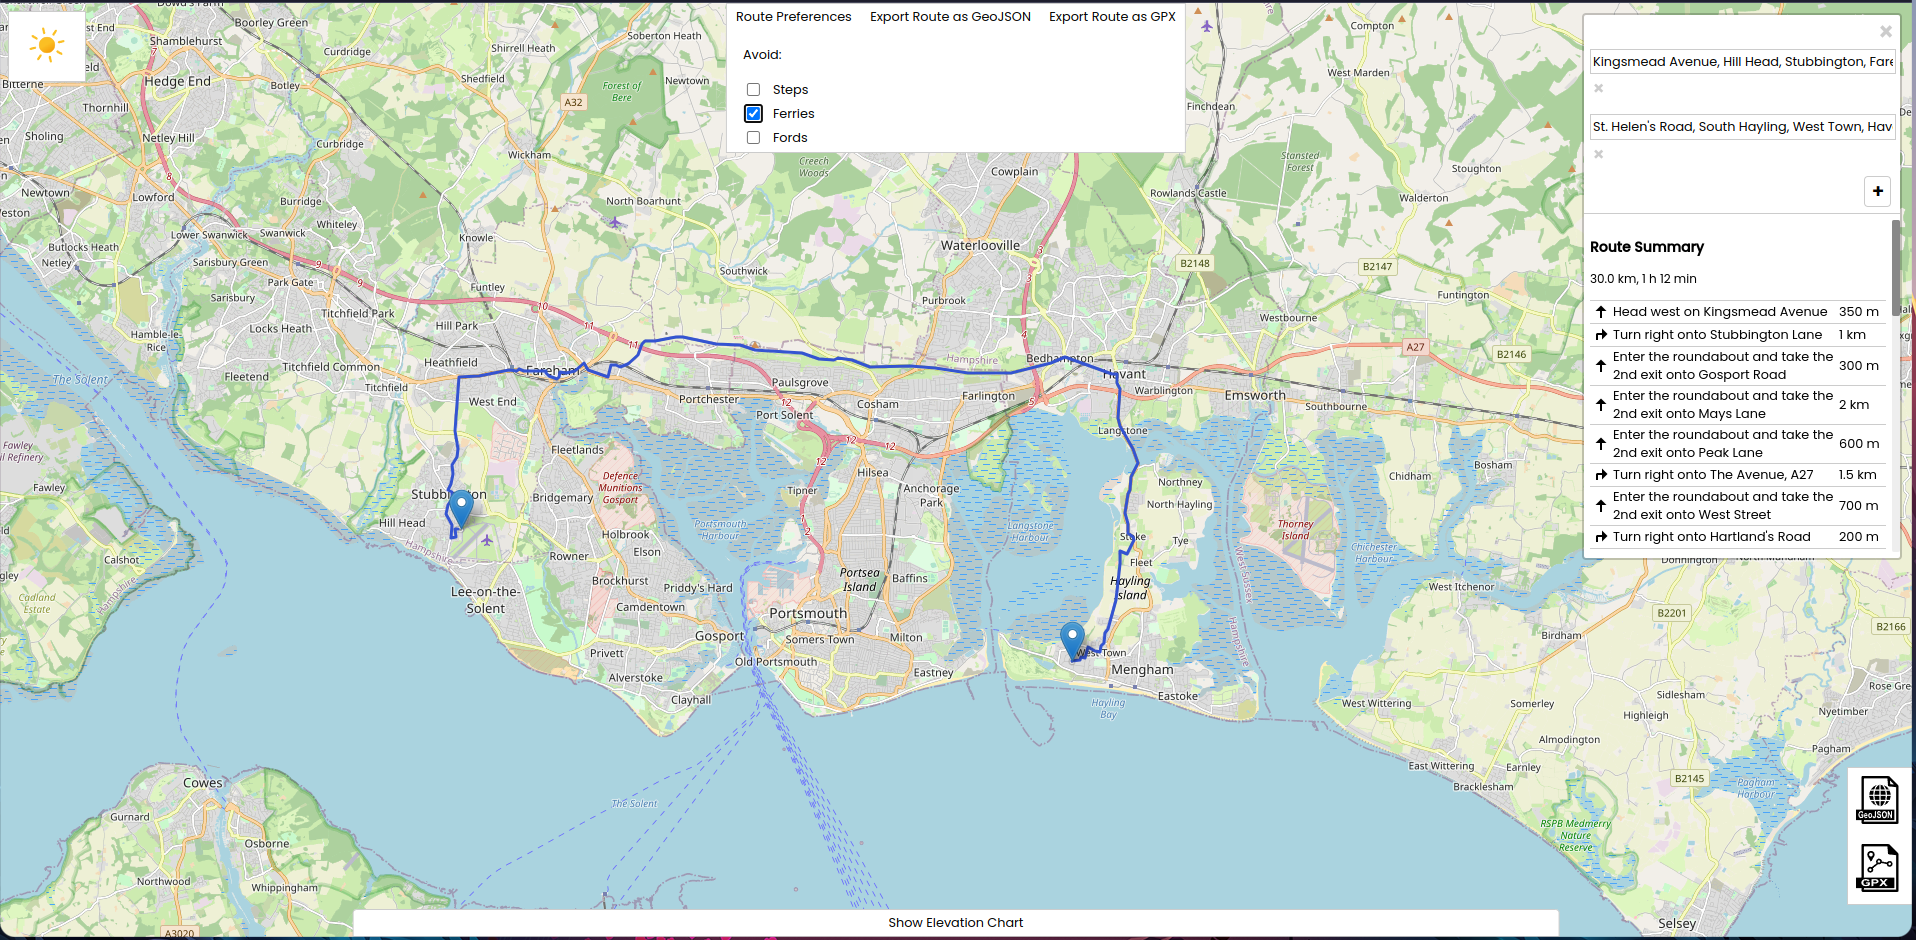
\includegraphics[width=425px]{figures/Progress Images/Iteration-1/SR7/SR9 Top Panel added and Avoid functionality implemented Avoid Ferries Example.png}
    \caption{Top Panel Added}
    % \label{fig:Top-Panel-added}
\end{figure}

\begin{figure}[!ht]
    \centering
    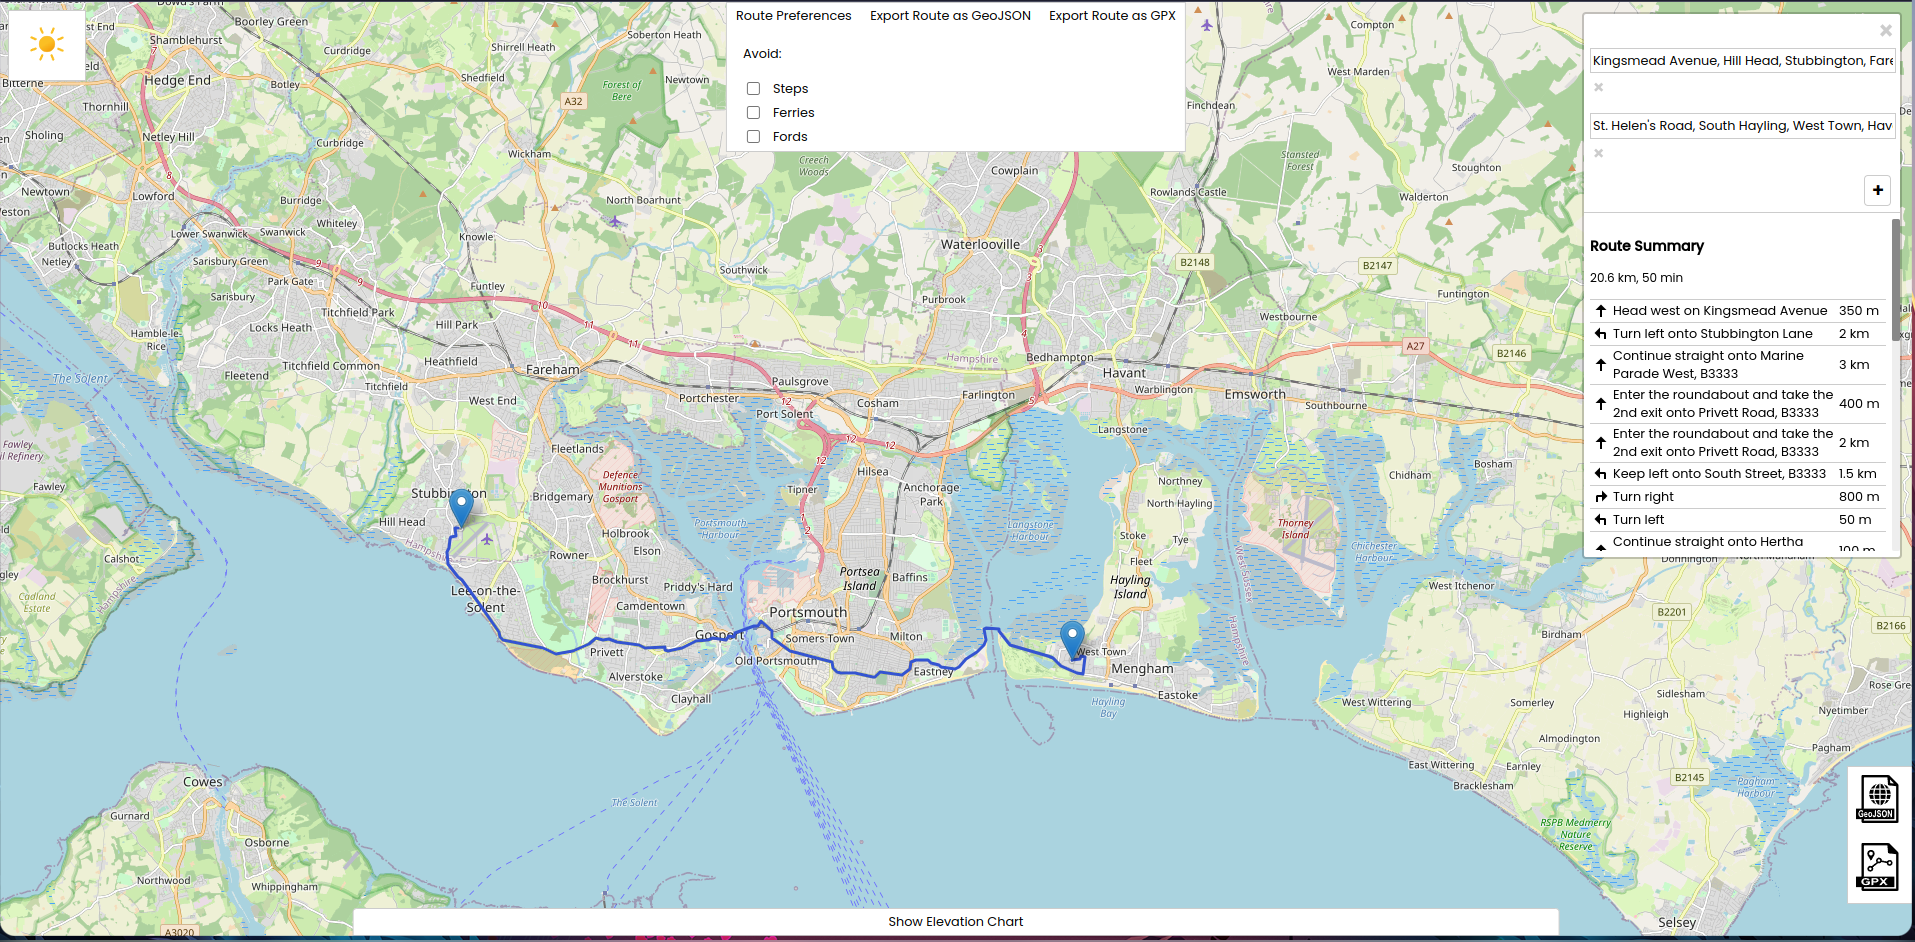
\includegraphics[width=425px]{figures/Progress Images/Iteration-1/SR7/SR9 Top Panel added and Avoid functionality implemented.png}
    \caption{Top Panel Added 2}
    % \label{fig:Top-Panel-added2}
\end{figure}

\begin{figure}[!ht]
    \centering
    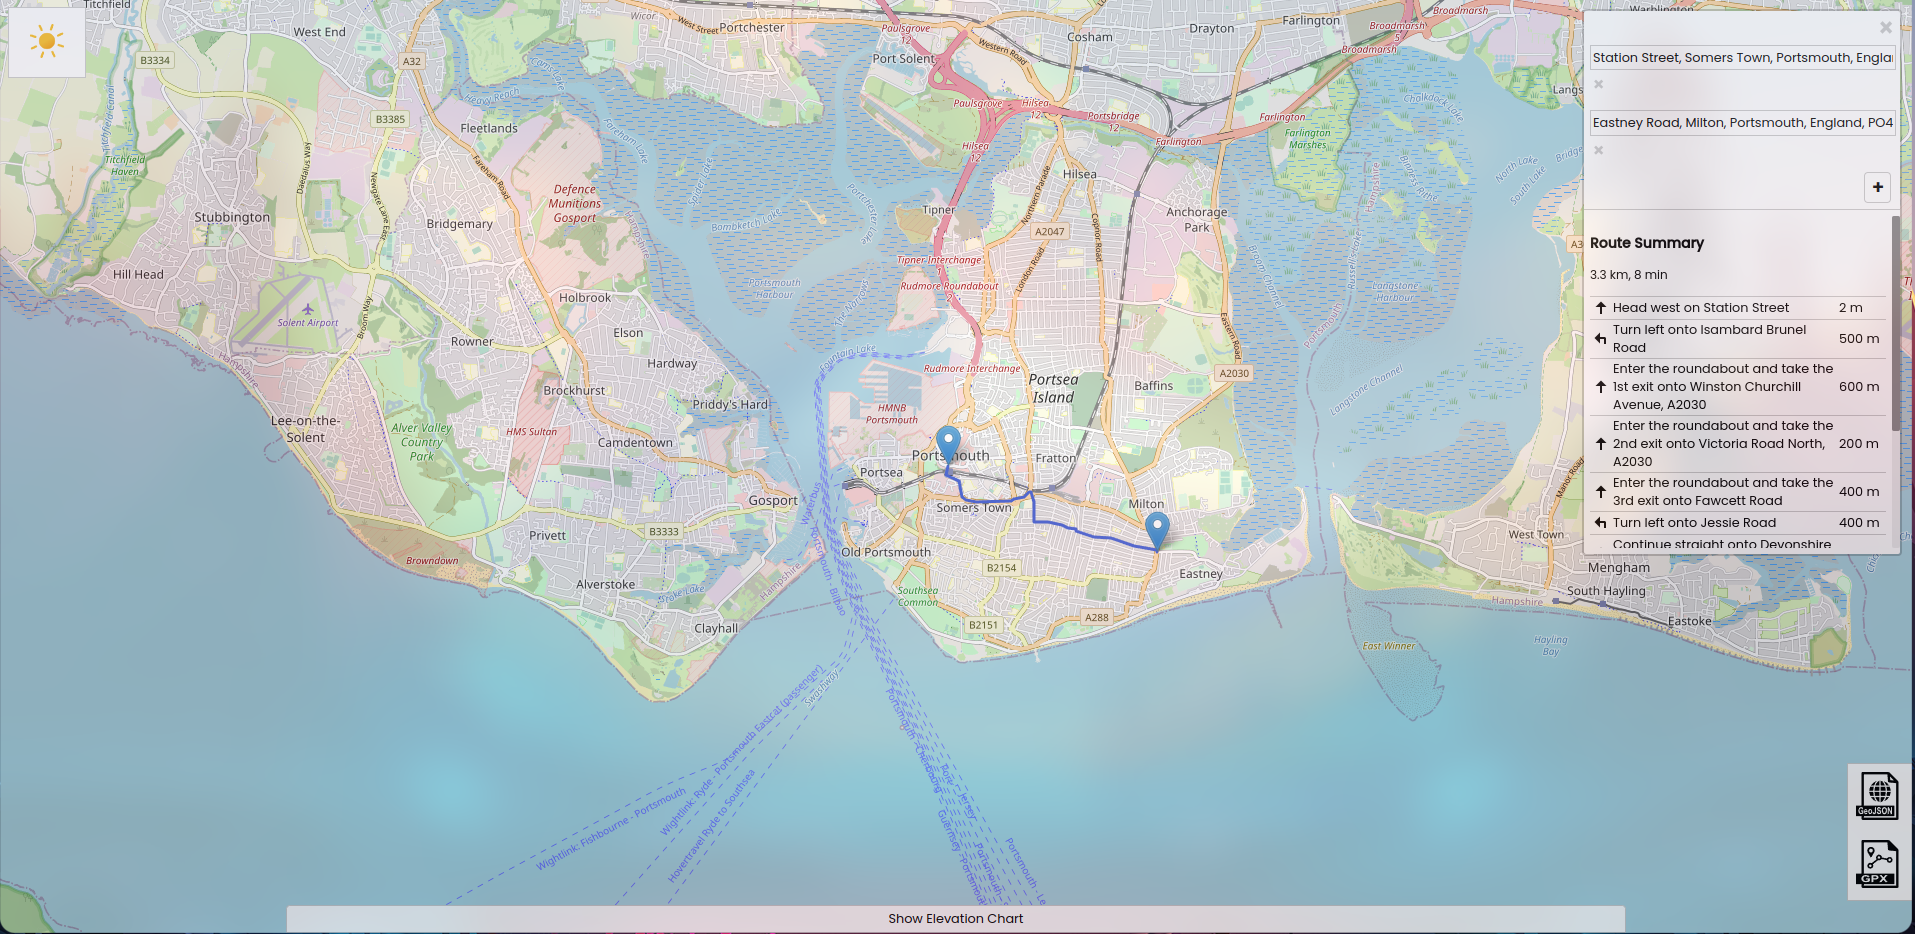
\includegraphics[width=425px]{figures/Progress Images/Iteration-1/SR12/SR13 GPX Icon Added (bottom right).png}
    \caption{GPX Icon Added}
    % \label{fig:gpx-icon-added}
\end{figure}

\begin{figure}[!ht]
    \centering
    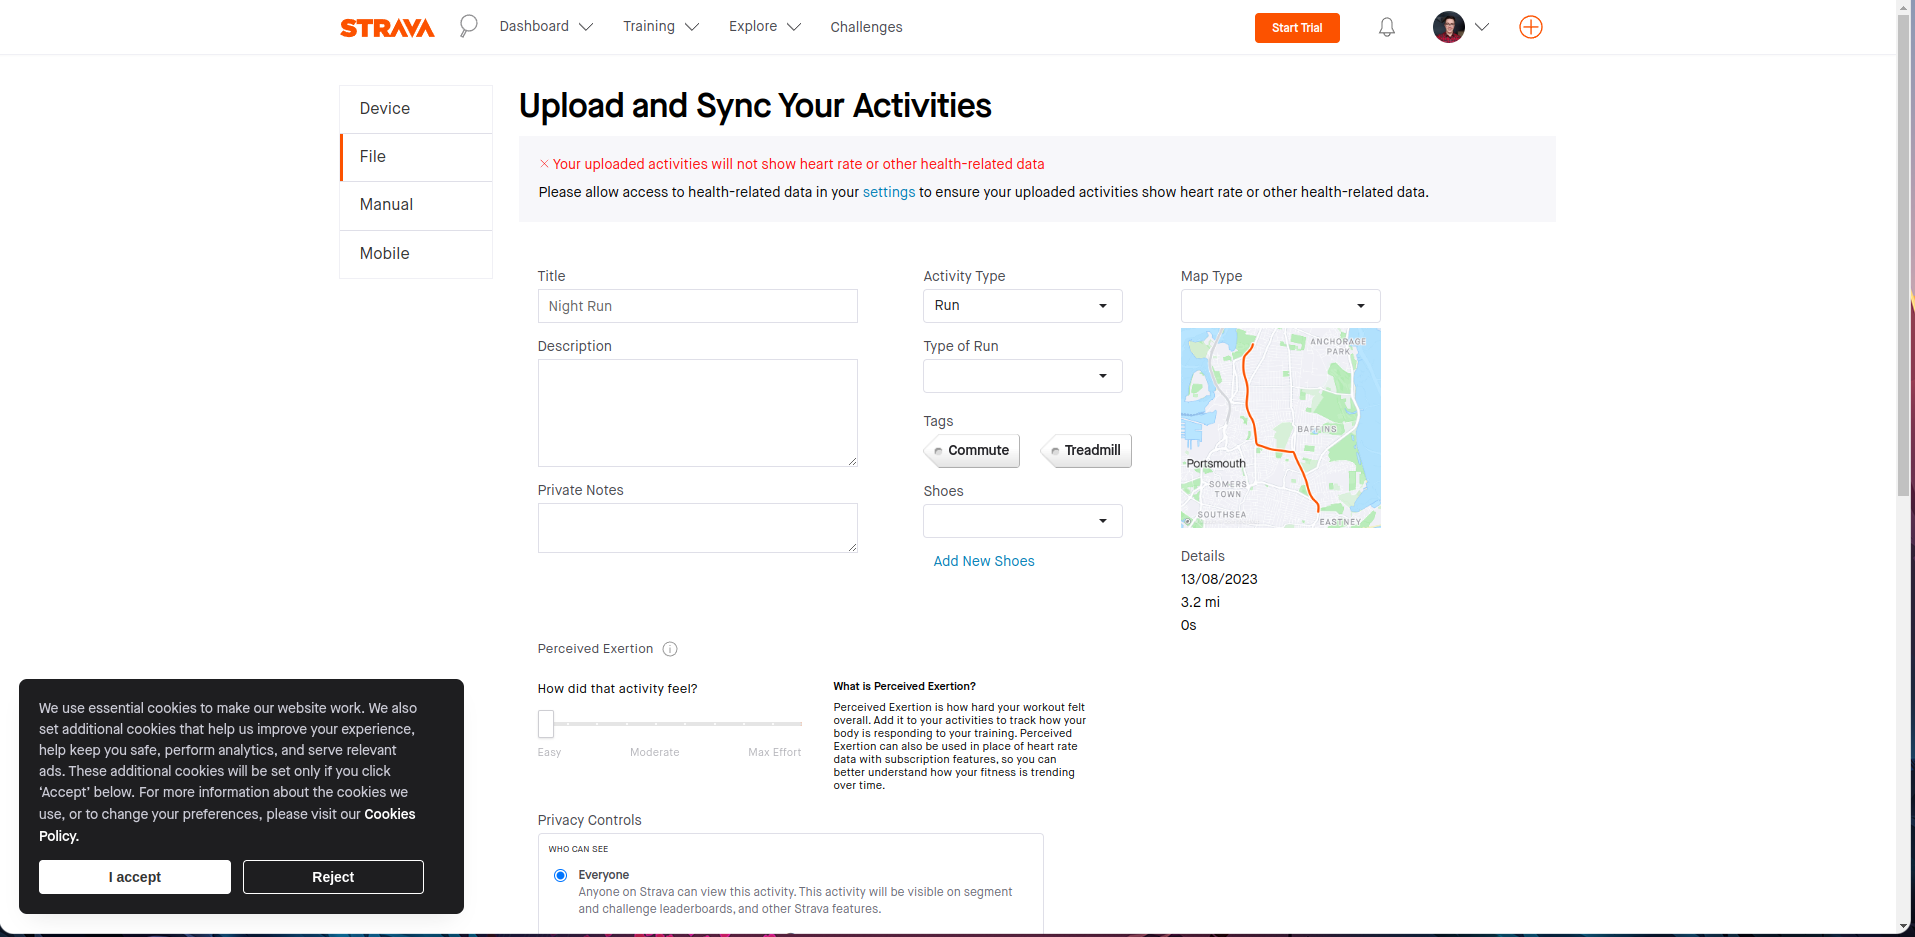
\includegraphics[width=425px]{figures/Progress Images/Iteration-1/SR12/SR13 GPX Successful upload Strava (manual).png}
    \caption{Manual Strava GPX Upload Test}
    % \label{fig:manual-strava-gpx}
\end{figure}

\begin{figure}[!ht]
    \centering
    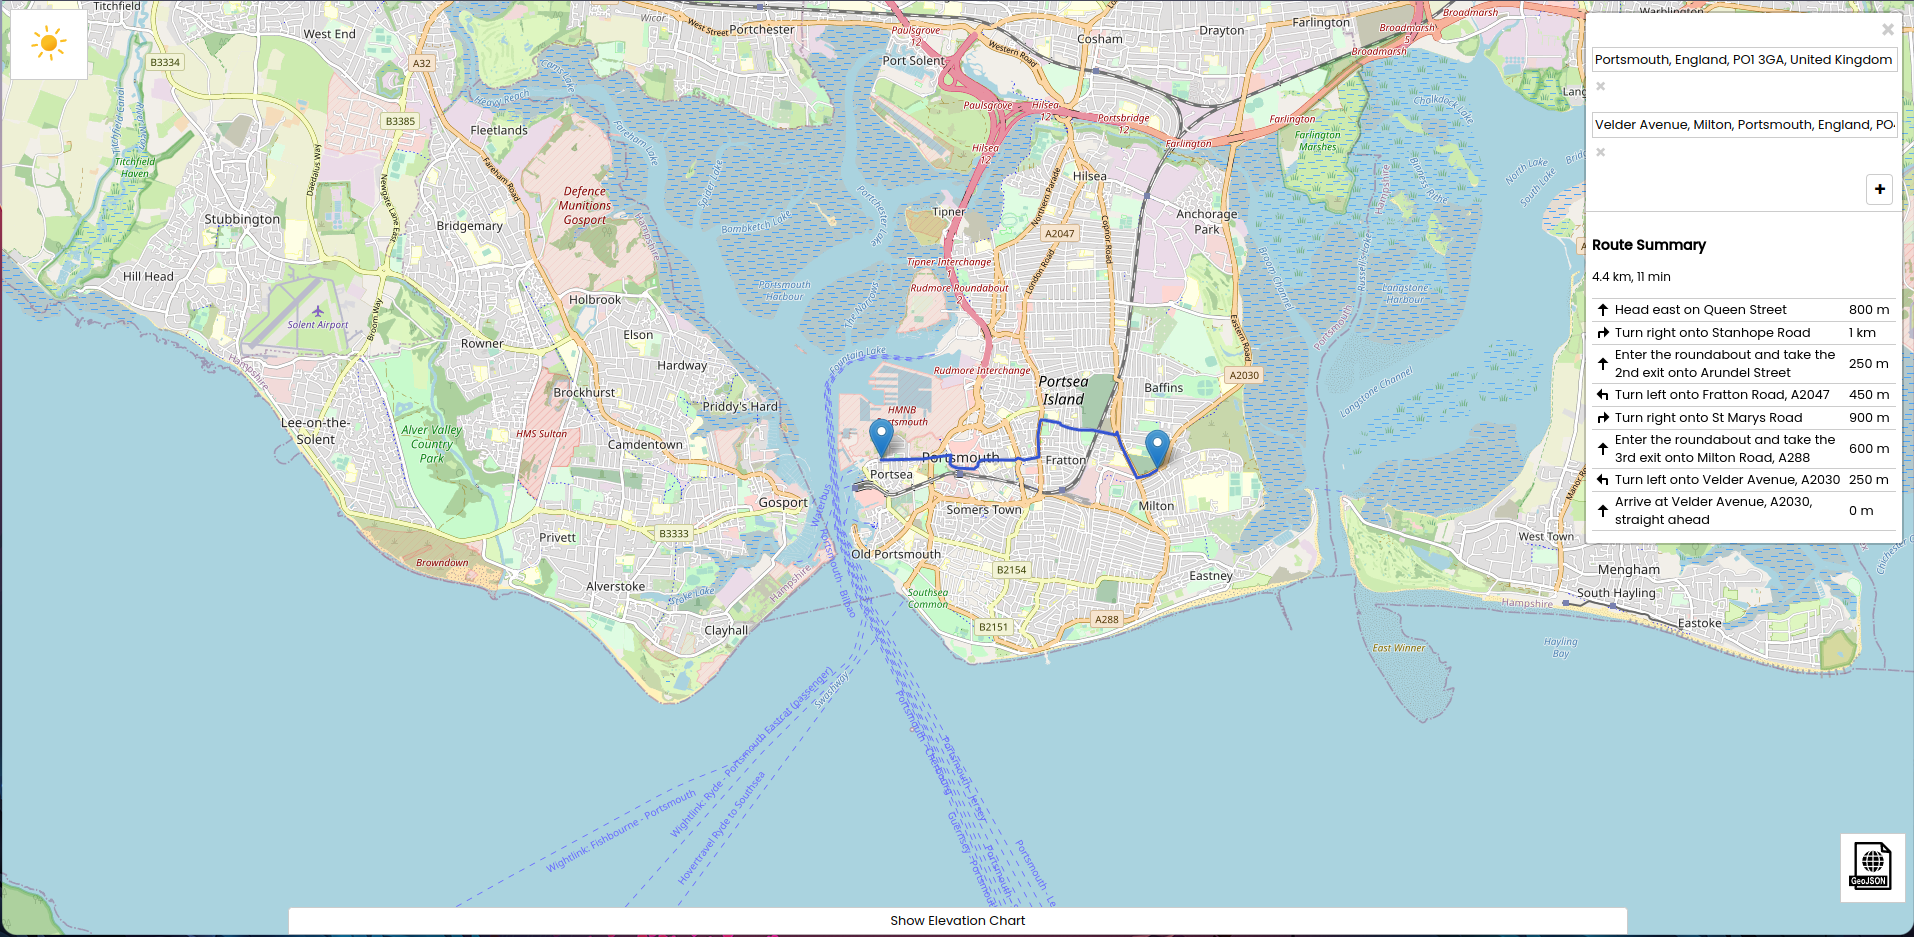
\includegraphics[width=425px]{figures/Progress Images/Iteration-1/SR12/SR14 GeoJSON Export.png}
    \caption{GeoJSON Export}
    % \label{fig:geojson-export}
\end{figure}

\begin{figure}[!ht]
    \centering
    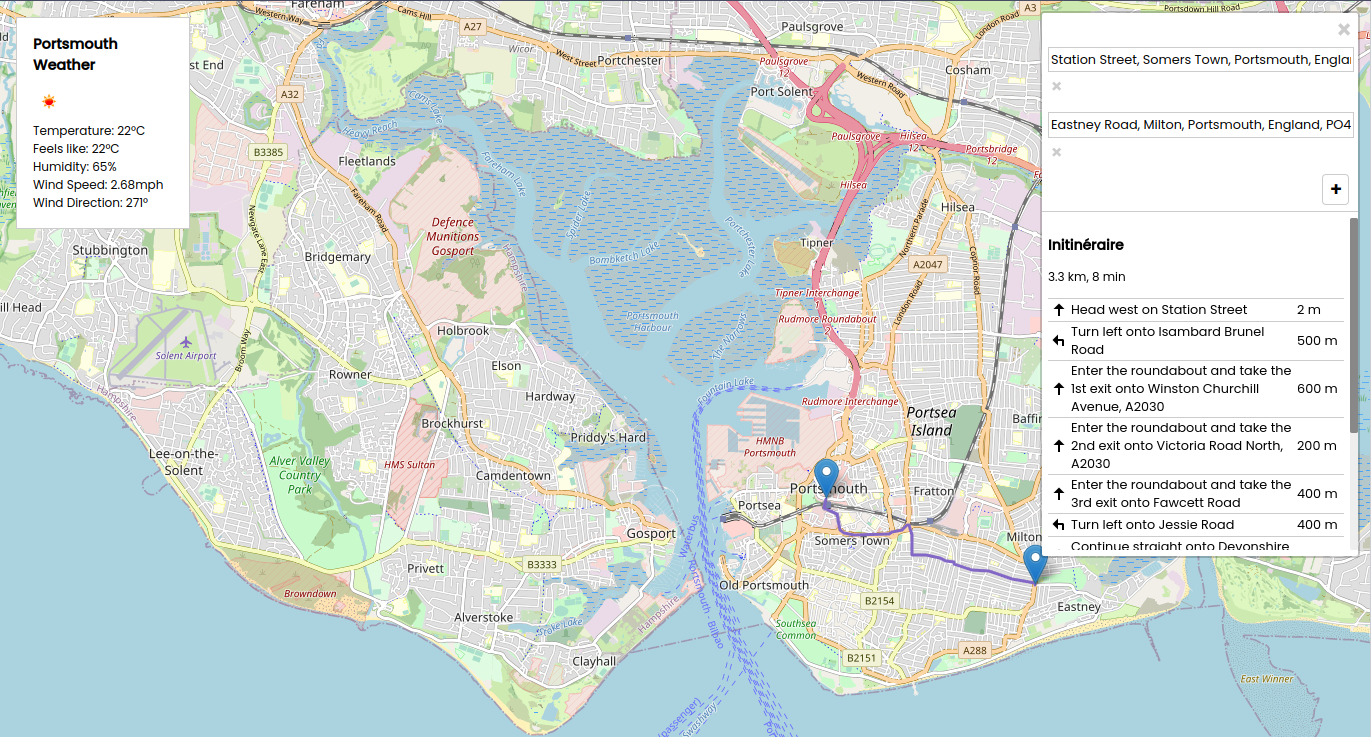
\includegraphics[width=425px]{figures/Progress Images/Iteration-1/SR19/Basic Weather Panel.png}
    \caption{Old Weather Panel}
    % \label{fig:basic-weather-panel2}
\end{figure}

\begin{figure}[!ht]
    \centering
    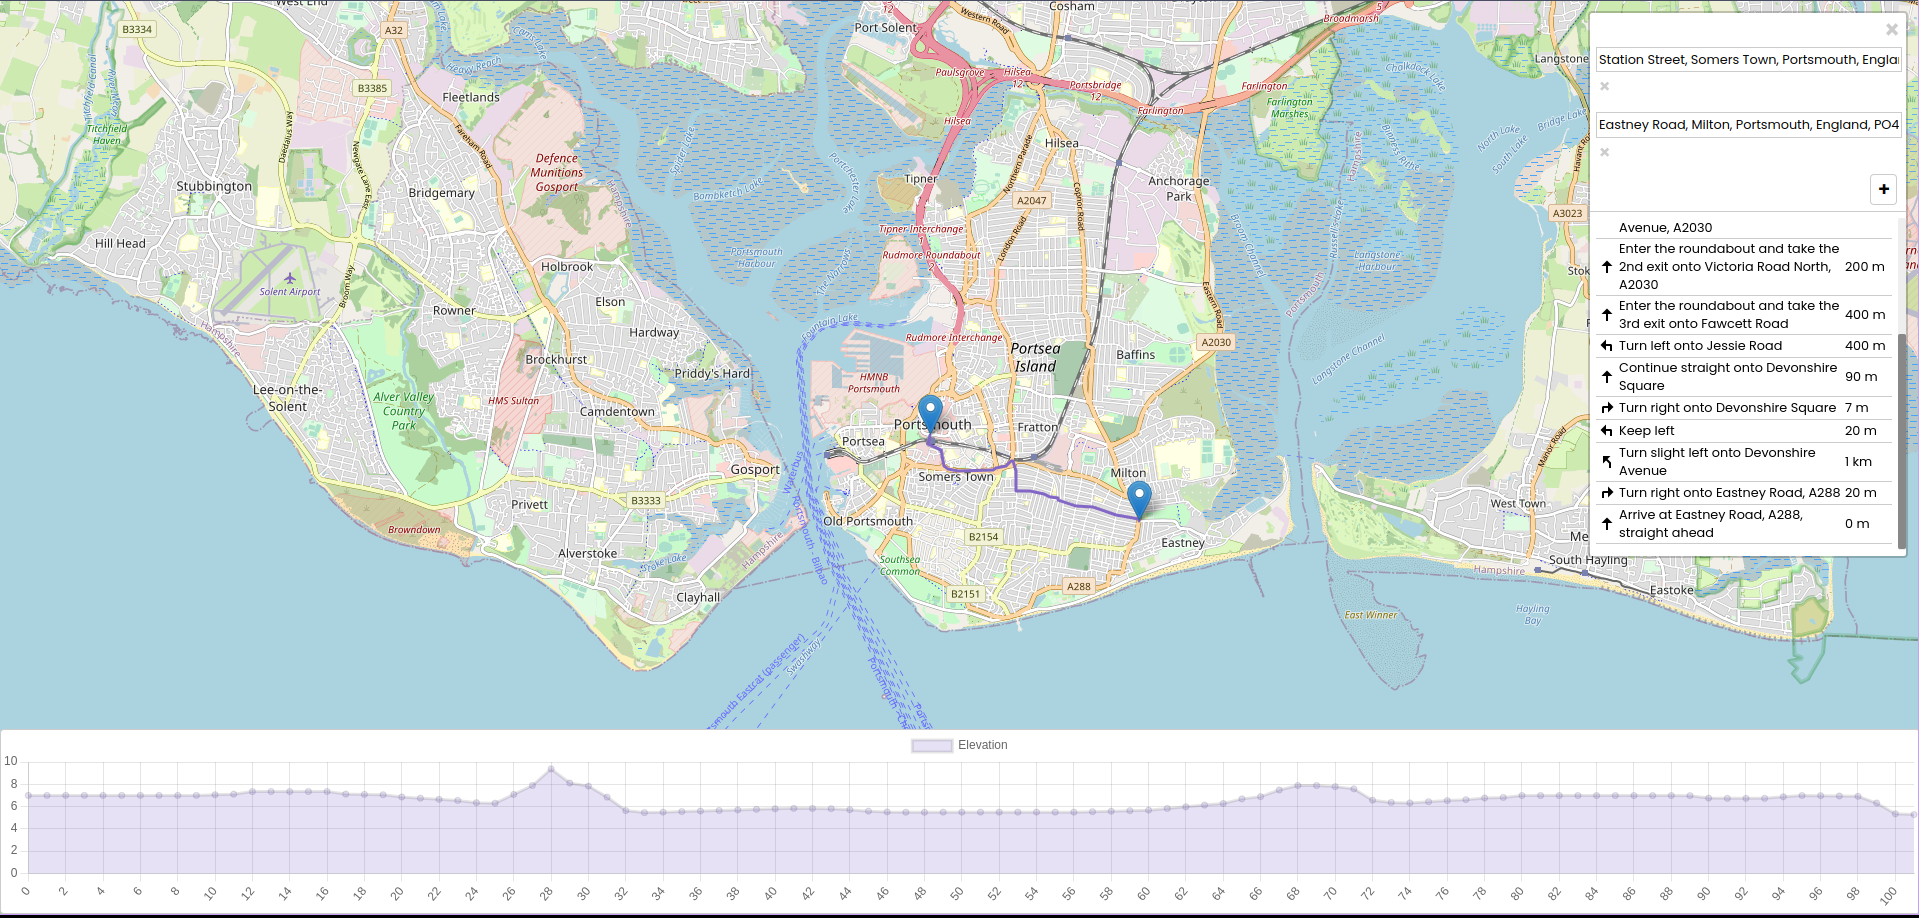
\includegraphics[width=425px]{figures/Progress Images/Iteration-1/SR28/Basic Elevation Plot.png}
    \caption{Basic Elevation Plot}
    % \label{fig:basic-elev-plot}
\end{figure}

\begin{figure}[!ht]
    \centering
    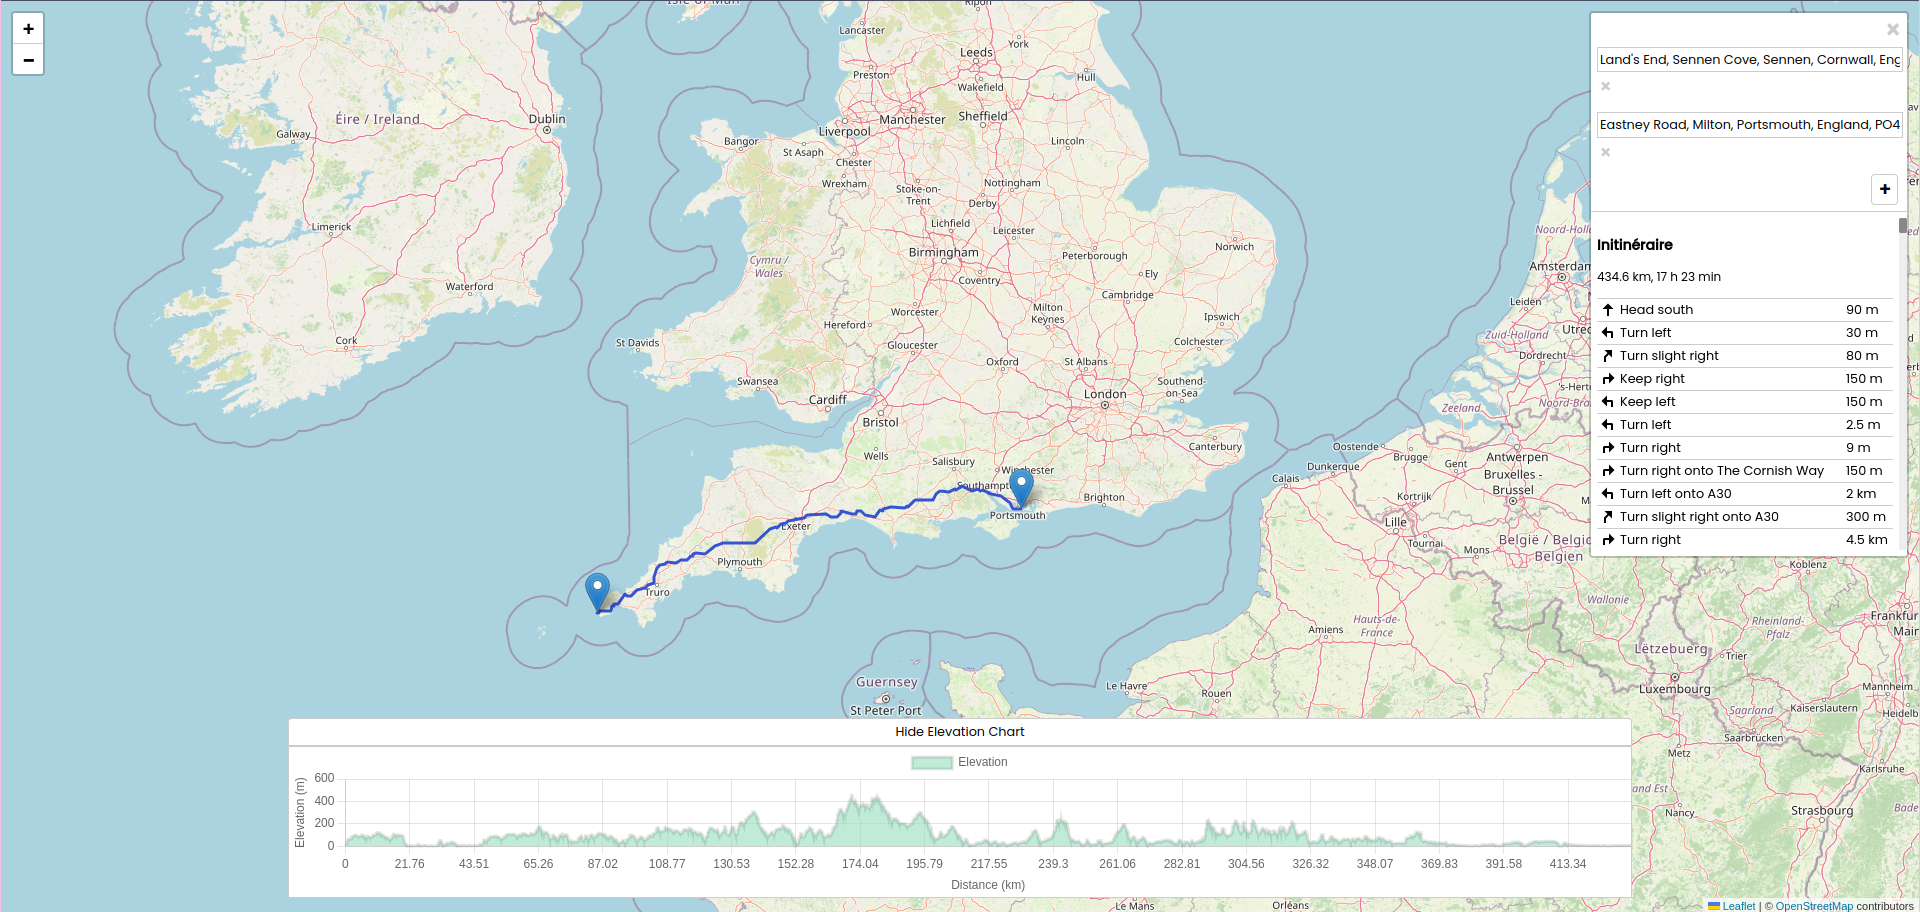
\includegraphics[width=425px]{figures/Progress Images/Iteration-1/SR28/Basic Elevation Plot Show Functionality.png}
    \caption{Basic Elevation Plot Show}
    % \label{fig:basic-elev-plot-show}
\end{figure}

\begin{figure}[!ht]
    \centering
    \includegraphics[width=425px]{figures/Progress Images/Iteration-1/SR28/Basic Elevation Plot Hide Functionality.png}
    \caption{Basic Elevation Plot Hide}
    % \label{fig:basic-elev-plot-hide}
\end{figure}


% \chapter{Project Meetings}
\begin{figure}[ht!]
    \centering
    \includegraphics[width=300px]{figures/project-meeting-1.png}
    \caption{Project Meeting Example 1}
    \label{fig:meeting-1}
\end{figure}

\begin{figure}[ht!]
    \centering
    \includegraphics[width=300px]{figures/project-meeting-2.png}
    \caption{Project Meeting Example 2}
    \label{fig:meeting-2}
\end{figure}

\begin{figure}[ht!]
    \centering
    \includegraphics[width=300px]{figures/project-meeting-3.png}
    \caption{Project Meeting Example 3}
    \label{fig:meeting-3}
\end{figure}

\begin{figure}[ht!]
    \centering
    \includegraphics[width=300px]{figures/project-meeting-4.png}
    \caption{Project Meeting Example 4}
    \label{fig:meeting-4}
\end{figure}

\label{pm:supervisor_meeting_list}
\begin{itemize}
    \item \textbf{Meeting 1 - 26th September 2023}
    \begin{itemize}
        \item Discussion of the initial project idea.
        \item Discussion of different approaches to the project.
        \item Discussion of the best way to work with the supervisor.
    \end{itemize}
    \item \textbf{Meeting 2 - 5th October 2023}
    \begin{itemize}
        \item Feedback on initial draft project initiation document.
        \item Outlining overall project objectives.
    \end{itemize}
    \item \textbf{Meeting 3 - 11th October 2023}
    \begin{itemize}
        \item Finalise and submit project initiation document.
        \item Discussion of ethics application.
        \item Discussion of potential primary research methods.
    \end{itemize}
    \item \textbf{Meeting 4 - 18th October 2023}
    \begin{itemize}
        \item Demo and feedback of initial research prototype application.
        \item Demo and feedback of initial basic artefact setup.
        \item Discussion of potential future features.
    \end{itemize}
    \item \textbf{Meeting 5 - 25th October 2023}
    \begin{itemize}
        \item Feedback on document progress so far, working towards literature review.
        \item Discussion on ways to rank and compare feedback from the research application.
    \end{itemize}
    \item \textbf{Meeting 6 - 30th October 2023}
    \begin{itemize}
        \item Feedback on literature review.
        \item Discussion of requirements using research feedback.
    \end{itemize}
    \item \textbf{Meeting 7 - 14th November 2023}
    \begin{itemize}
        \item Feedback on complete literature review.
        \item Feedback and discussion of requirements.
        \item Further discussion of potential future features on top of requirements.
    \end{itemize}
    \item \textbf{Meeting 8 - 29th November 2023}
    \begin{itemize}
        \item Requirements mostly finalised, feedback received.
        \item Discussion on the design of the artefact.
    \end{itemize}
    \item \textbf{Meeting 9 - 8th December 2023}
    \begin{itemize}
        \item Final feedback on project so far for 2023.
        \item Discussion of development/sprint plan for January 2024.
        \item Discussion of plan post-development.
    \end{itemize}
    \item \textbf{Meeting 10 - 10th January 2024}
    \begin{itemize}
        \item Feedback on development progress so far.
        \item Agreement made to delay meetings for 3-4 weeks to allow for development.
        \item Agreement on the plan for post-development (3-4 weeks).
    \end{itemize}
    \item \textbf{Meeting 11 - 9th February 2024}
    \begin{itemize}
        \item Feedback on development
        \item Discussion of end-goal, final artefact/document.
        \item Discussion of the plan for the project stages.
    \end{itemize}
    \item \textbf{Meeting 12 - 16th February 2024}
    \begin{itemize}
        \item Feedback on Design and Implementation chapters.
        \item Discussion of the use of unplanned extra time to improve artefact.
    \end{itemize}
    \item \textbf{Meeting 13 - 23rd February 2024}
    \begin{itemize}
        \item Guidance provided for improvements to report.
        \item Discussion on how to use extra time.
    \end{itemize}
    \item \textbf{Meeting 14 - 28th February 2024}
    \begin{itemize}
        \item Further guidance provided and feedback given on improvements made.
        \item Discussion to build a script to create a Gantt chart from the GitHub repository.
    \end{itemize}
    \item \textbf{Meeting 15 - 13th March 2024}
    \begin{itemize}
        \item Feedback on final report.
        \item Improvements suggested.
        \item Demo of Gantt/commit graph app.
    \end{itemize}
\end{itemize}

% \chapter{Project Initiation Document}
\includepdf[pages=-]{figures/PID.pdf}

\end{document}
